In this section, we study the discrimination of a boosted, hadronically decaying $W$ boson (signal) against a gluon-initiated jet
background, comparing the performance of various groomed jet
masses and substructure variables.
%, and BDT combinations of groomed mass
%and substructure observables. 
%We produce ROC
%curves that elucidate the performance of the various groomed mass and
%substructure variables.
A range of different distance parameters for the \antikt jet
algorithm are explored, in a range of different leading jet \pt bins.
%(lead jet \pt 300-400 GeV, 500-600 GeV, 1.0-1.1 TeV). 
This allows us to determine the
performance of observables as a function of jet radius and jet boost, and to see
where different approaches may break down. The groomed
mass and substructure variables are then combined in a BDT as described in Section~\ref{sec:multivariate}, and the performance of the resulting BDT discriminant
explored through ROC curves to understand the degree to which
variables are correlated, and how
this changes with jet boost and jet radius. 

\subsection{Methodology}

These studies use the $WW$ samples as signal and the dijet $gg$ as background, described previously in Section~\ref{sec:samples}. Whilst only gluonic backgrounds
are explored here, the conclusions regarding the dependence of the
performance and correlations on the jet boost and radius are not
expected to be substantially different for quark backgrounds; we will
see that the differences in the substructure properties of quark- and
gluon-initiated jets, explored in the last section, are significantly
smaller than the differences between $W$-initiated and gluon-initiated jets.

As in the $q/g$ tagging studies, the showered events were clustered with \textsc{FastJet}
3.03 using
the \antikt~algorithm with jet radii of $R = 0.4,\, 0.8,\, 1.2$. In
both signal and background samples, an upper and lower cut on
the leading jet $\pt$ is applied after showering/clustering, to ensure
similar $\pt$ spectra for signal and background in each \pt bin. The bins
in leading jet \pt that are considered are 300-400 \GeV, 500-600 \GeV,
1.0-1.1 \TeV, for the 300-400 \GeV, 500-600 \GeV,
1.0-1.1 \TeV parton \pt slices respectively. The jets then have various
grooming algorithms applied and substructure observables
reconstructed as described in
Section~\ref{sec:substructure}. The substructure observables
studied in this section are: 

\begin{itemize}
\item Ungroomed, trimmed (\mtrim), and pruned (\mprun) jet 
masses.
\item Mass output from the modified mass drop tagger (\mmdt).
\item Soft drop mass with $\beta=2$ (\msd). 
\item 2-point energy correlation function ratio $C_2^{\beta=1}$  (we also studied $\beta=2$ but do not show its results because it showed poor discrimination power).
\item $N$-subjettiness ratio $\tau_2 / \tau_1$ with $\beta=1$ ($\tau_{21}^{\beta=1}$) and with axes computed using one-pass $k_t$ axis optimization (we also studied $\beta=2$ but did not show its results because it showed poor discrimination power).
\item Pruned Qjet mass volatility, $\Gamma_{\rm Qjet}$.
\end{itemize}

% and have various
%jet grooming approaches applied as described in Section~\ref{sec:substructure}. The following event selection is then applied to these
%samples....(presumably this will vary depending on which kinematic bin
%is used, as will the actual samples used - maybe summarize in a table).
%
%Figure~\ref{fig:pt300_basics} shows a comparison of the
%leading jet \pT for the signal and background in the \pT 300-400 GeV bin, for the two different \antikt jet
%algorithm distance parameters explored in this bin (R=0.8 and R=1.2). Figures~\ref{fig:pt500_basics} and~\ref{fig:pt1000_basics}  show the same for the
%\pT = 500-600 GeV bin and \pT = 1.0-1.1 TeV bin respectively, where for
%the \pT = 1.0-1.1 TeV bin the distance parameter R=0.4 is also explored because the W radiation at this boost is typically confined to 
%a cone of this size.
%
%
%
%\begin{figure*}
%\centering
%\subfigure[\antikt R=0.8]{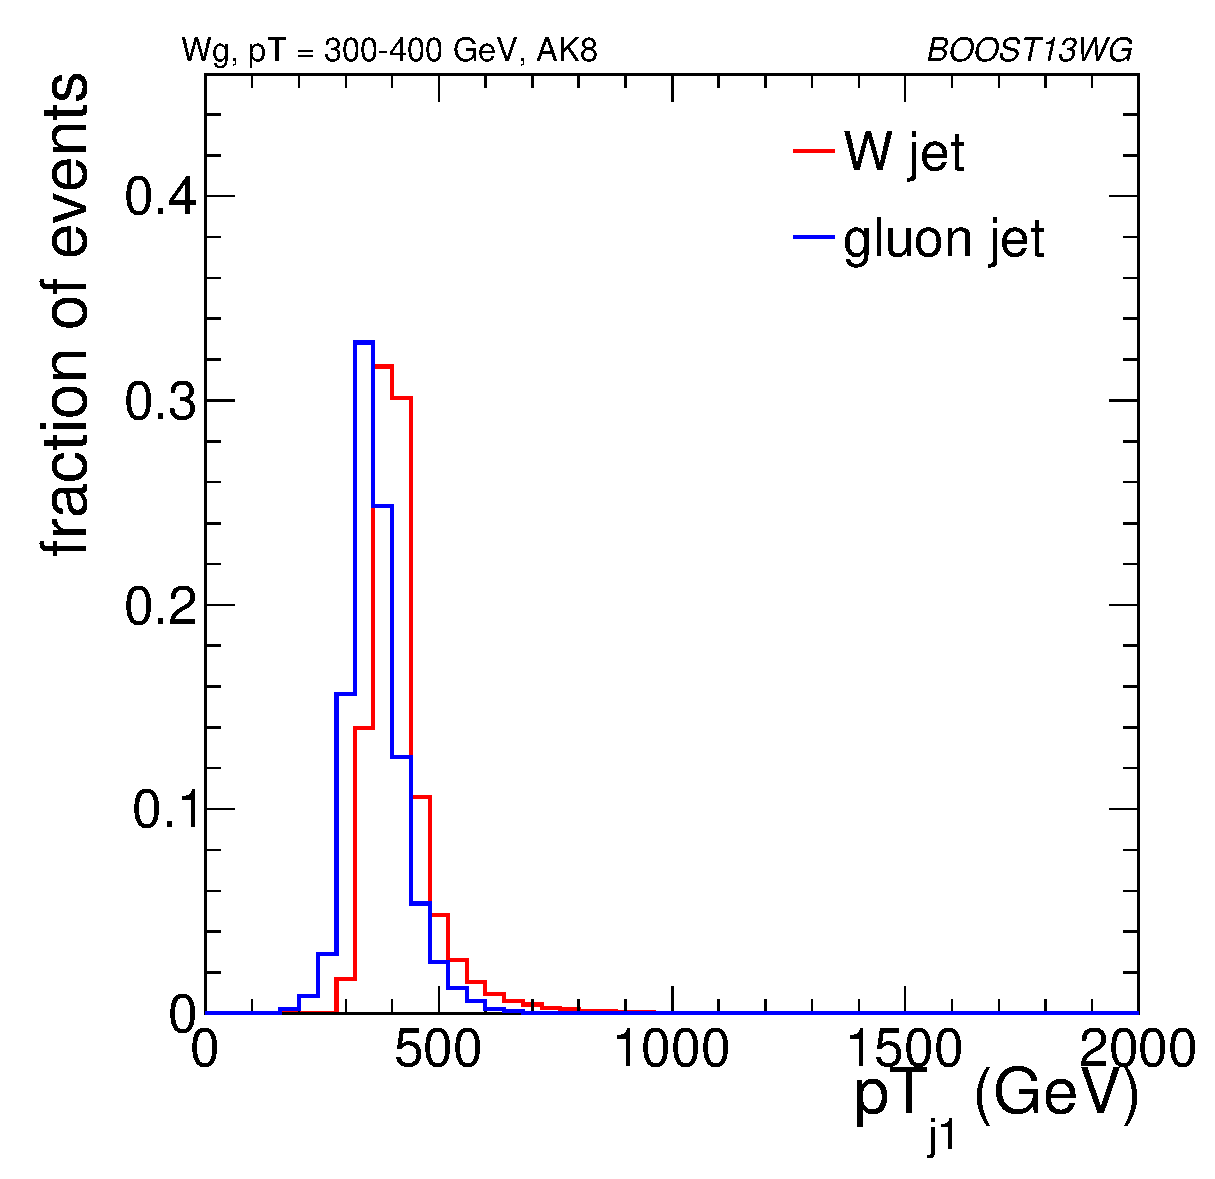
\includegraphics[width=0.30\textwidth]{./Figures/WTagging/pT300/AKtR08/jpt1.eps}}
%\subfigure[\antikt R=1.2]{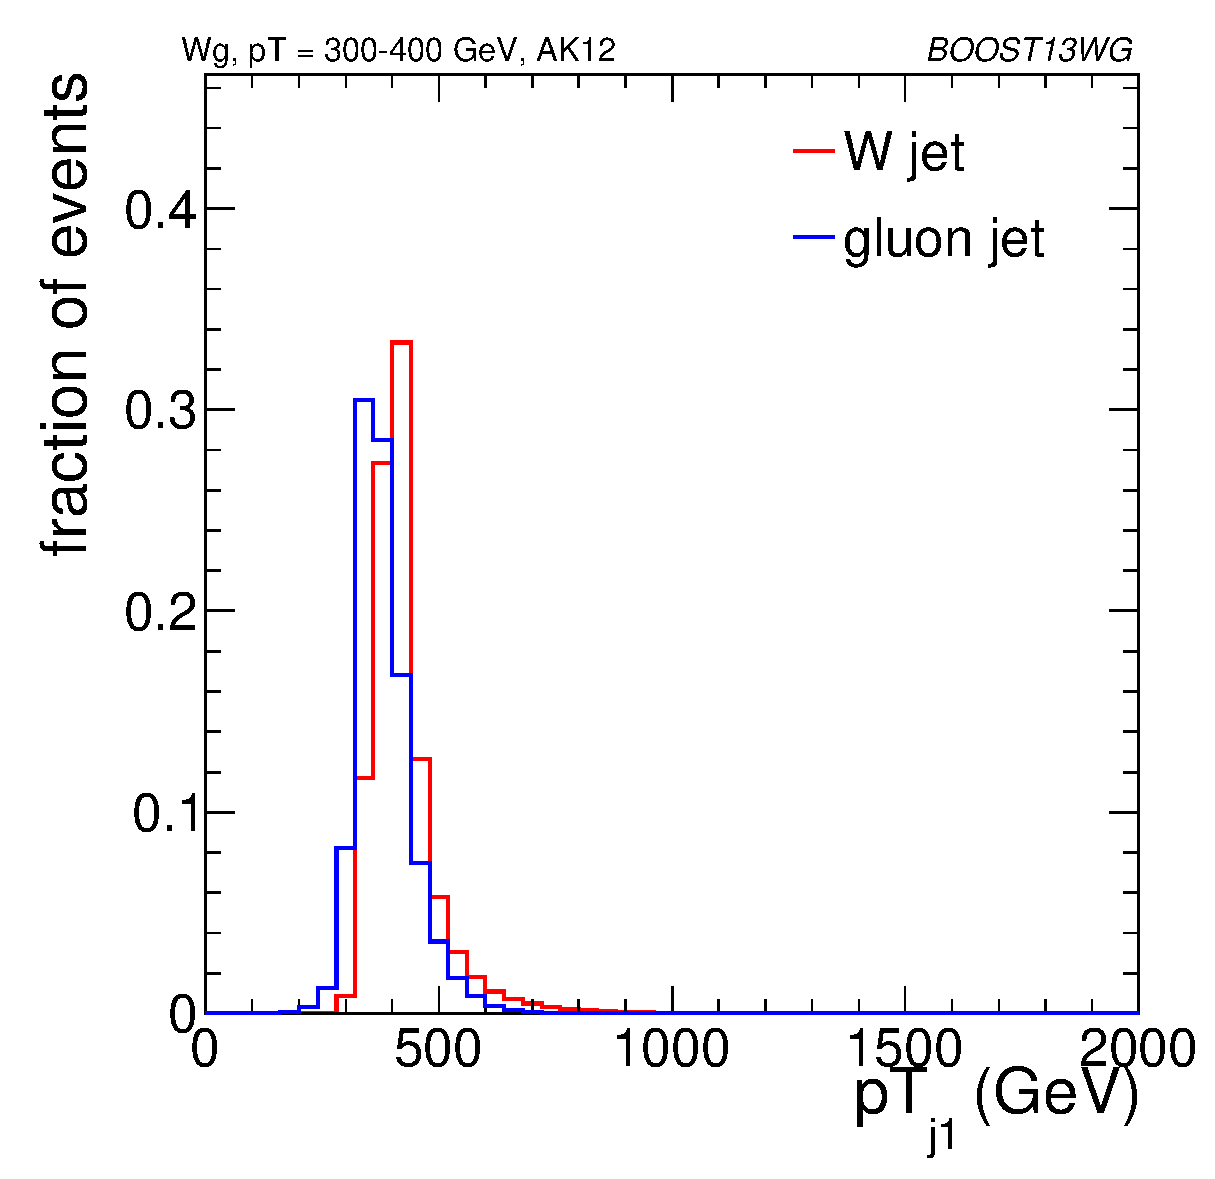
\includegraphics[width=0.30\textwidth]{./Figures/WTagging/pT300/AKtR12/jpt1.eps}}
%\caption{Comparisons of the leading jet \pT spectrum of the $gg$
%  background to the WW signal in the \pT 300-400 GeV bin using the
%  different \antikt jet distance parameters explored.}
%\label{fig:pt300_basics}
%\end{figure*}
%
%\begin{figure*}
%\centering
%\subfigure[\antikt R=0.8]{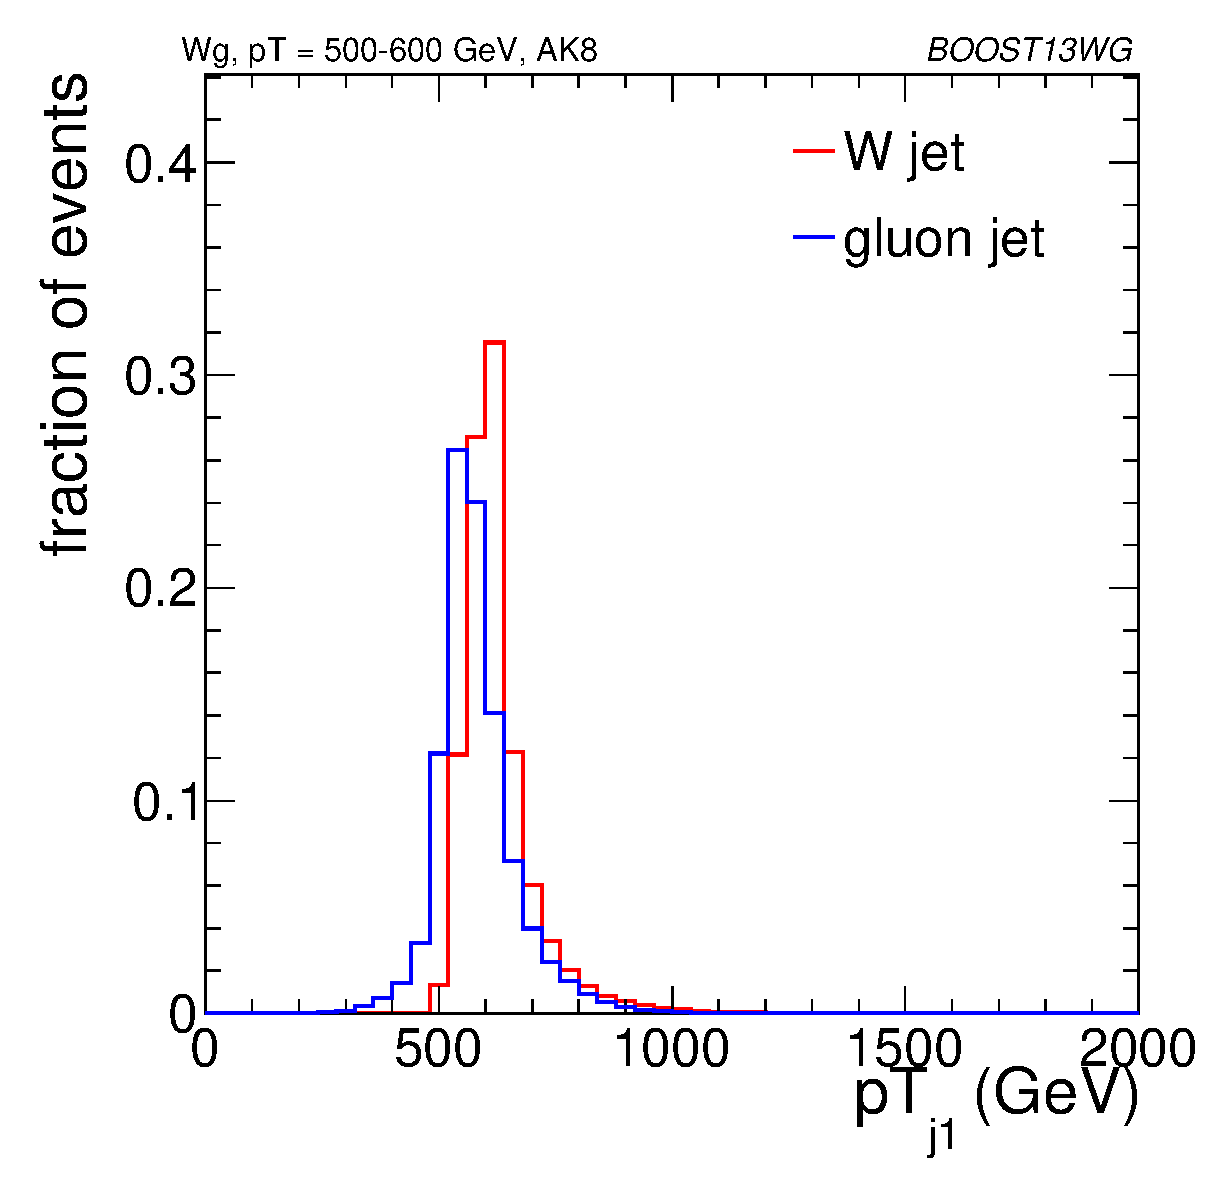
\includegraphics[width=0.30\textwidth]{./Figures/WTagging/pT500/AKtR08/jpt1.eps}}
%\subfigure[\antikt R=1.2]{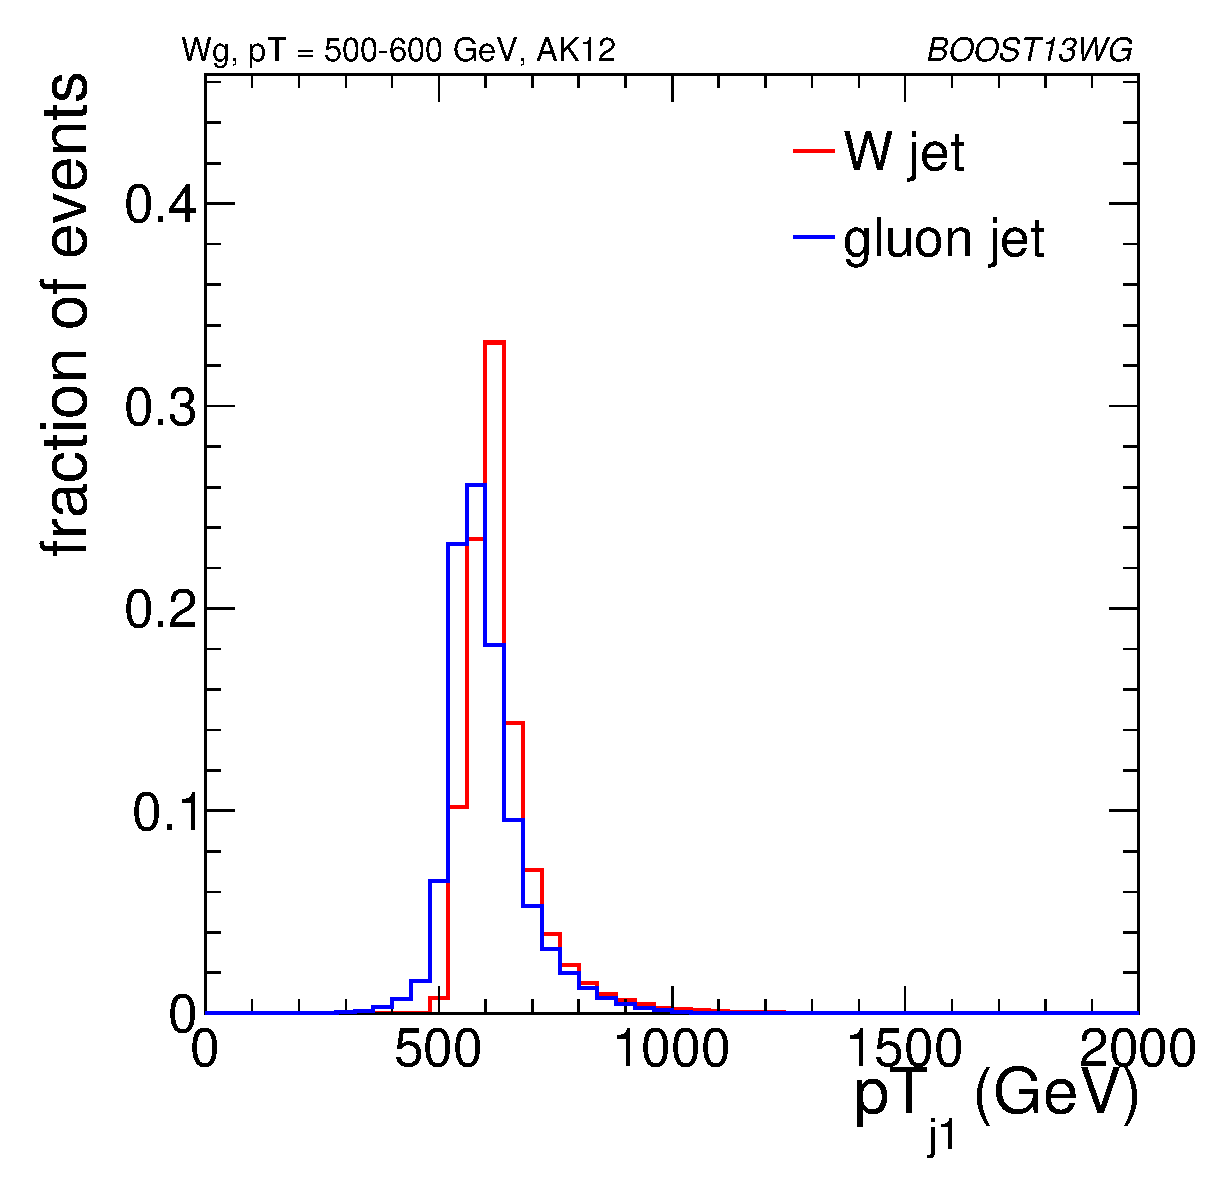
\includegraphics[width=0.30\textwidth]{./Figures/WTagging/pT500/AKtR12/jpt1.eps}}
%\caption{Comparisons of the leading jet \pT spectrum of the $gg$
%  background to the WW signal in the \pT = 500-600 GeV bin using the
%  different \antikt jet distance parameters explored.}
%\label{fig:pt500_basics}
%\end{figure*}
%
%\begin{figure*}
%\centering
%\subfigure[\antikt R=0.4]{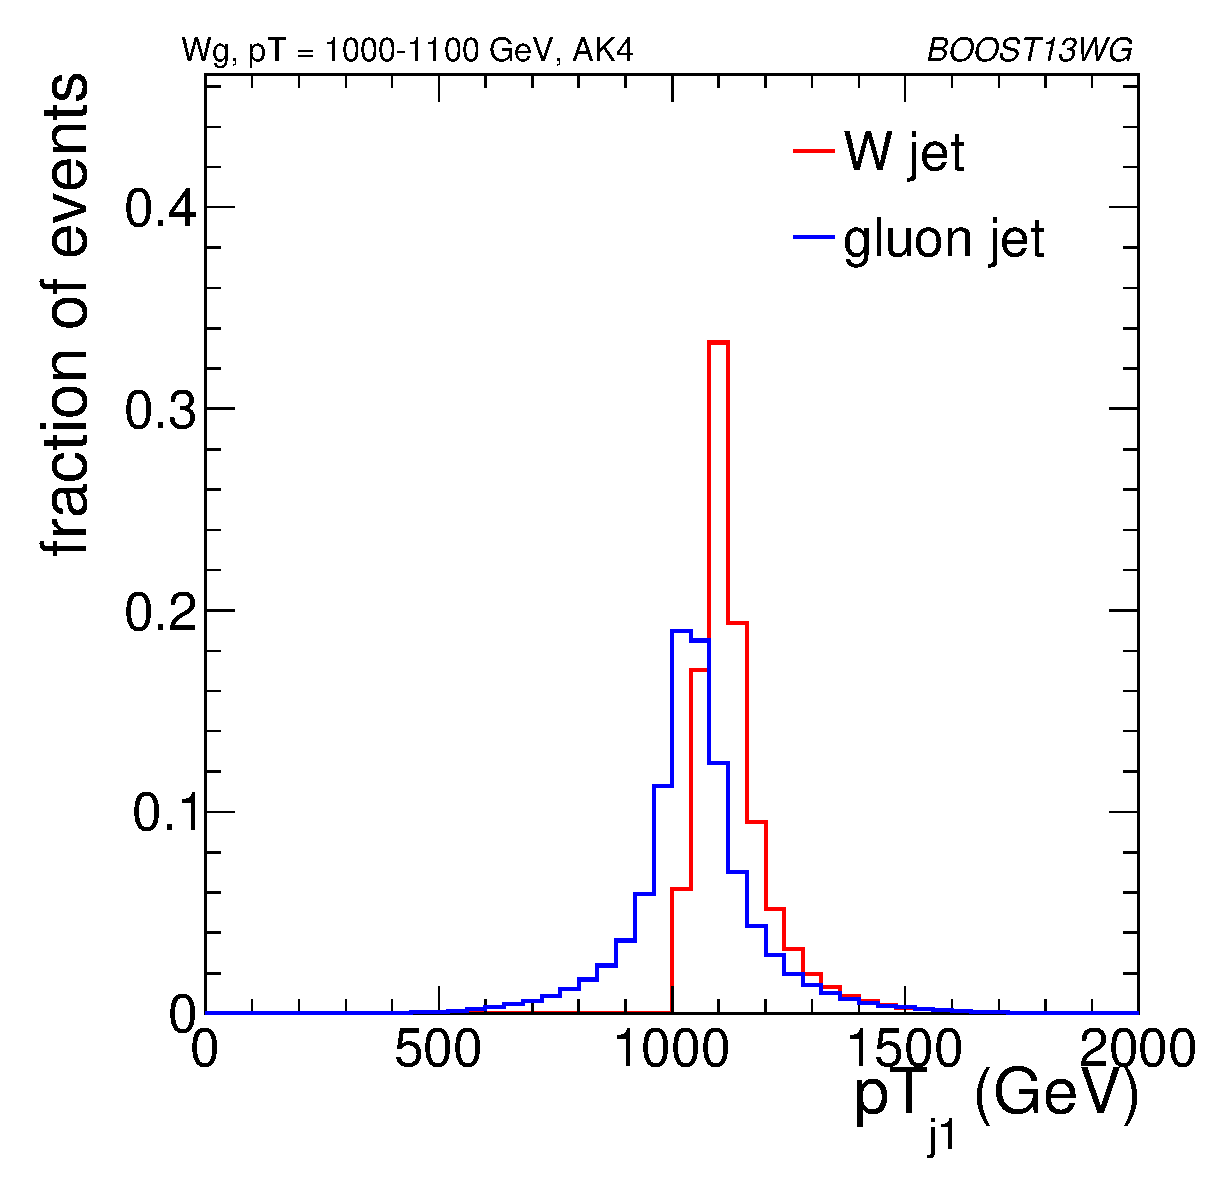
\includegraphics[width=0.30\textwidth]{./Figures/WTagging/pT1000/AKtR04/jpt1.eps}}
%\subfigure[\antikt R=0.8]{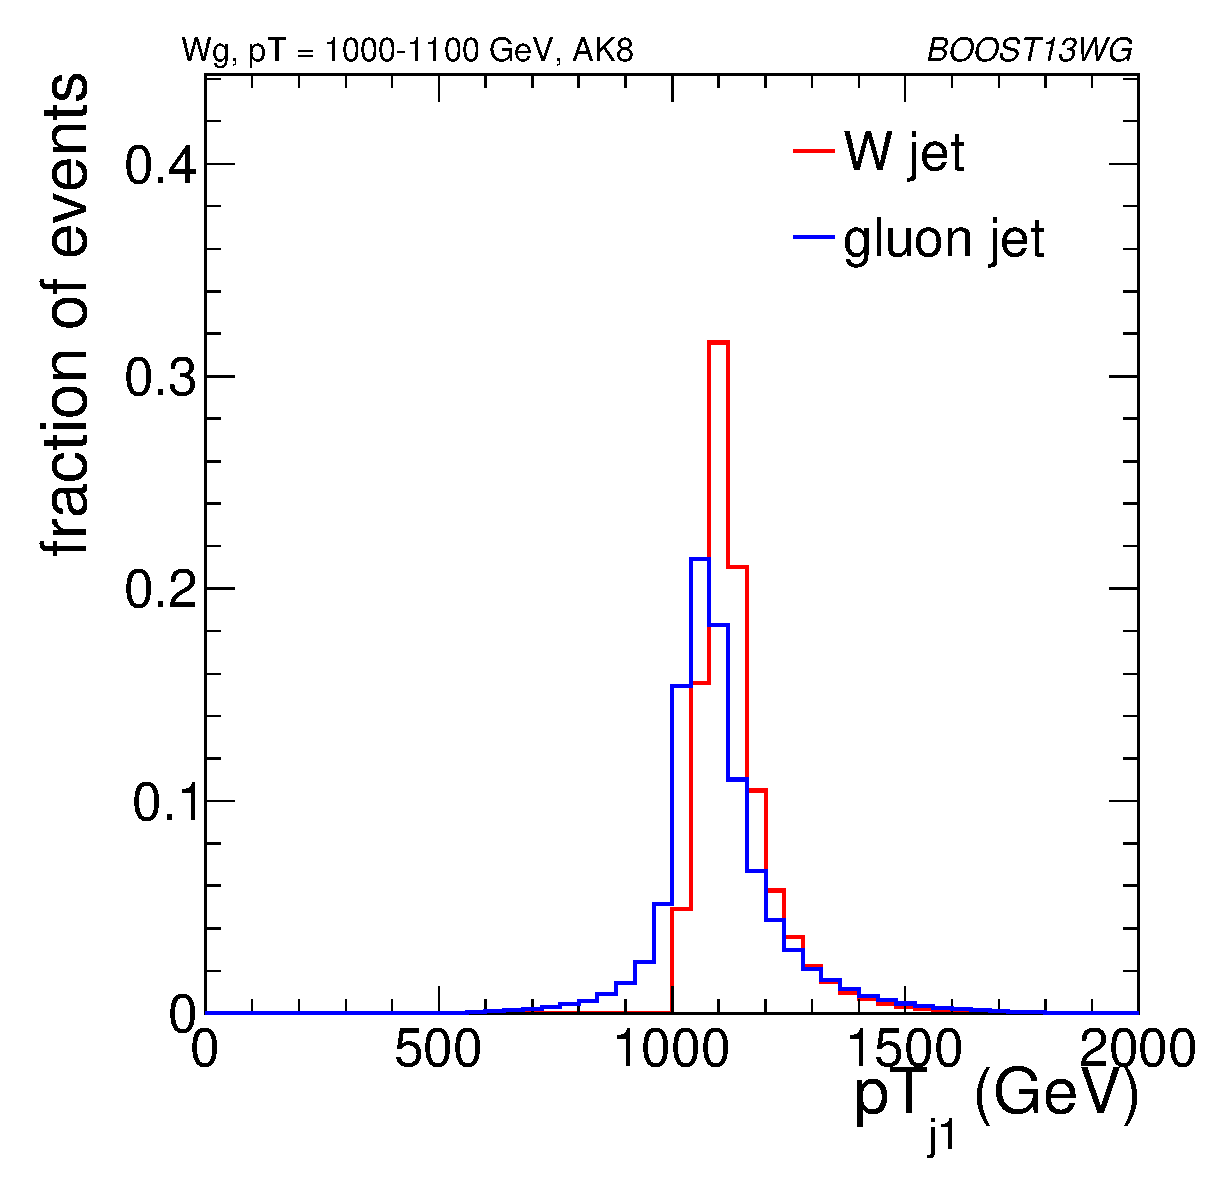
\includegraphics[width=0.30\textwidth]{./Figures/WTagging/pT1000/AKtR08/jpt1.eps}}
%\subfigure[\antikt R=1.2]{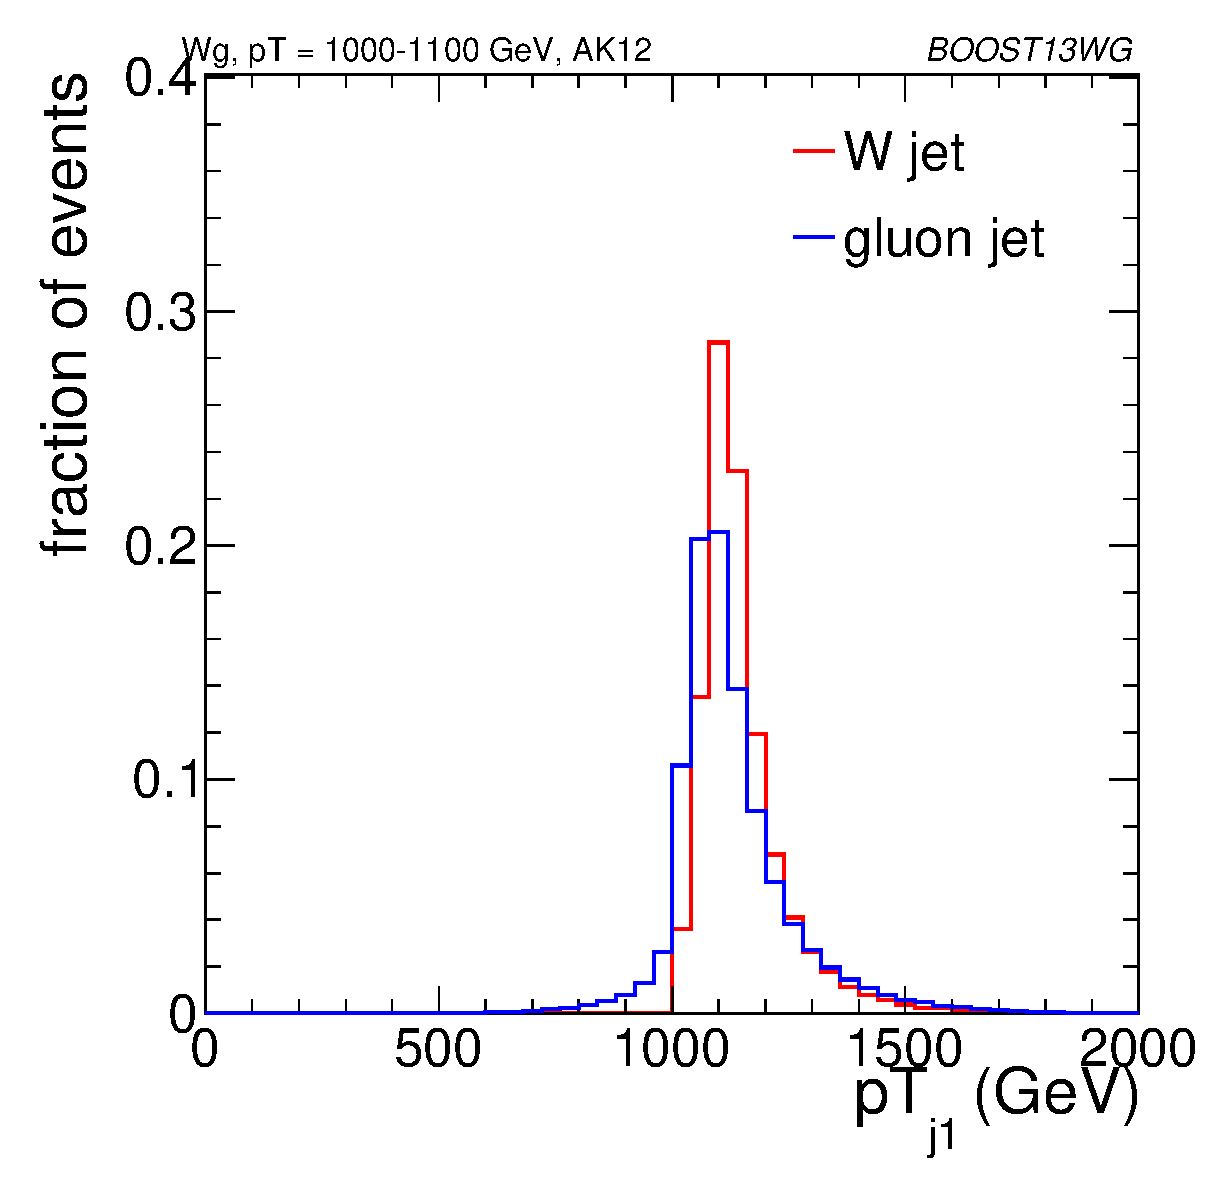
\includegraphics[width=0.30\textwidth]{./Figures/WTagging/pT1000/AKtR12/jpt1.eps}}
%\caption{Comparisons of the leading jet \pT spectrum of the $gg$
%  background to the WW signal in the \pT = 1.0-1.1 TeV bin using the
%  different \antikt jet distance parameters explored.}
%\label{fig:pt1000_basics}
%
%\end{figure*}



\subsection{Single Variable Performance}

In this section we  explore the performance of the various groomed
jet mass and substructure variables in separating signal
from background.
%, and how this performance changes depending on the
%kinematic bin and jet radius considered.
Since we
have not attempted to optimise the grooming parameter settings of
each grooming algorithm, we do not place much emphasis
here on the relative performance of the groomed masses, but instead
concentrate on how their performance changes depending on the
kinematic bin and jet radius considered. 

Figure~\ref{fig:pt500_mass_AKt_R08}  compares the signal and
background in terms of the different groomed masses explored for the
\antikt $R=0.8$ algorithm in the \pt = 500-600 \GeV bin. One can clearly see
that, in terms of separating signal and background, the groomed masses
are significantly more performant than the ungroomed \antikt $R=0.8$
mass. Using the same jet radius and \pt bin, Figure~\ref{fig:pt500_subst_AKt_R08}
compares signal and background for the different substructure variables
studied. 

\begin{figure*}
\centering
\subfigure[Ungroomed mass]{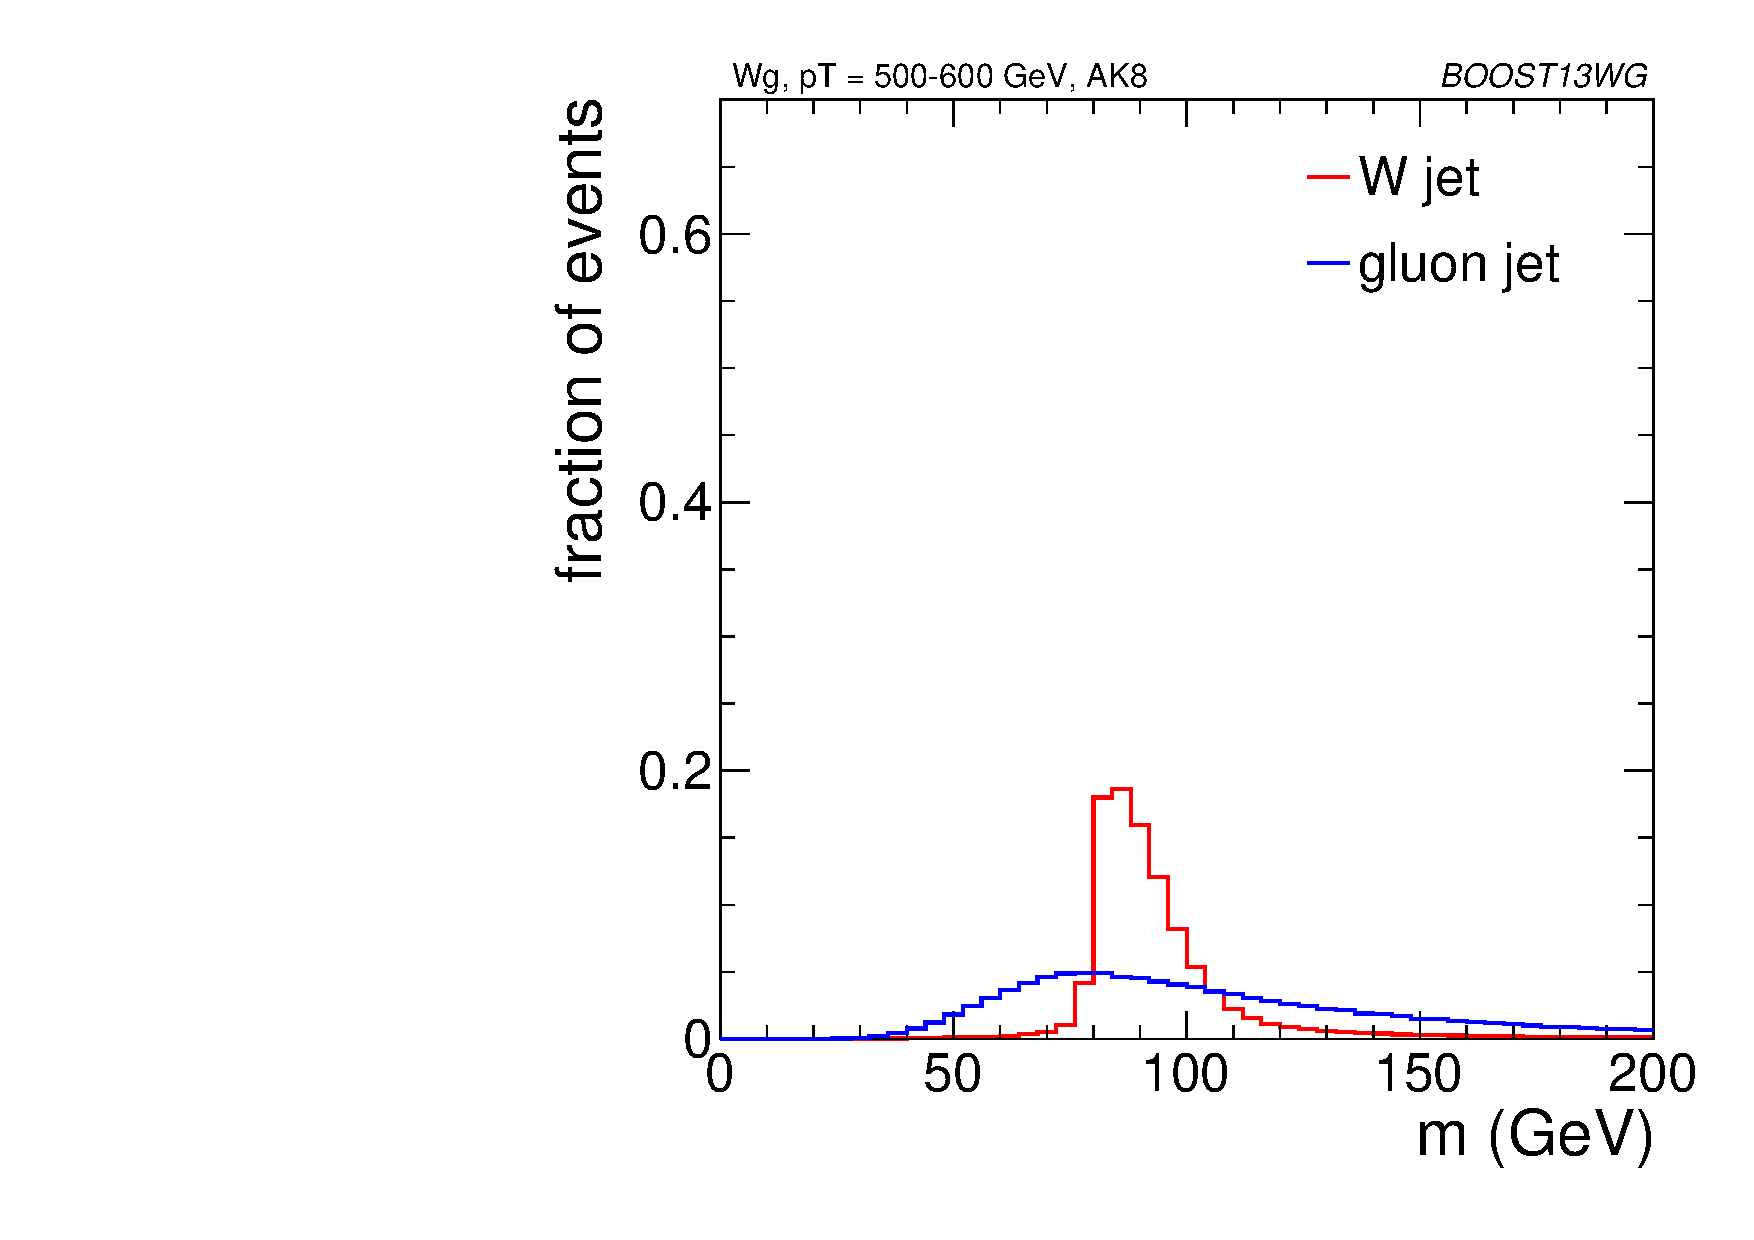
\includegraphics[width=0.30\textwidth]{./Figures/WTagging/pT500/AKtR08/jmass1.pdf}}
\subfigure[Pruned mass]{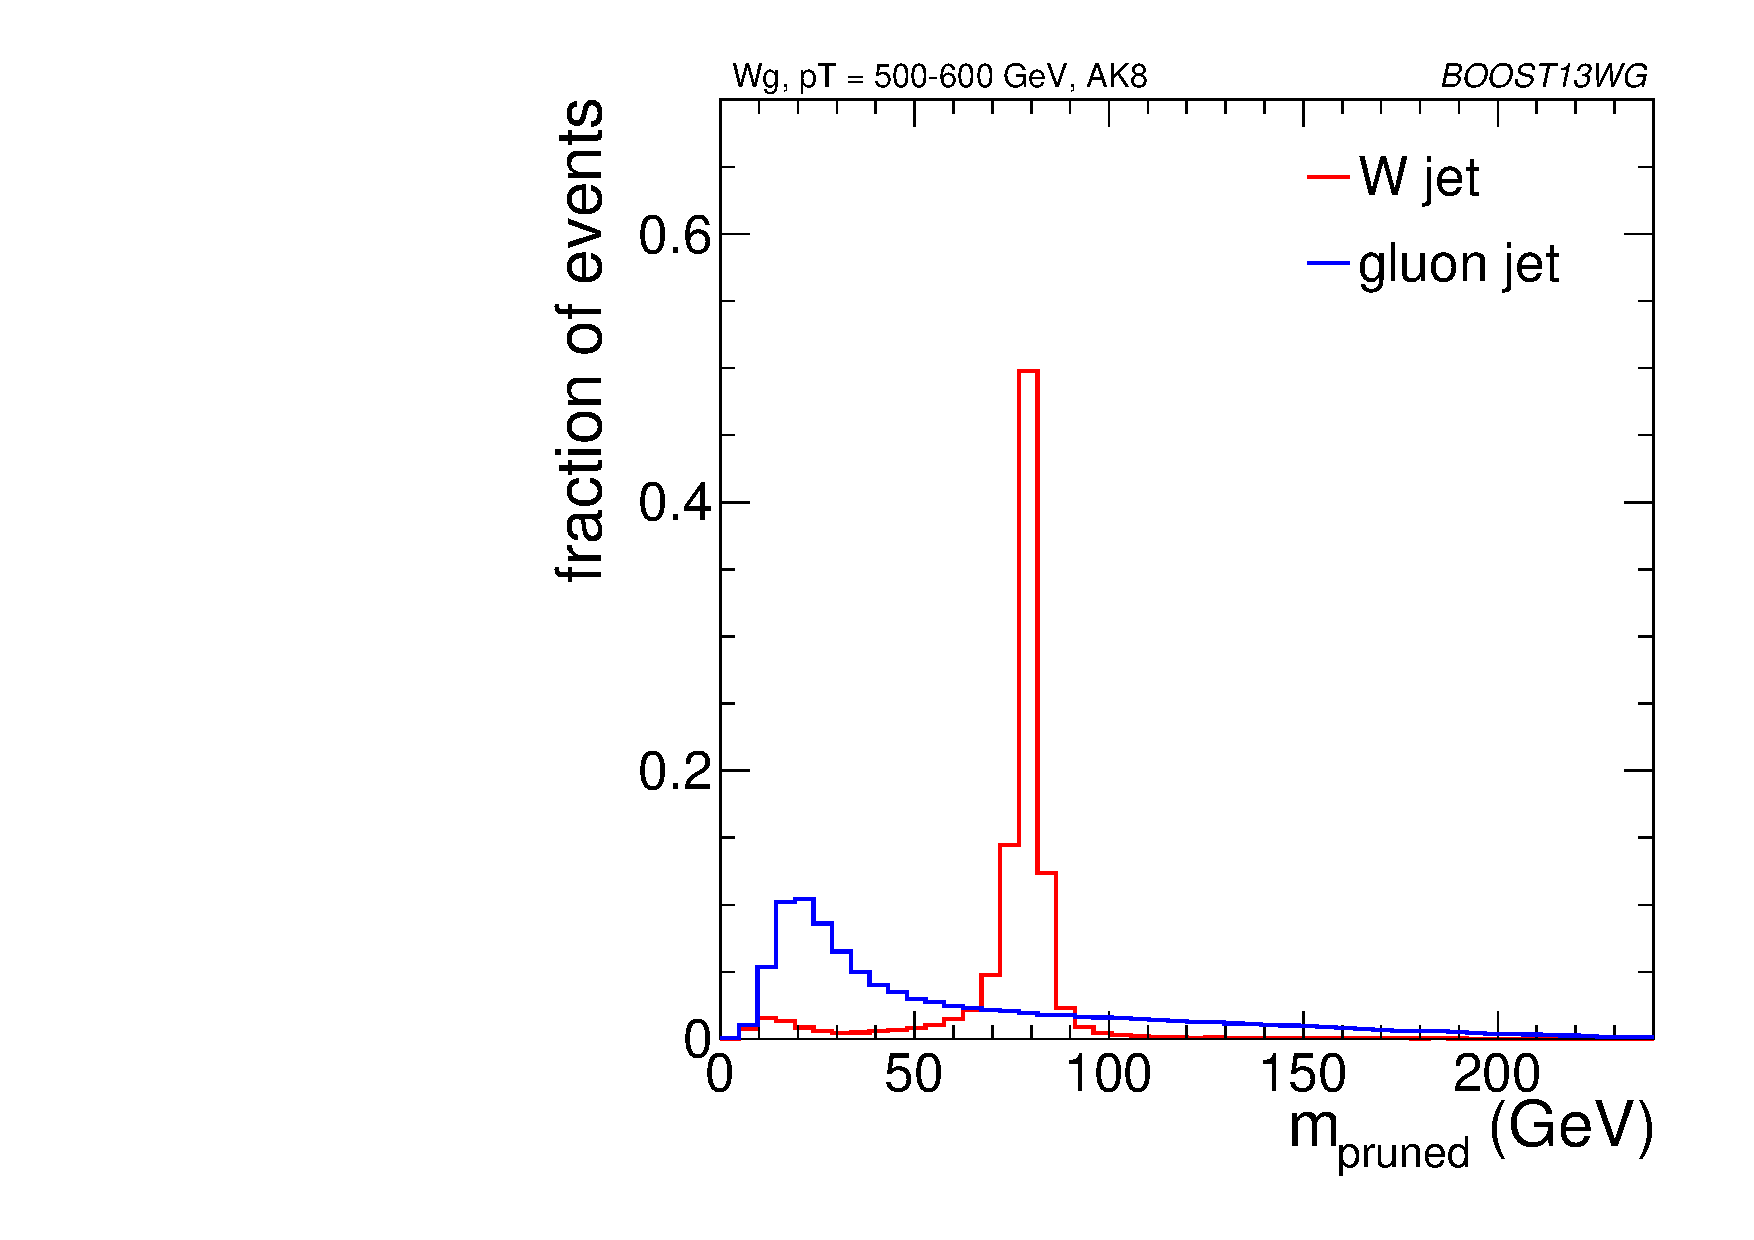
\includegraphics[width=0.30\textwidth]{./Figures/WTagging/pT500/AKtR08/h_mass_prun.pdf}}
\subfigure[Trimmed mass]{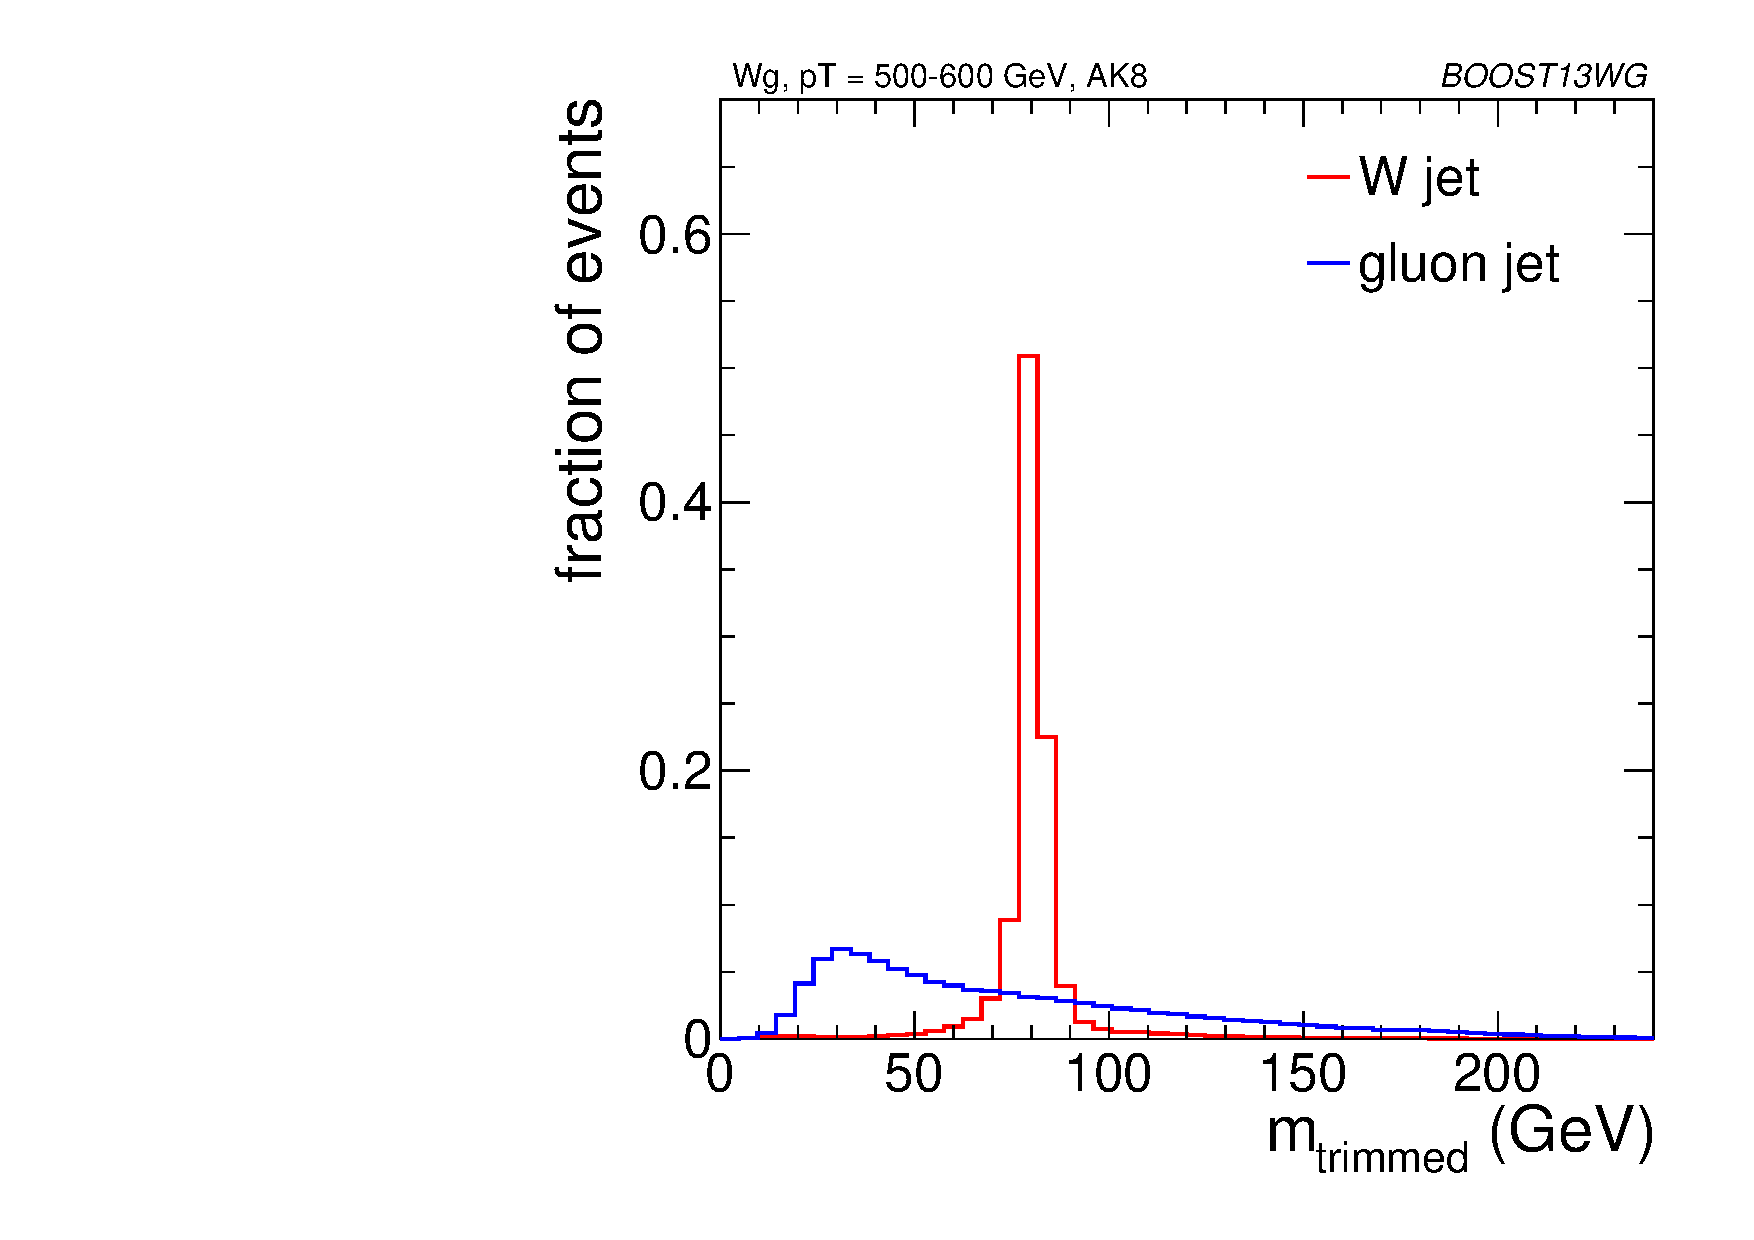
\includegraphics[width=0.30\textwidth]{./Figures/WTagging/pT500/AKtR08/h_mass_trim.pdf}}\\
\subfigure[mMDT mass]{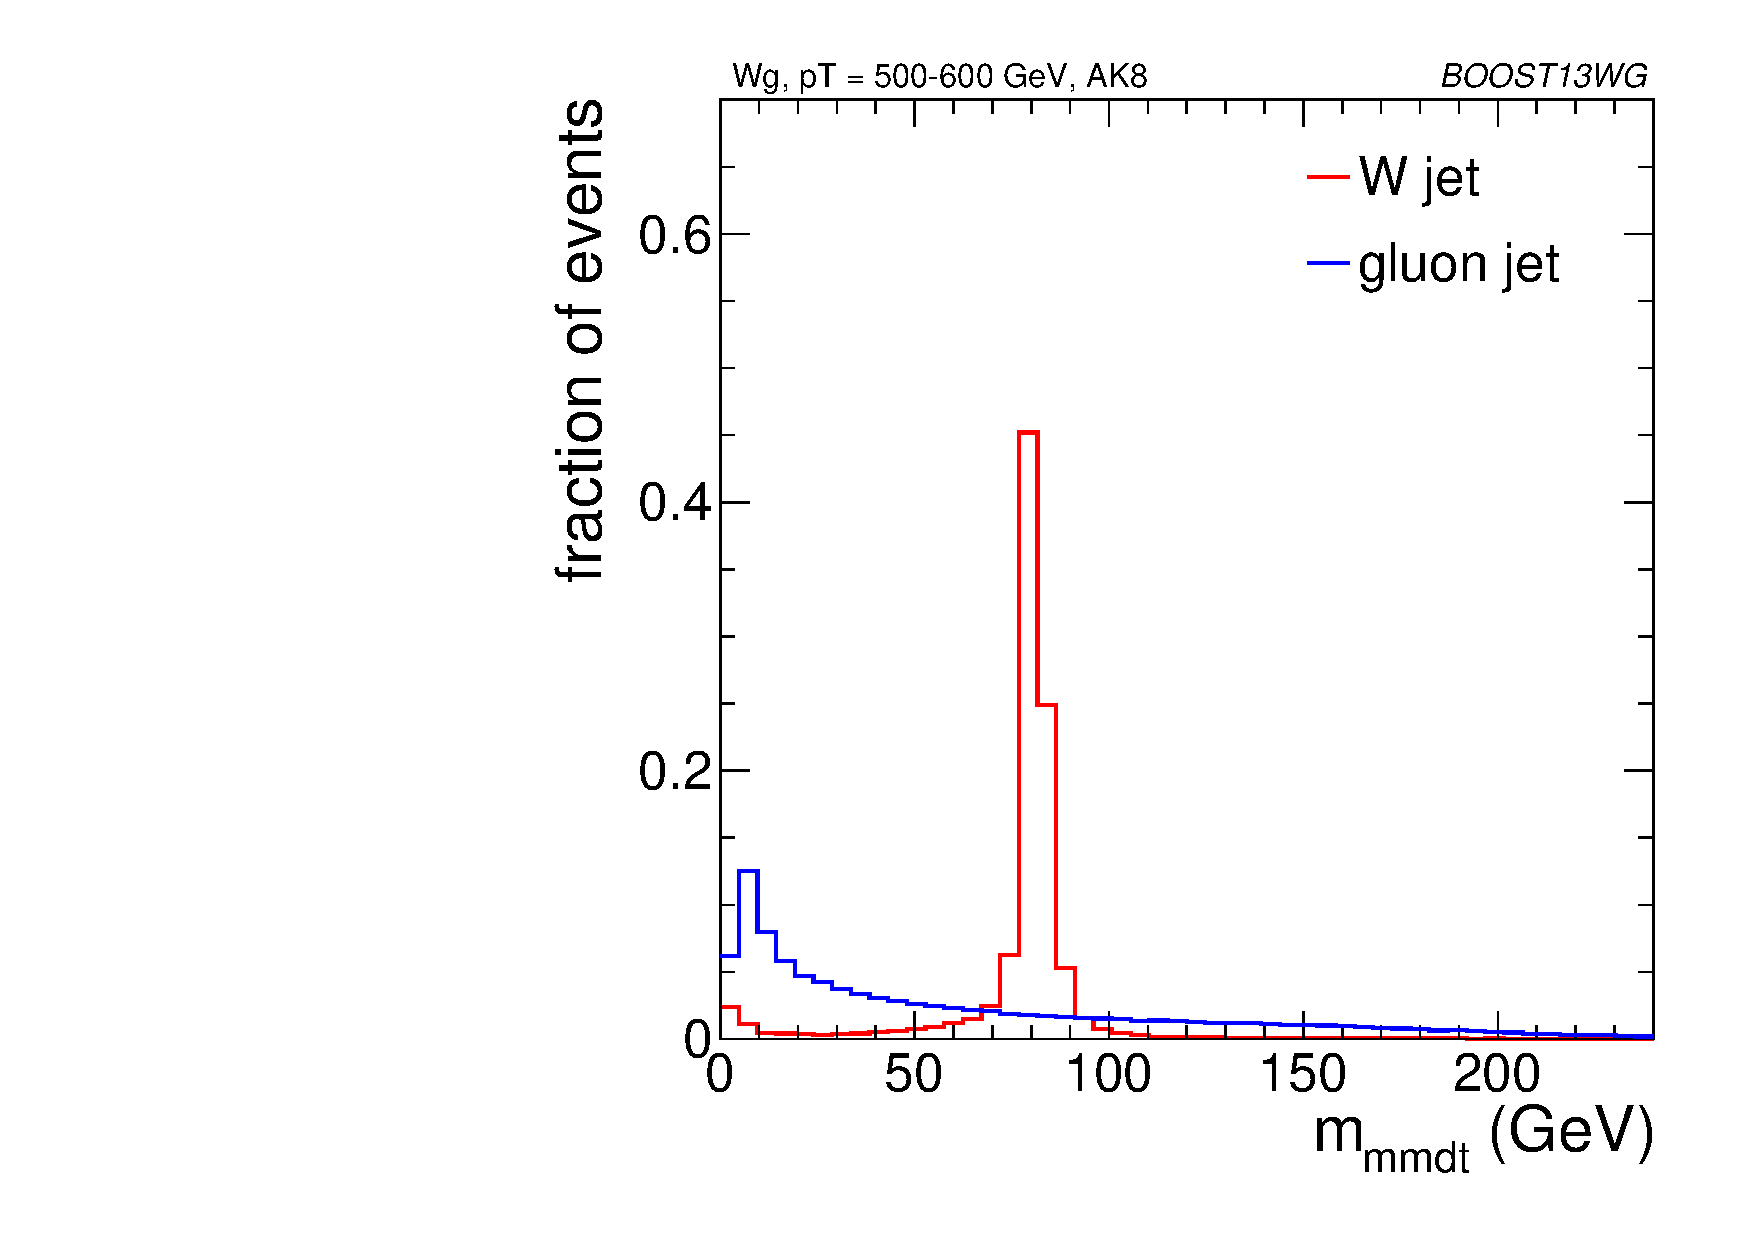
\includegraphics[width=0.30\textwidth]{./Figures/WTagging/pT500/AKtR08/h_mass_mmdt.pdf}}
\subfigure[Soft-drop $\beta=2$ mass]{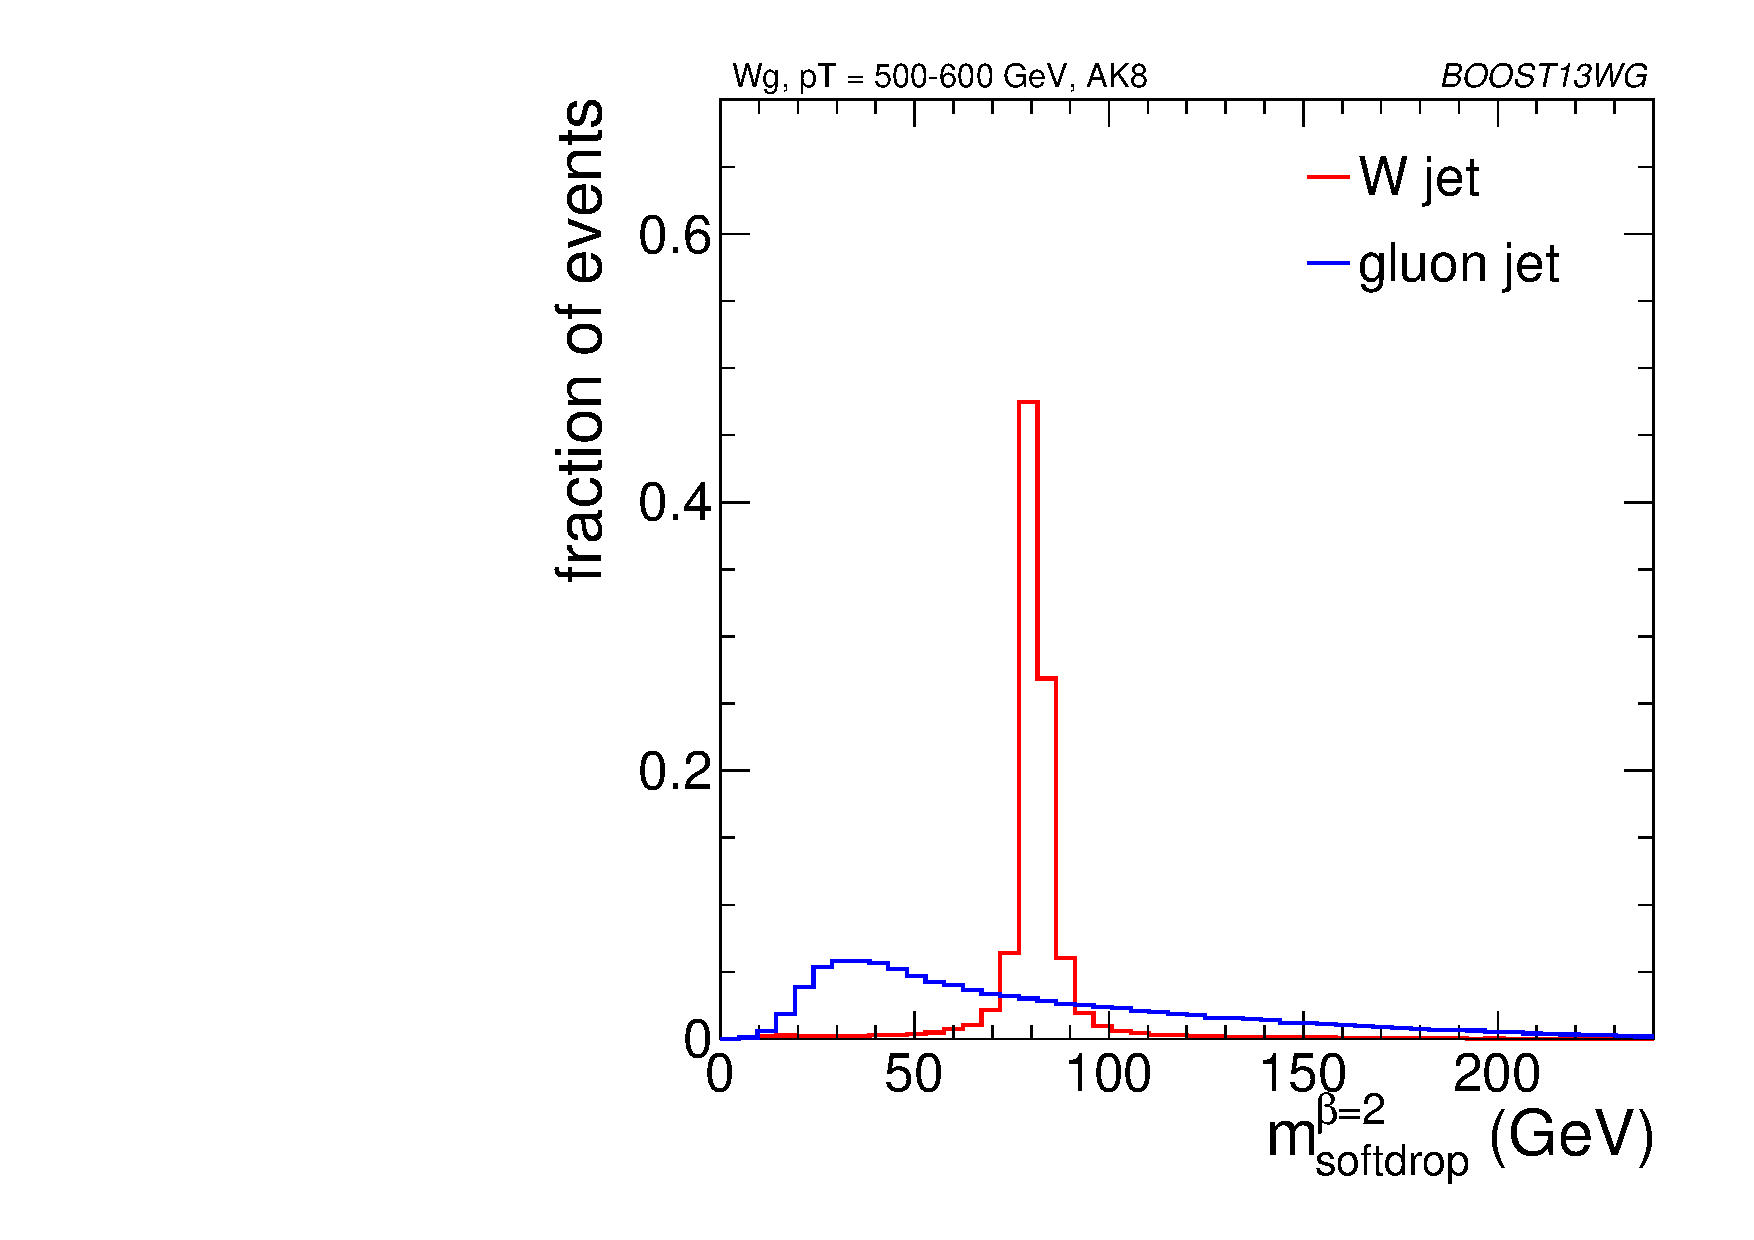
\includegraphics[width=0.30\textwidth]{./Figures/WTagging/pT500/AKtR08/h_mass_sdb2.pdf}}
%\subfigure[Soft-drop $\beta=-1$ mass]{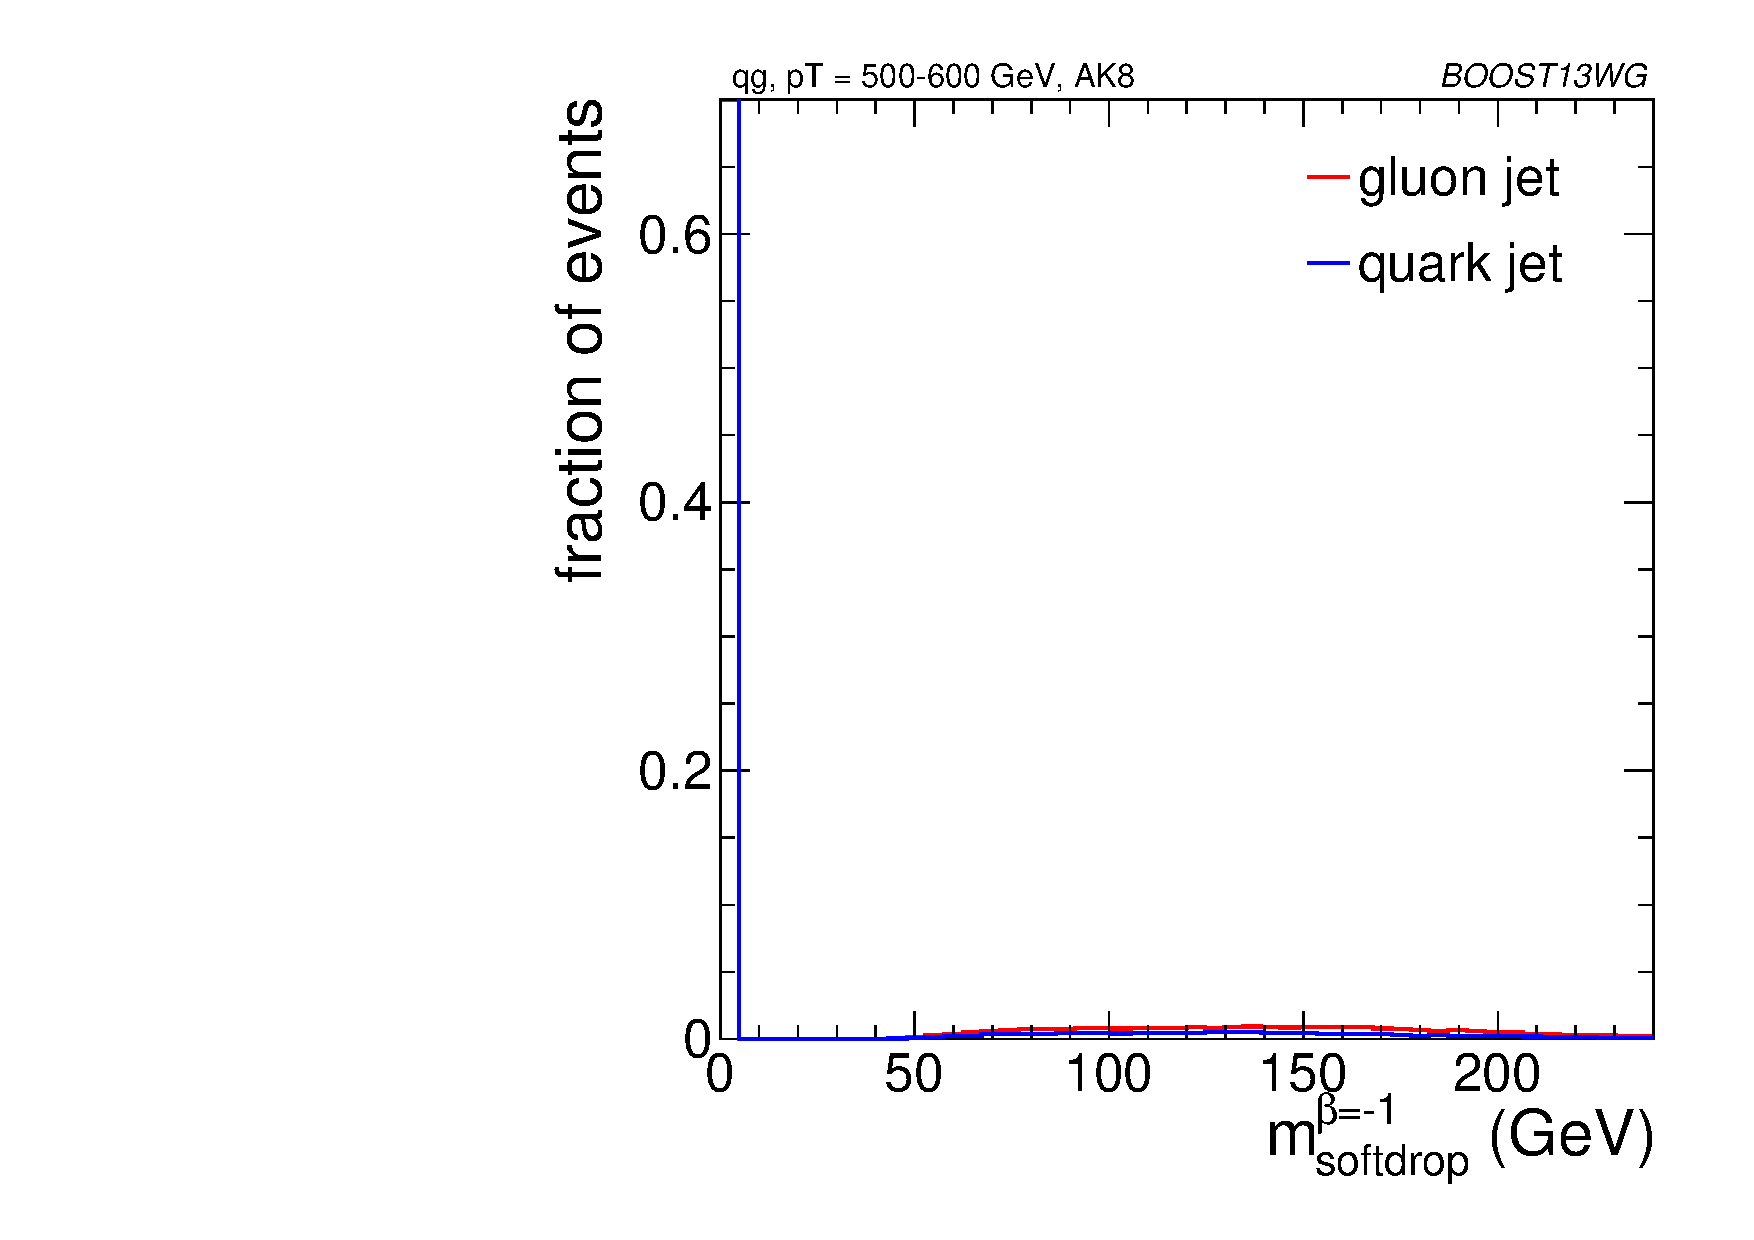
\includegraphics[width=0.48\textwidth]{./Figures/figs072514/figs071614_Wg_bin500_ak08/oneD/h_mass_sdm1.pdf}}
\caption{Leading jet mass distributions in the $gg$ background and
  $WW$ signal samples in the \pt = 500-600 \GeV bin using the \antikt $R=0.8$ algorithm.}
\label{fig:pt500_mass_AKt_R08}
\end{figure*}

\begin{figure*}
\centering
\subfigure[$C_2^{\beta=1}$]{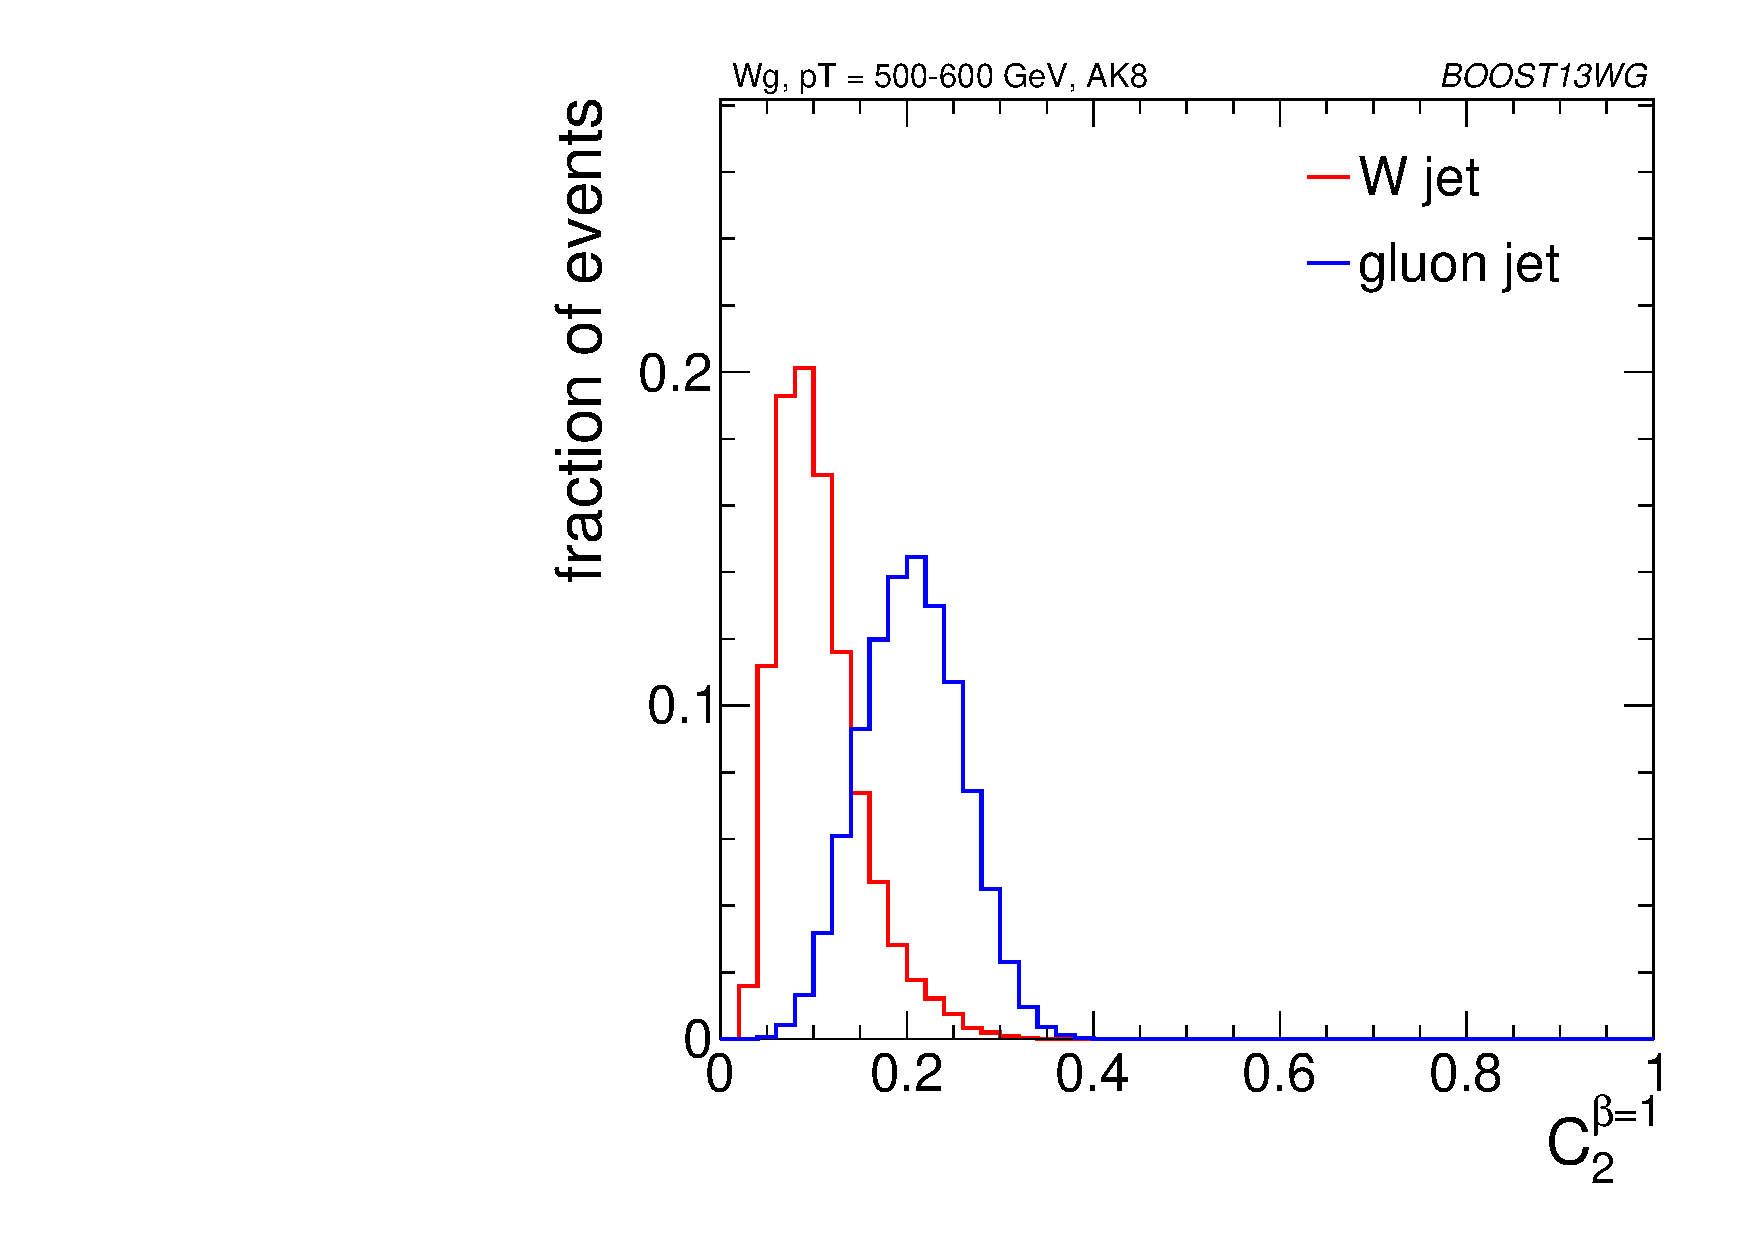
\includegraphics[width=0.30\textwidth]{./Figures/WTagging/pT500/AKtR08/h_c2_b1.pdf}}
\subfigure[$C_2^{\beta=2}$]{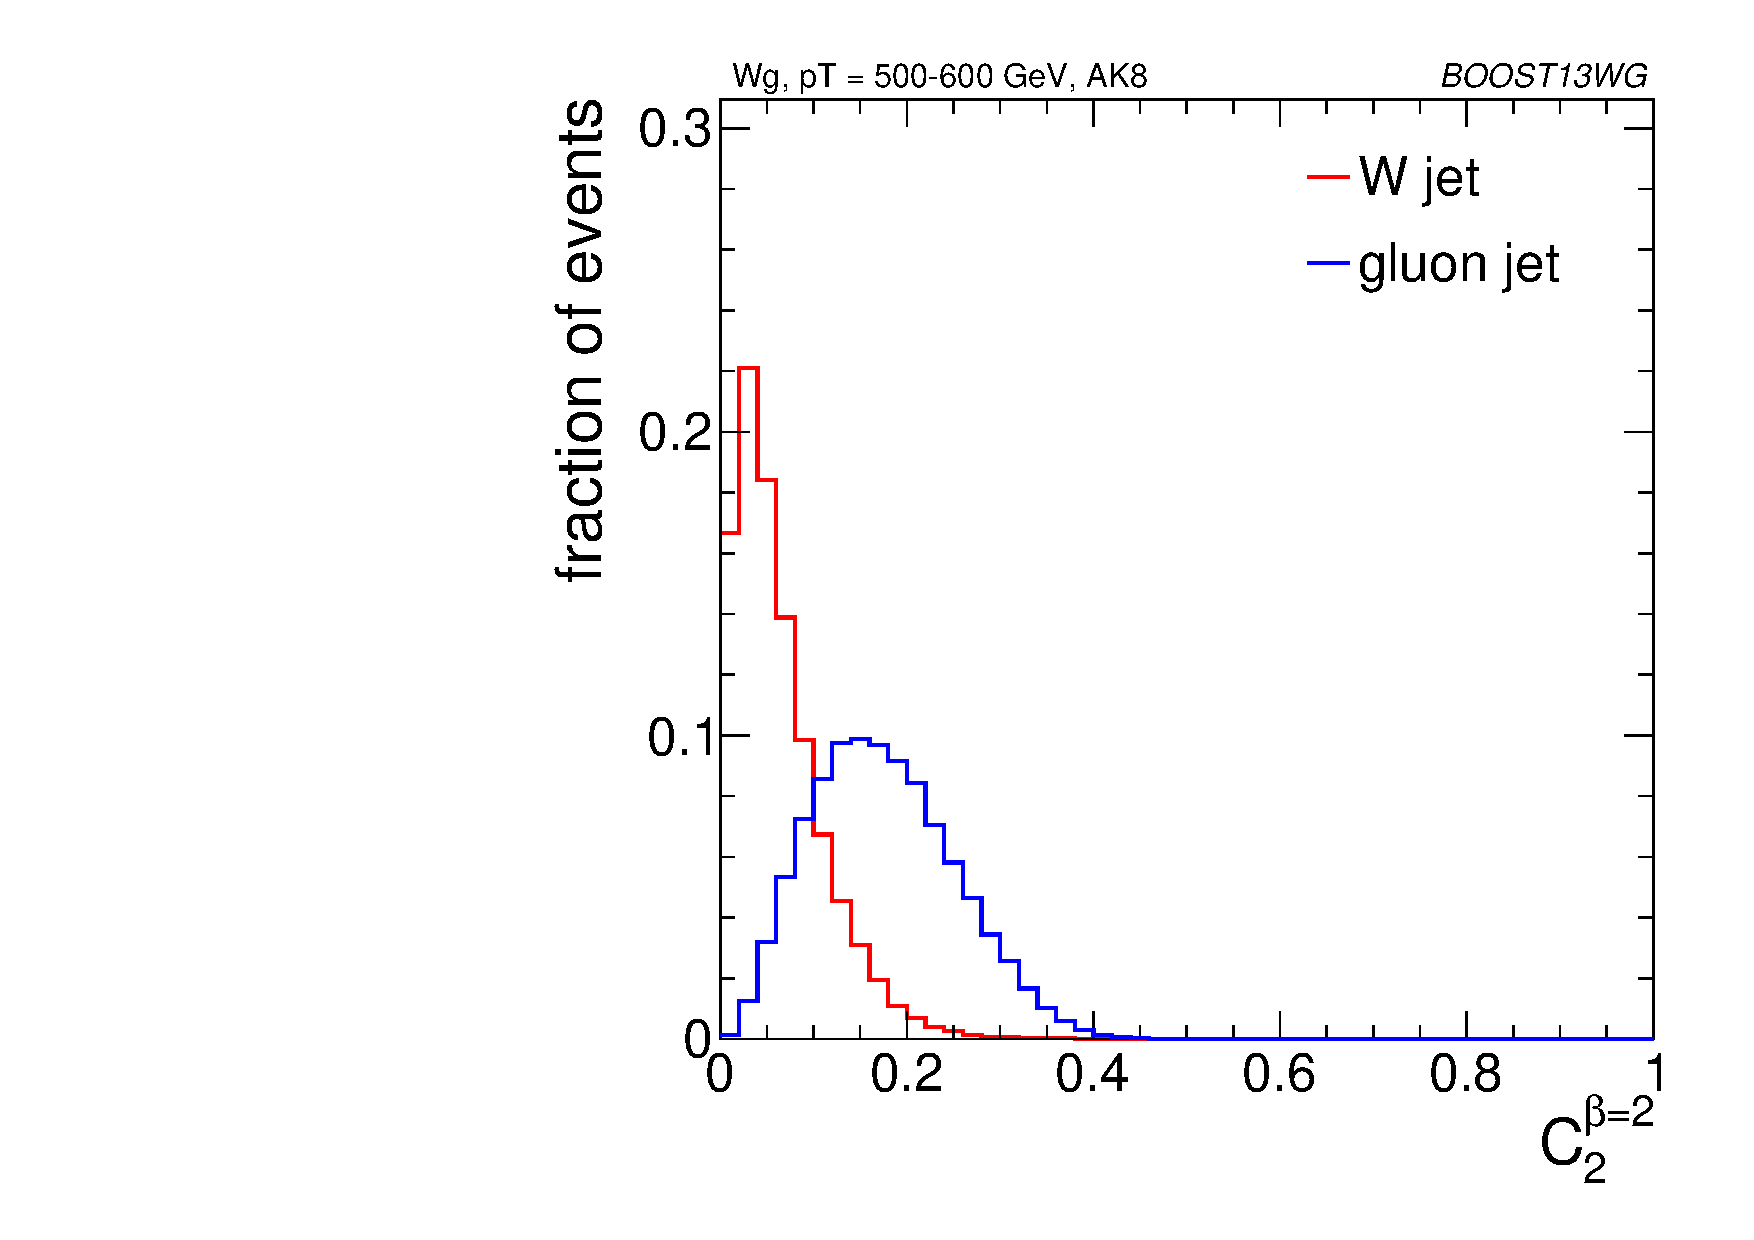
\includegraphics[width=0.30\textwidth]{./Figures/WTagging/pT500/AKtR08/h_c2_b2.pdf}}
\subfigure[$\Gamma_{Qjet}$]{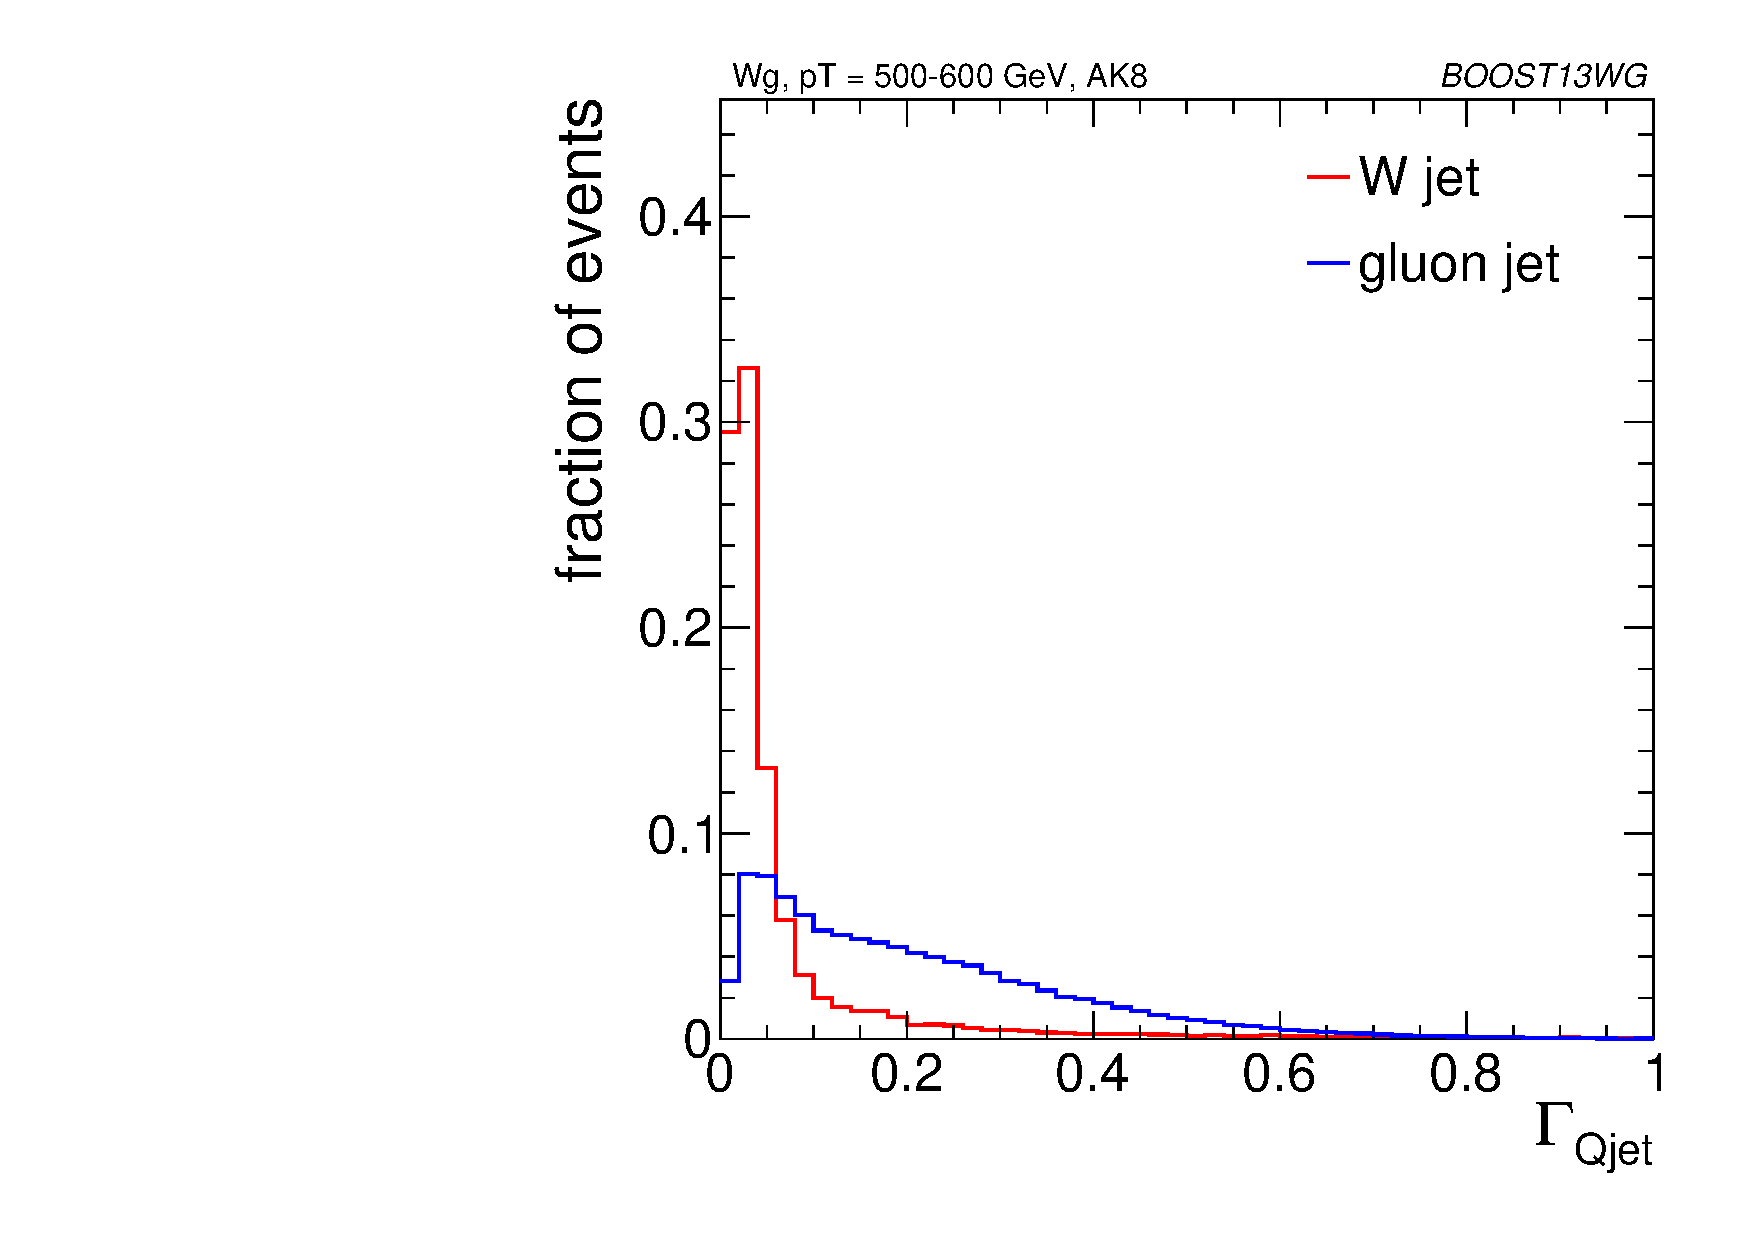
\includegraphics[width=0.30\textwidth]{./Figures/WTagging/pT500/AKtR08/h_qjetVol.pdf}}\\
\subfigure[$\tau_{21}^{\beta=1}$]{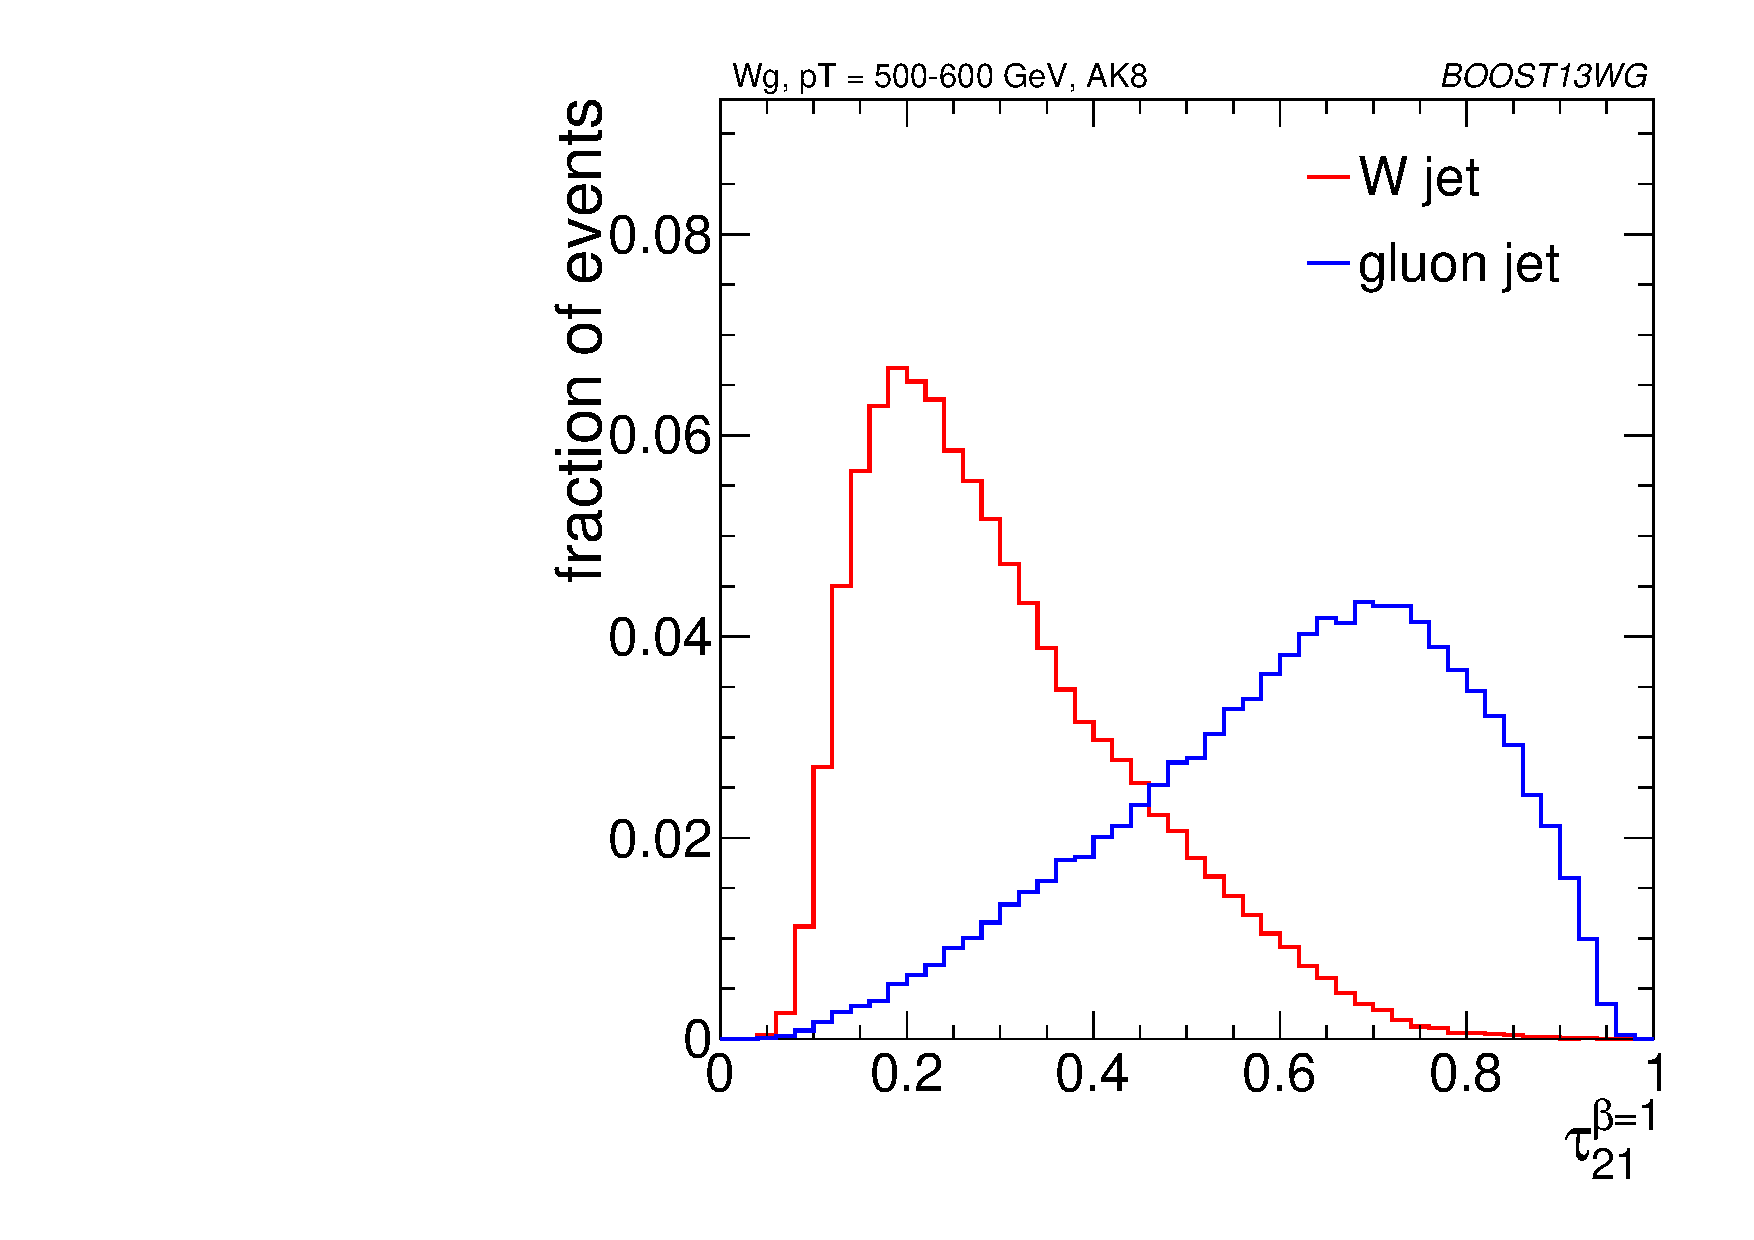
\includegraphics[width=0.30\textwidth]{./Figures/WTagging/pT500/AKtR08/h_tau21_b1.pdf}}
\subfigure[$\tau_{21}^{\beta=2}$]{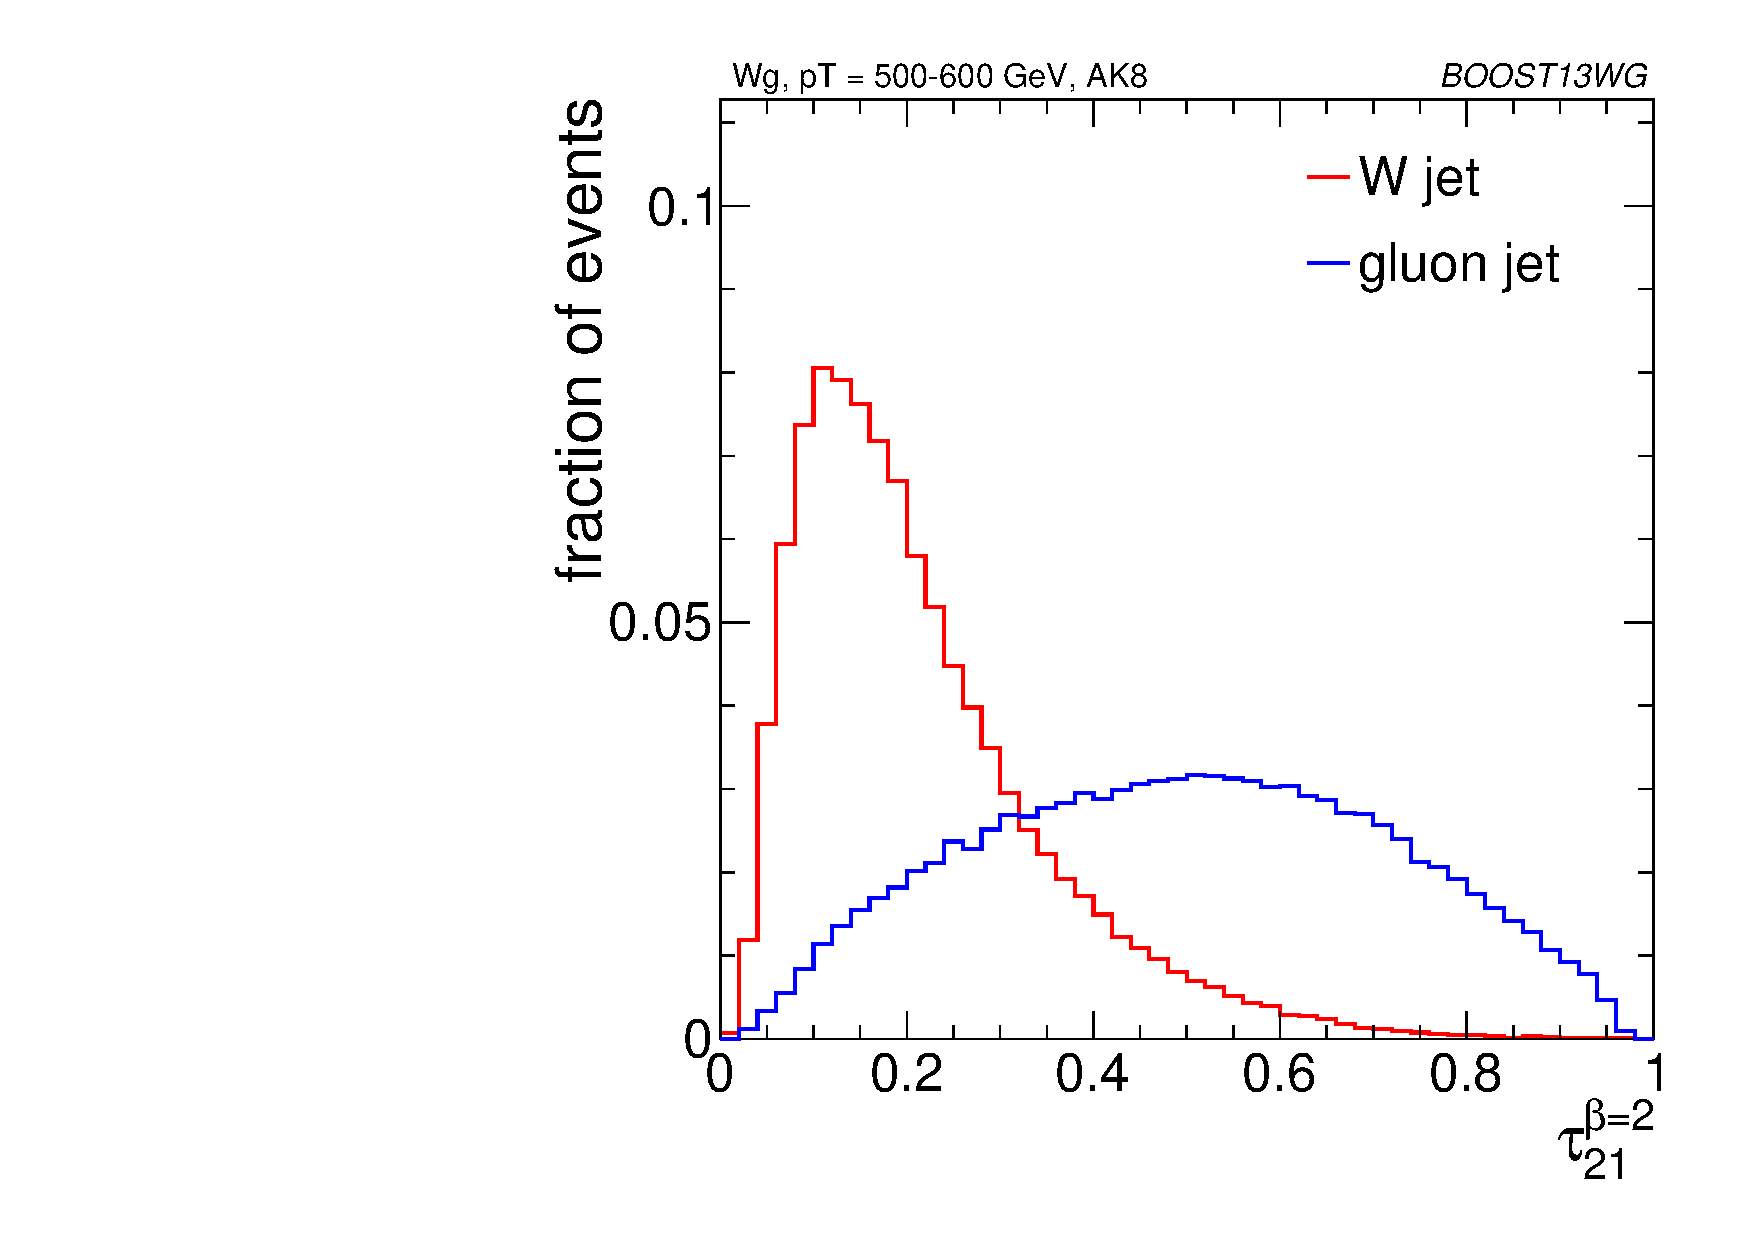
\includegraphics[width=0.30\textwidth]{./Figures/WTagging/pT500/AKtR08/h_tau21_b2.pdf}}
\caption{Leading jet substructure variable distributions in the $gg$
  background and $WW$ signal samples in the \pt = 500-600 \GeV bin using the \antikt $R=0.8$ algorithm.}
\label{fig:pt500_subst_AKt_R08}
\end{figure*}


Figures~\ref{fig:pt300_single},~\ref{fig:pt500_single}
and~\ref{fig:pt1000_single} show the single variable ROC curves
for various \pt bins and values of $R$. The single variable performance is also
compared to the ROC curve for a BDT combination of all the variables
(labelled ``allvars''). In all cases, the ``allvars'' option
is significantly more performant than any of the individual single variables
considered, indicating that there is considerable complementarity
between the variables, and this is explored further in Section~\ref{sec:w_combined}.

%Comparing the impact of increasing the jet
%radius in the same kinematic bin, one can see that the groomed mass
%performance does not vary greatly, but that the performance of the
%substructure variables is markedly worse for larger jet radius.



%At low pT, substructure performance gets worse across the board as radius increases
%In Figure~\ref{fig:pt500_comb2D}  we can also
%observe that the degradation of the substructure variable performance
%with increased jet radius is not uniform. The background rejection of
%$C_2^{\beta=1}$ degrades substantially more than that of
%$\tau_{21}^{\beta=1}$ as the 
%At highest pT, the situation is different again....

% when you are at the characteristic scale of the jet, C2B1 does well,
% but when it is wider than necessaruy it starts to fail

%Figure~\ref{fig:pt500_single_AKt_R08} shows the single variable ROC curves in
%the \pT = 500 GeV bin for the anti-\kT R=0.8 algorithm, compared to the
%ROC curve for a BDT combination of all the variables. One can see that
%the best performant single variables for a reasonable signal
%efficiency are the groomed/filtered masses, which all have a similar
%level of performance with the exception of the soft drop mass with $\beta=-1$. {\it Would be good to split this into two plots, one
%using the masses and one for other variables, or somehow make the mass
%and other variable curves more distinct from one another by using same
%colour for all the mass curves}.
%
%{\it We want to look also at:
%\begin{itemize}
%\item Dependence on R. So have the same single variable ROC for
%e.g. R=1.2, R=0.4. Then possibly have another plot which compares the
%best single variable (e.g. groomed mass) for
%different R.
%\item Dependence on pT. Again want to repeat the plot for different
%kinematic bins, and then have a plot which compares the best
%performance in each kinematic bin to see the dependence of performance
%on kinematics.
%\end{itemize}
%}

\begin{figure*}
\centering
\subfigure[\antikt $R=0.8$, \pt = 300-400 \GeV bin]{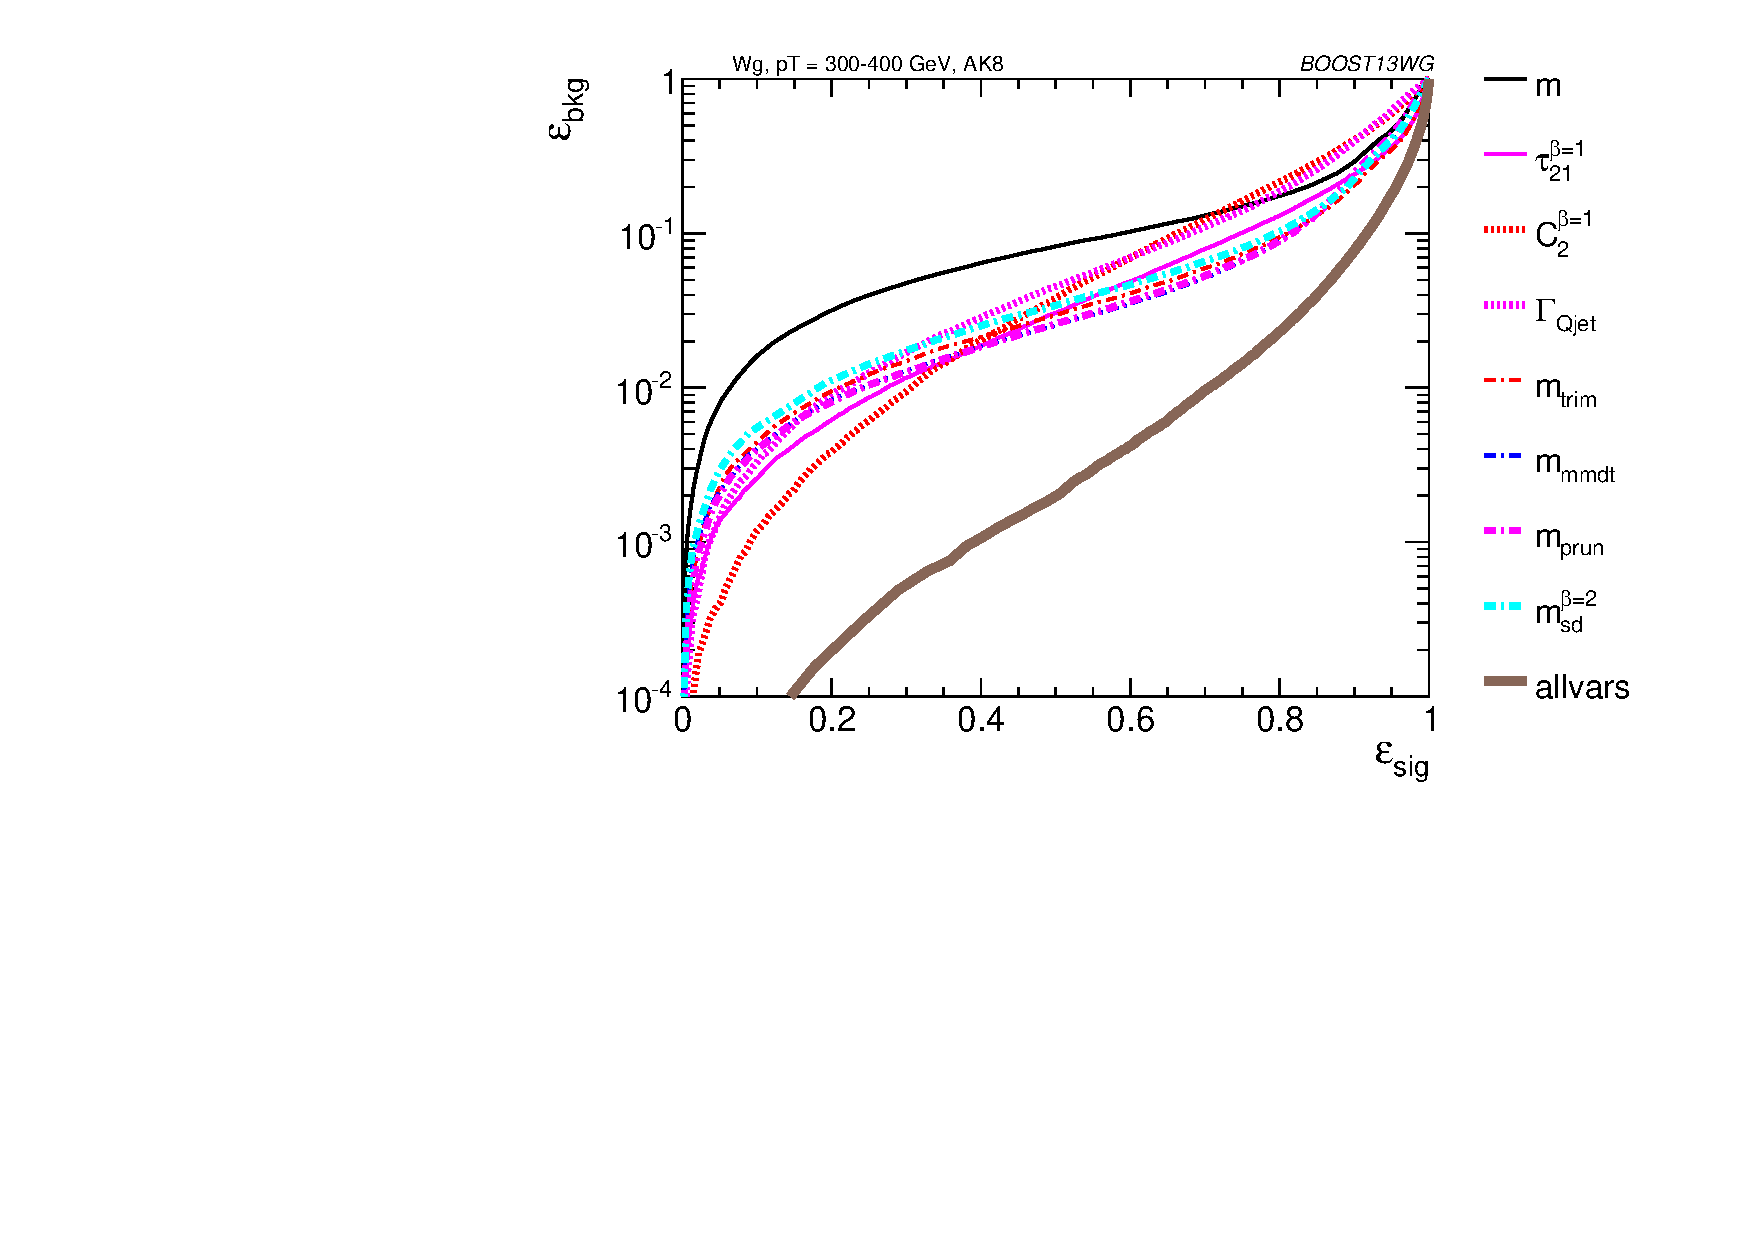
\includegraphics[width=0.48\textwidth]{./Figures/WTagging/pT300/AKtR08/Rocs_1D_single.pdf}}
\subfigure[\antikt $R=1.2$, \pt = 300-400 \GeV bin]{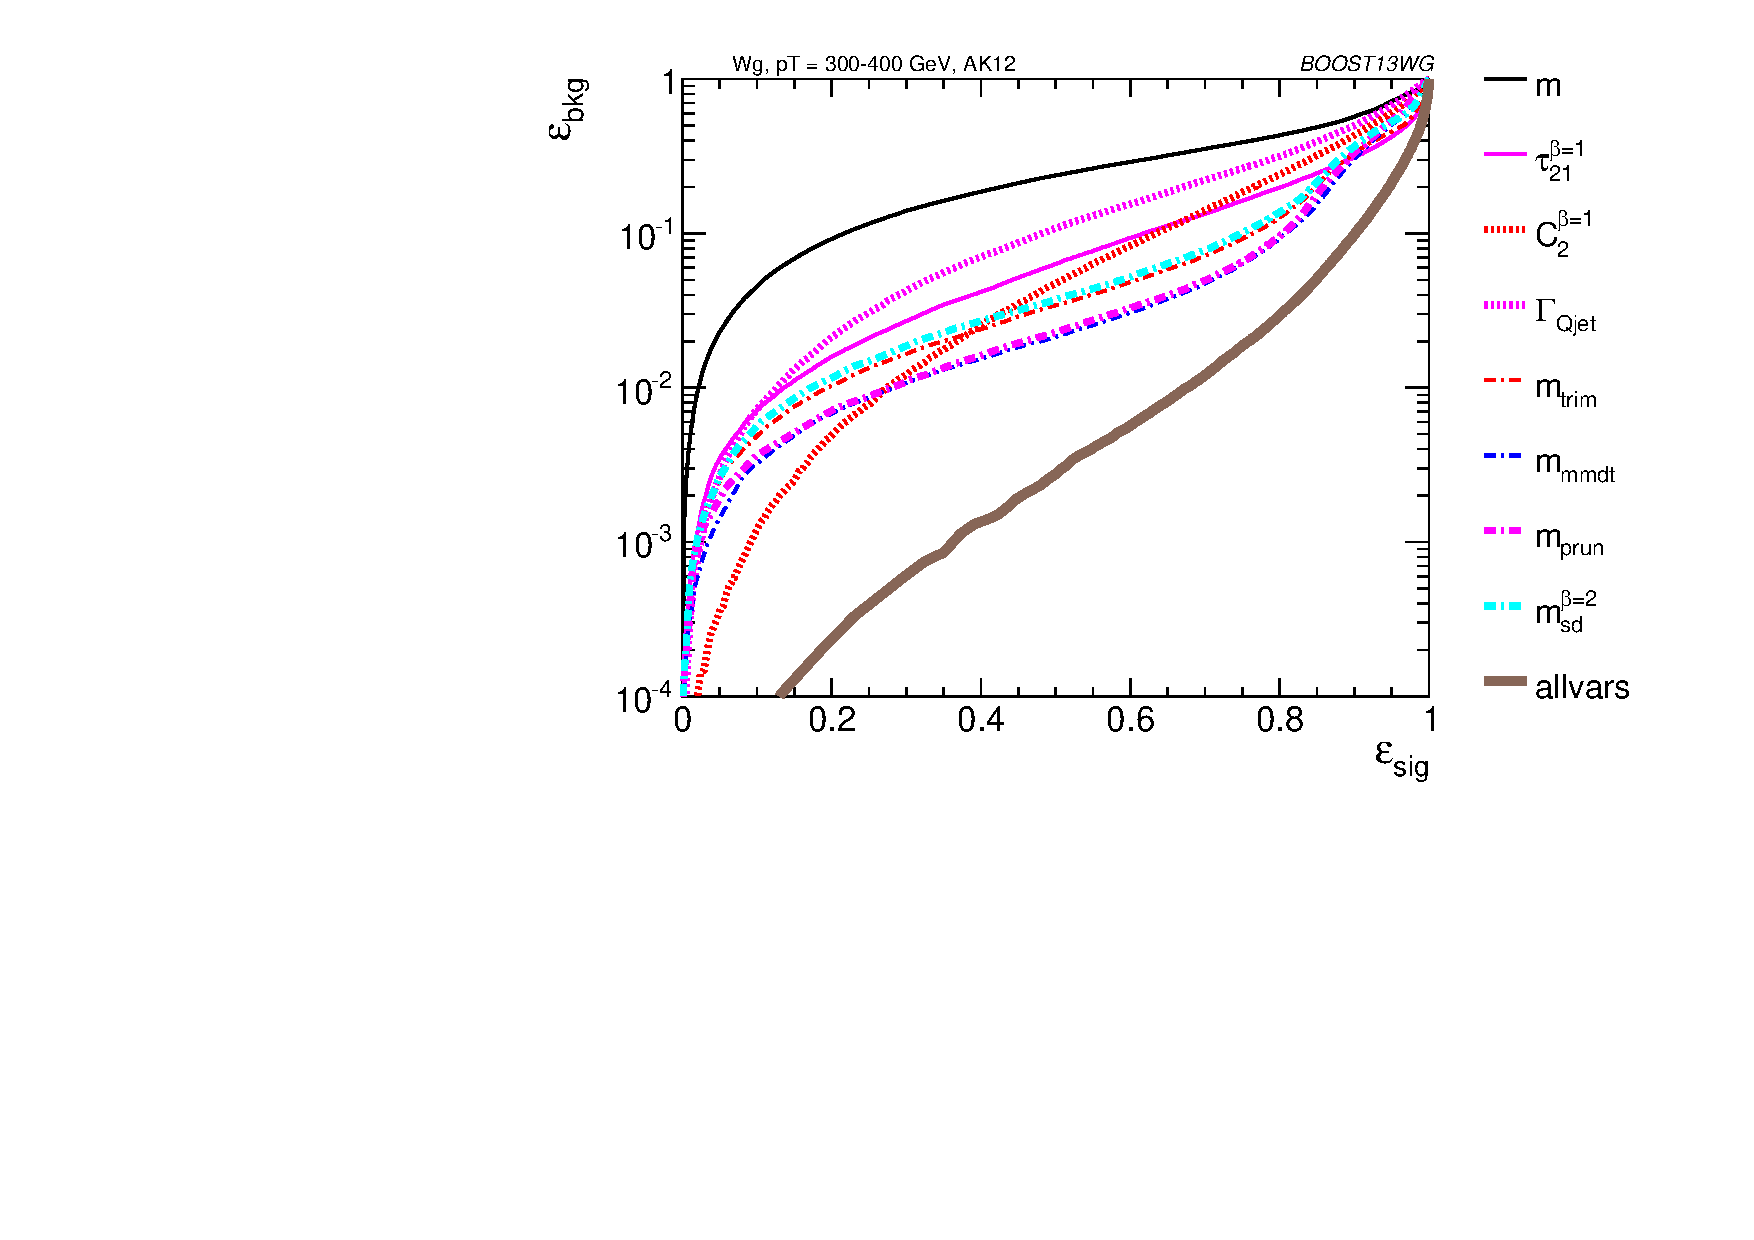
\includegraphics[width=0.48\textwidth]{./Figures/WTagging/pT300/AKtR12/Rocs_1D_single.pdf}}
\caption{ROC curves for single variables considered for $W$
tagging in the \pt = 300-400 \GeV bin using the \antikt $R=0.8$ algorithm and $R=1.2$ algorithm, along with a BDT combination of all variables (``allvars'').}
\label{fig:pt300_single}
\end{figure*}


\begin{figure*}
\centering
\subfigure[\antikt $R=0.8$, \pt = 500-600 \GeV bin]{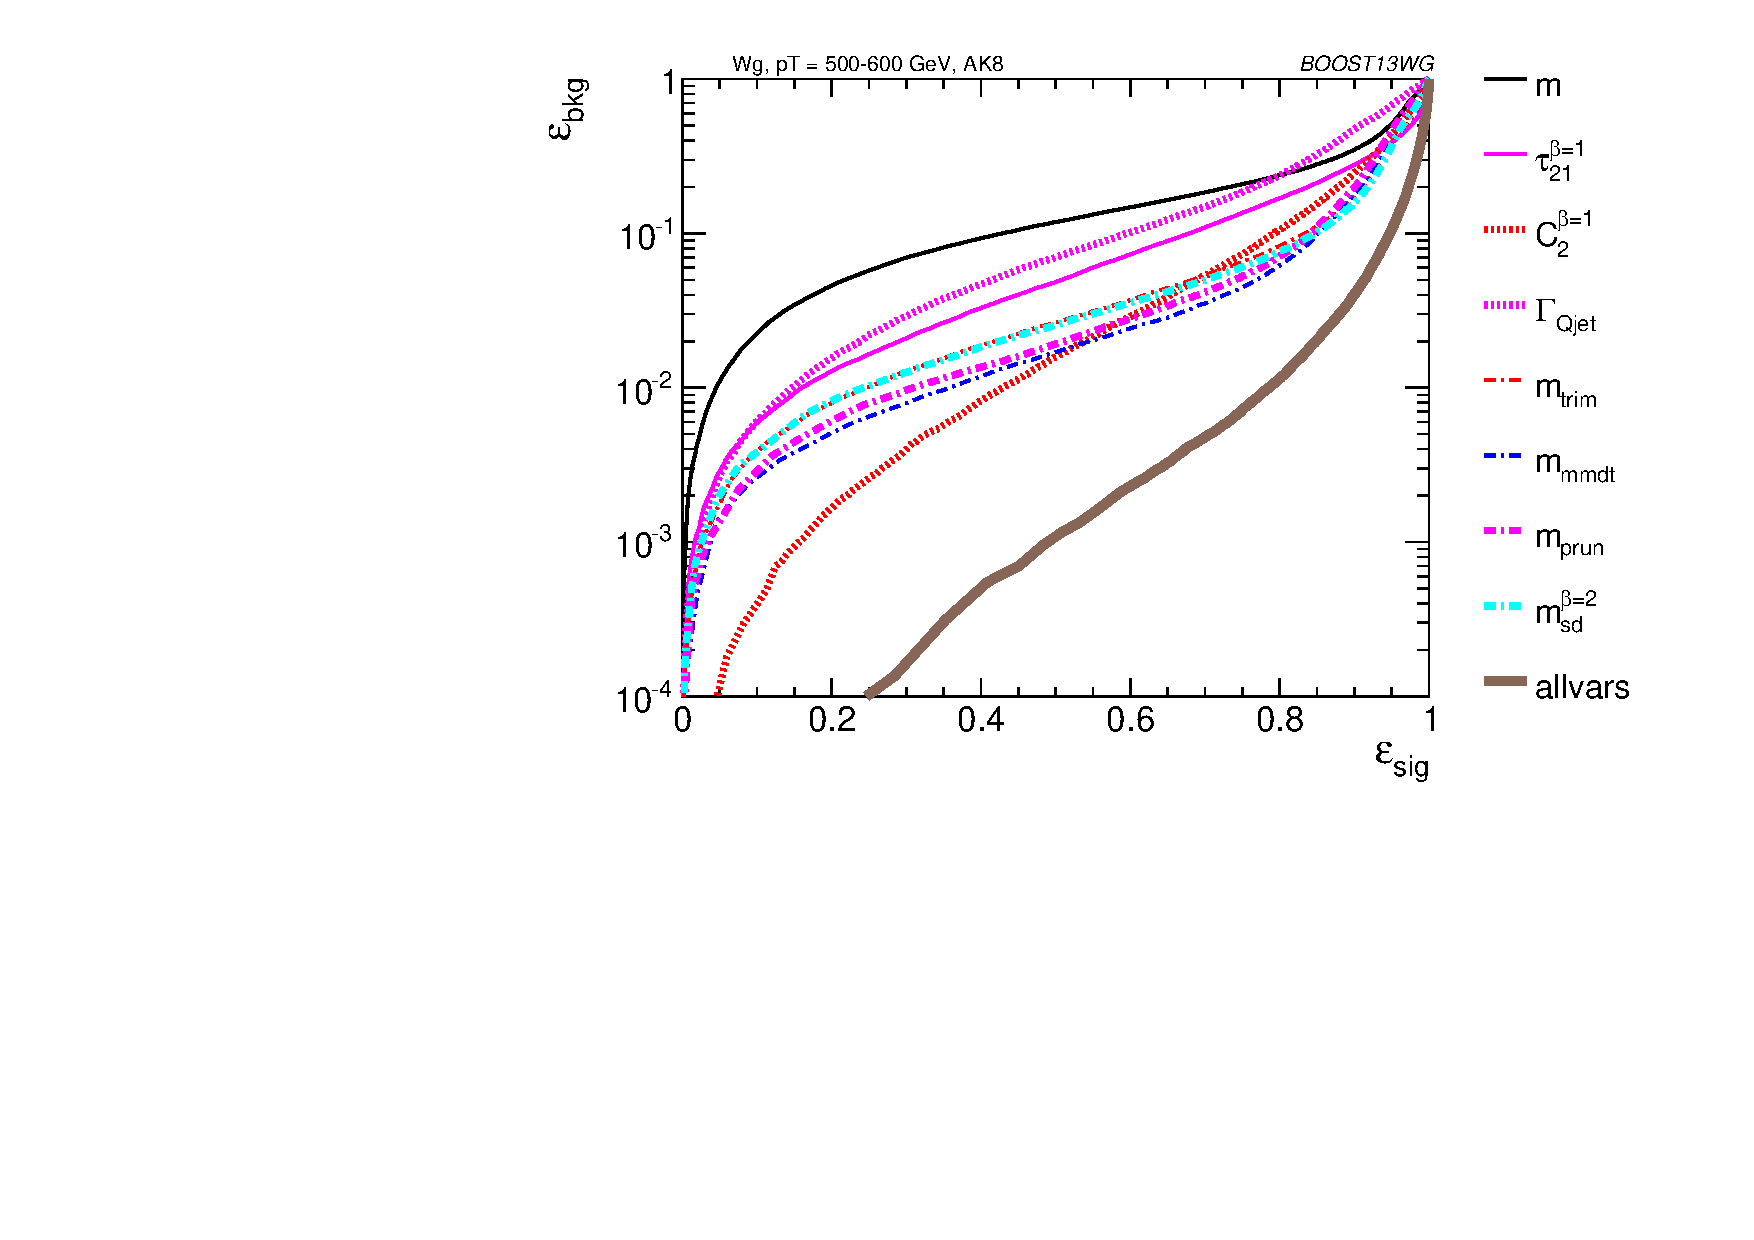
\includegraphics[width=0.48\textwidth]{./Figures/WTagging/pT500/AKtR08/Rocs_1D_single.pdf}}
\subfigure[\antikt $R=1.2$, \pt = 500-600 \GeV bin]{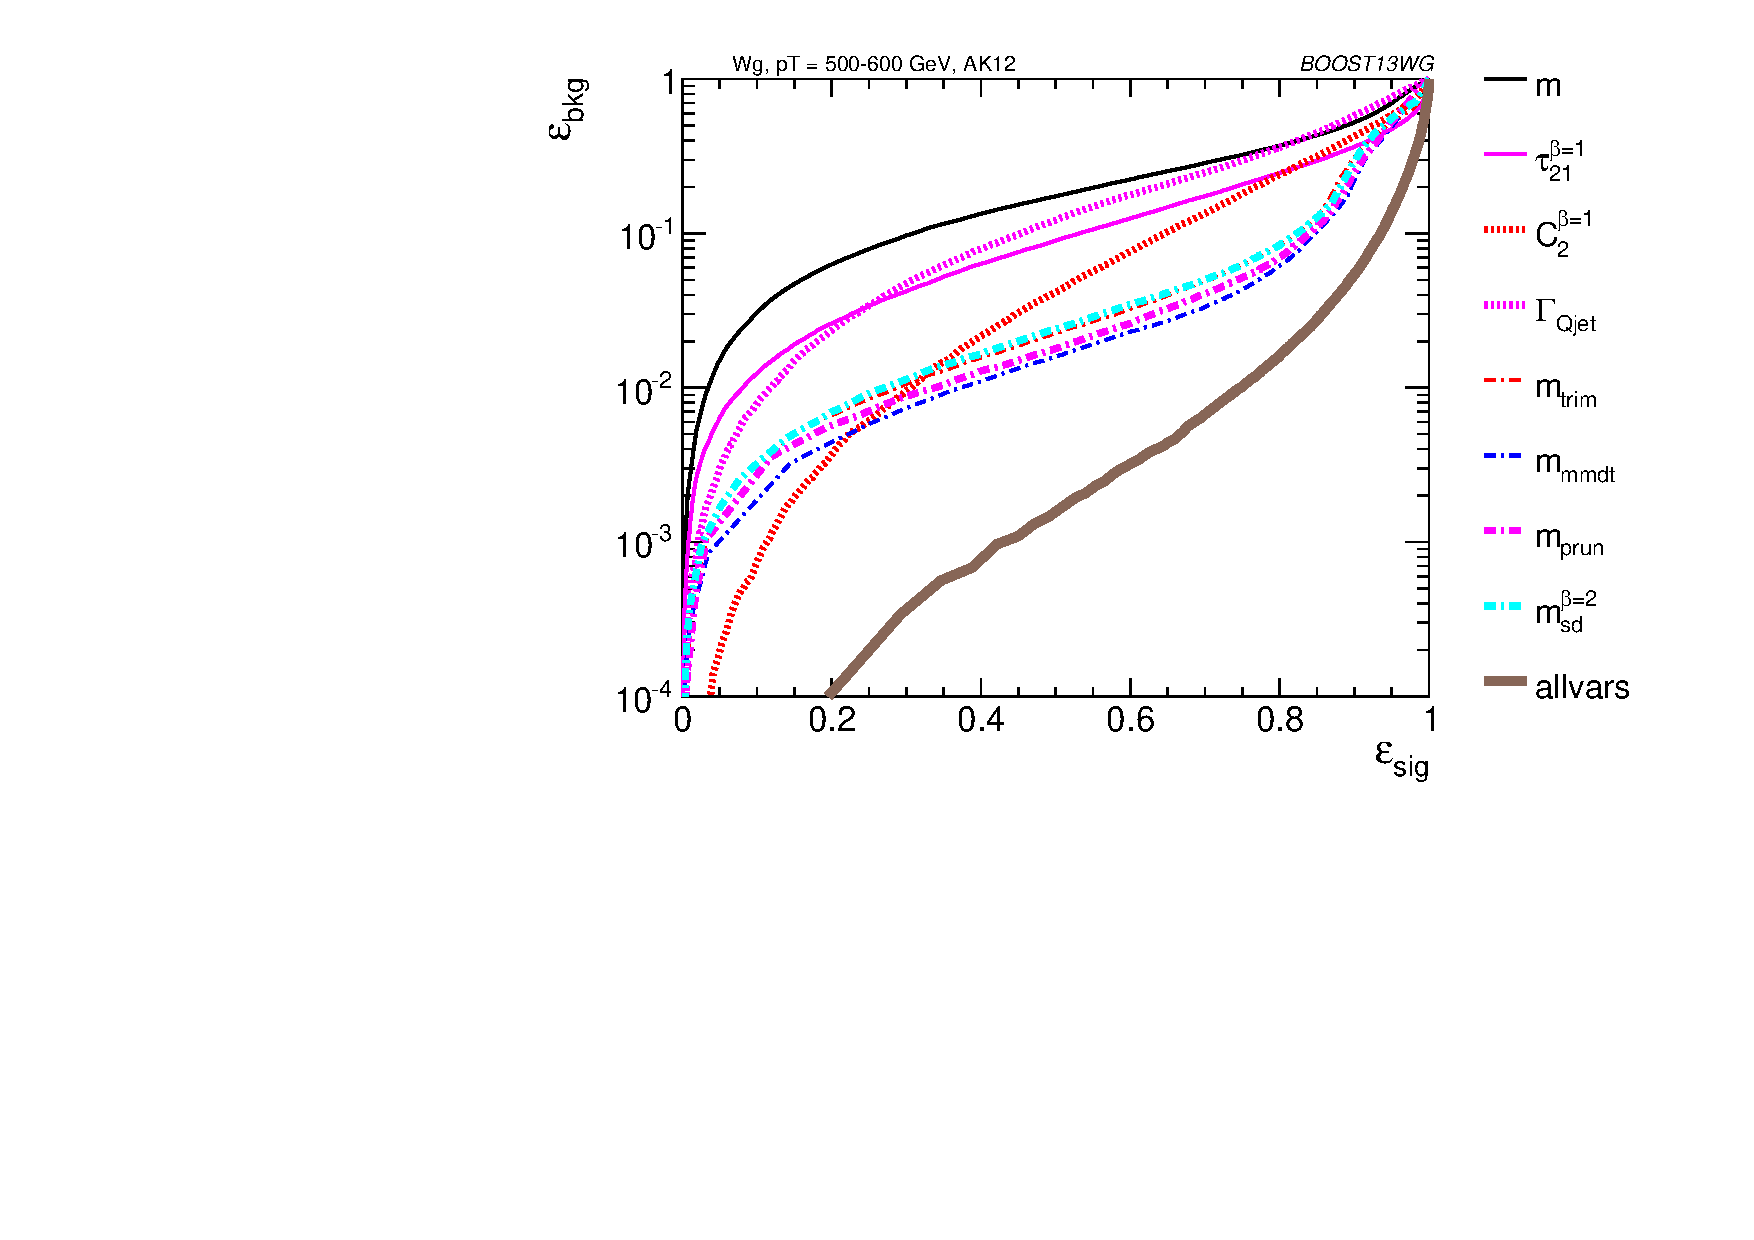
\includegraphics[width=0.48\textwidth]{./Figures/WTagging/pT500/AKtR12/Rocs_1D_single.pdf}}
\caption{ROC curves for single variables considered for $W$
tagging in the \pt = 500-600 \GeV bin using the \antikt $R=0.8$ algorithm and $R=1.2$ algorithm, along with a BDT combination of all variables (``allvars'')}
\label{fig:pt500_single}
\end{figure*}

\begin{figure*}
\centering
\subfigure[\antikt $R=0.4$, \pt = 1.0-1.1 \TeV bin]{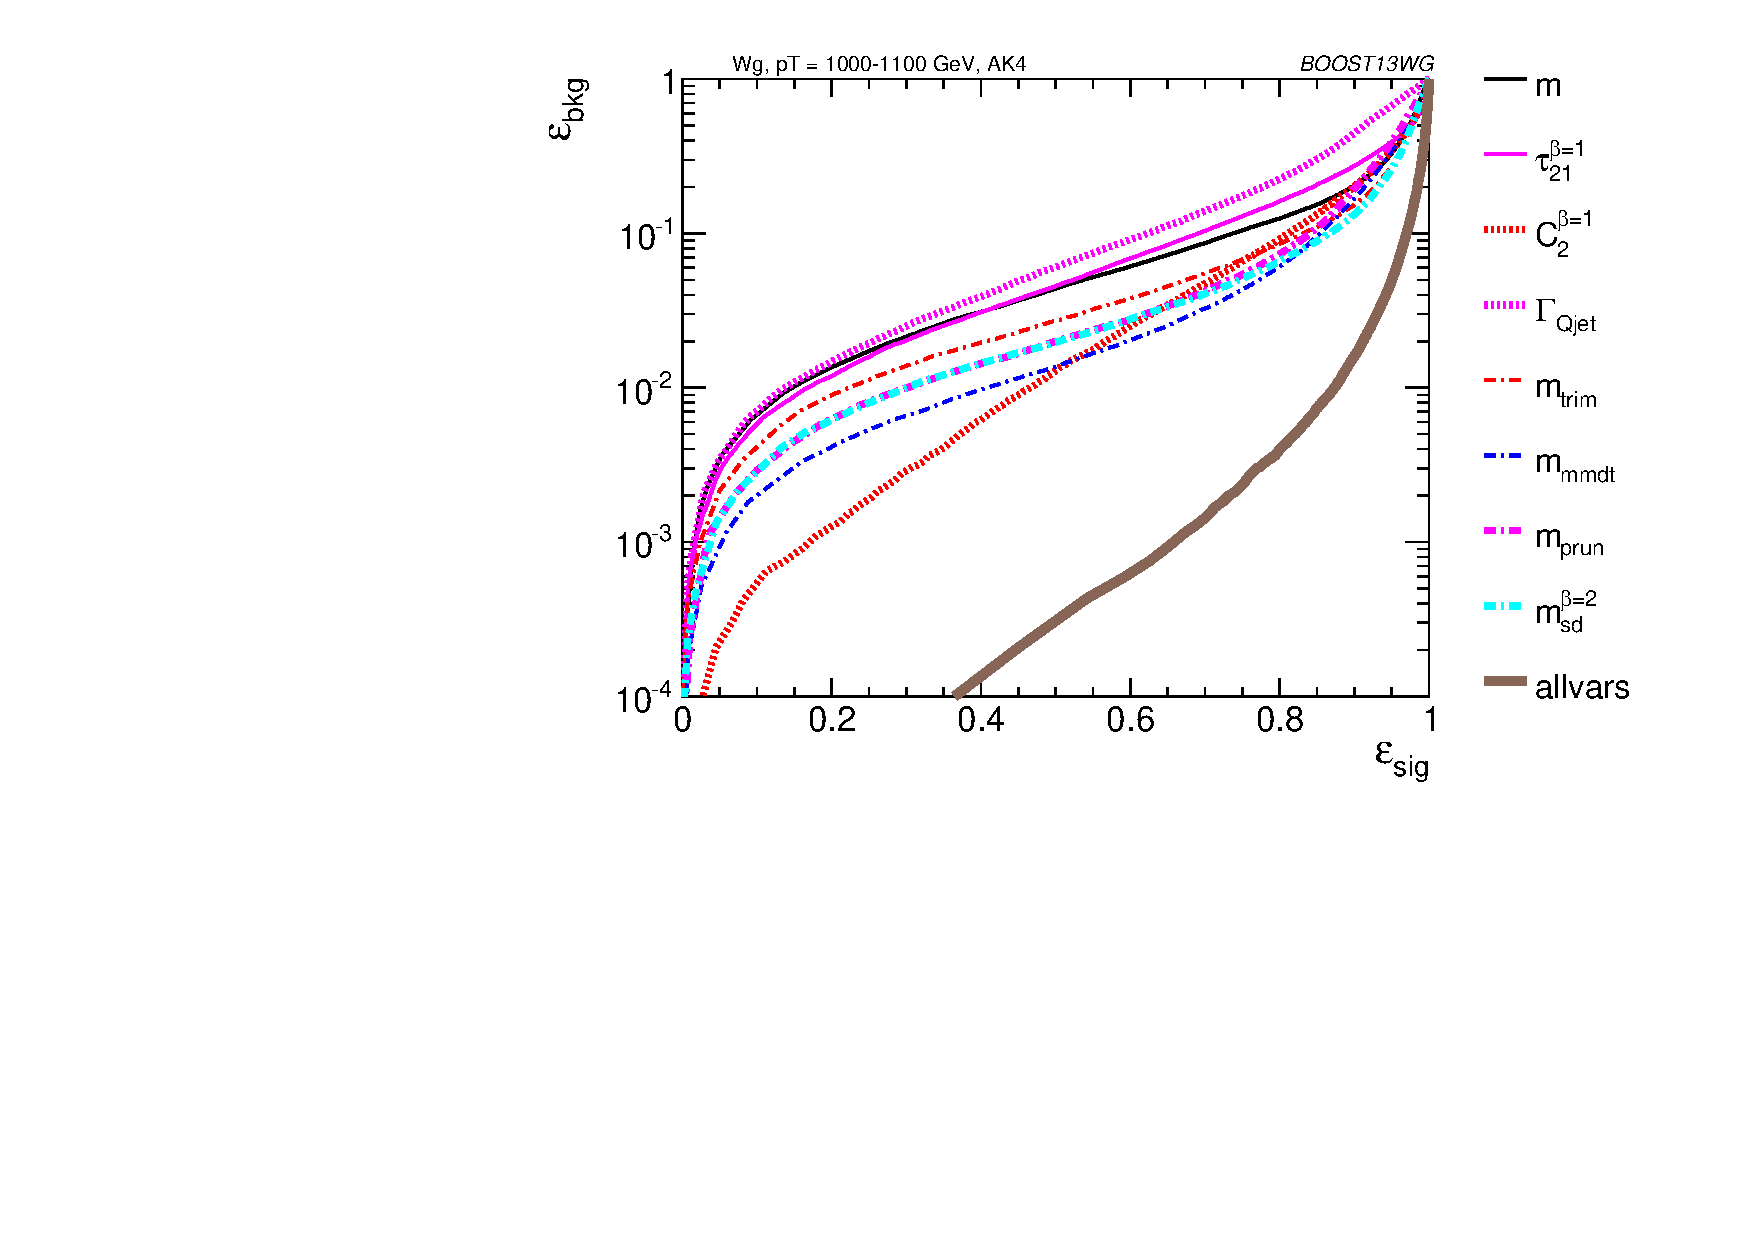
\includegraphics[width=0.48\textwidth]{./Figures/WTagging/pT1000/AKtR04/Rocs_1D_single.pdf}}
\subfigure[\antikt $R=0.8$, \pt = 1.0-1.1 \TeV bin]{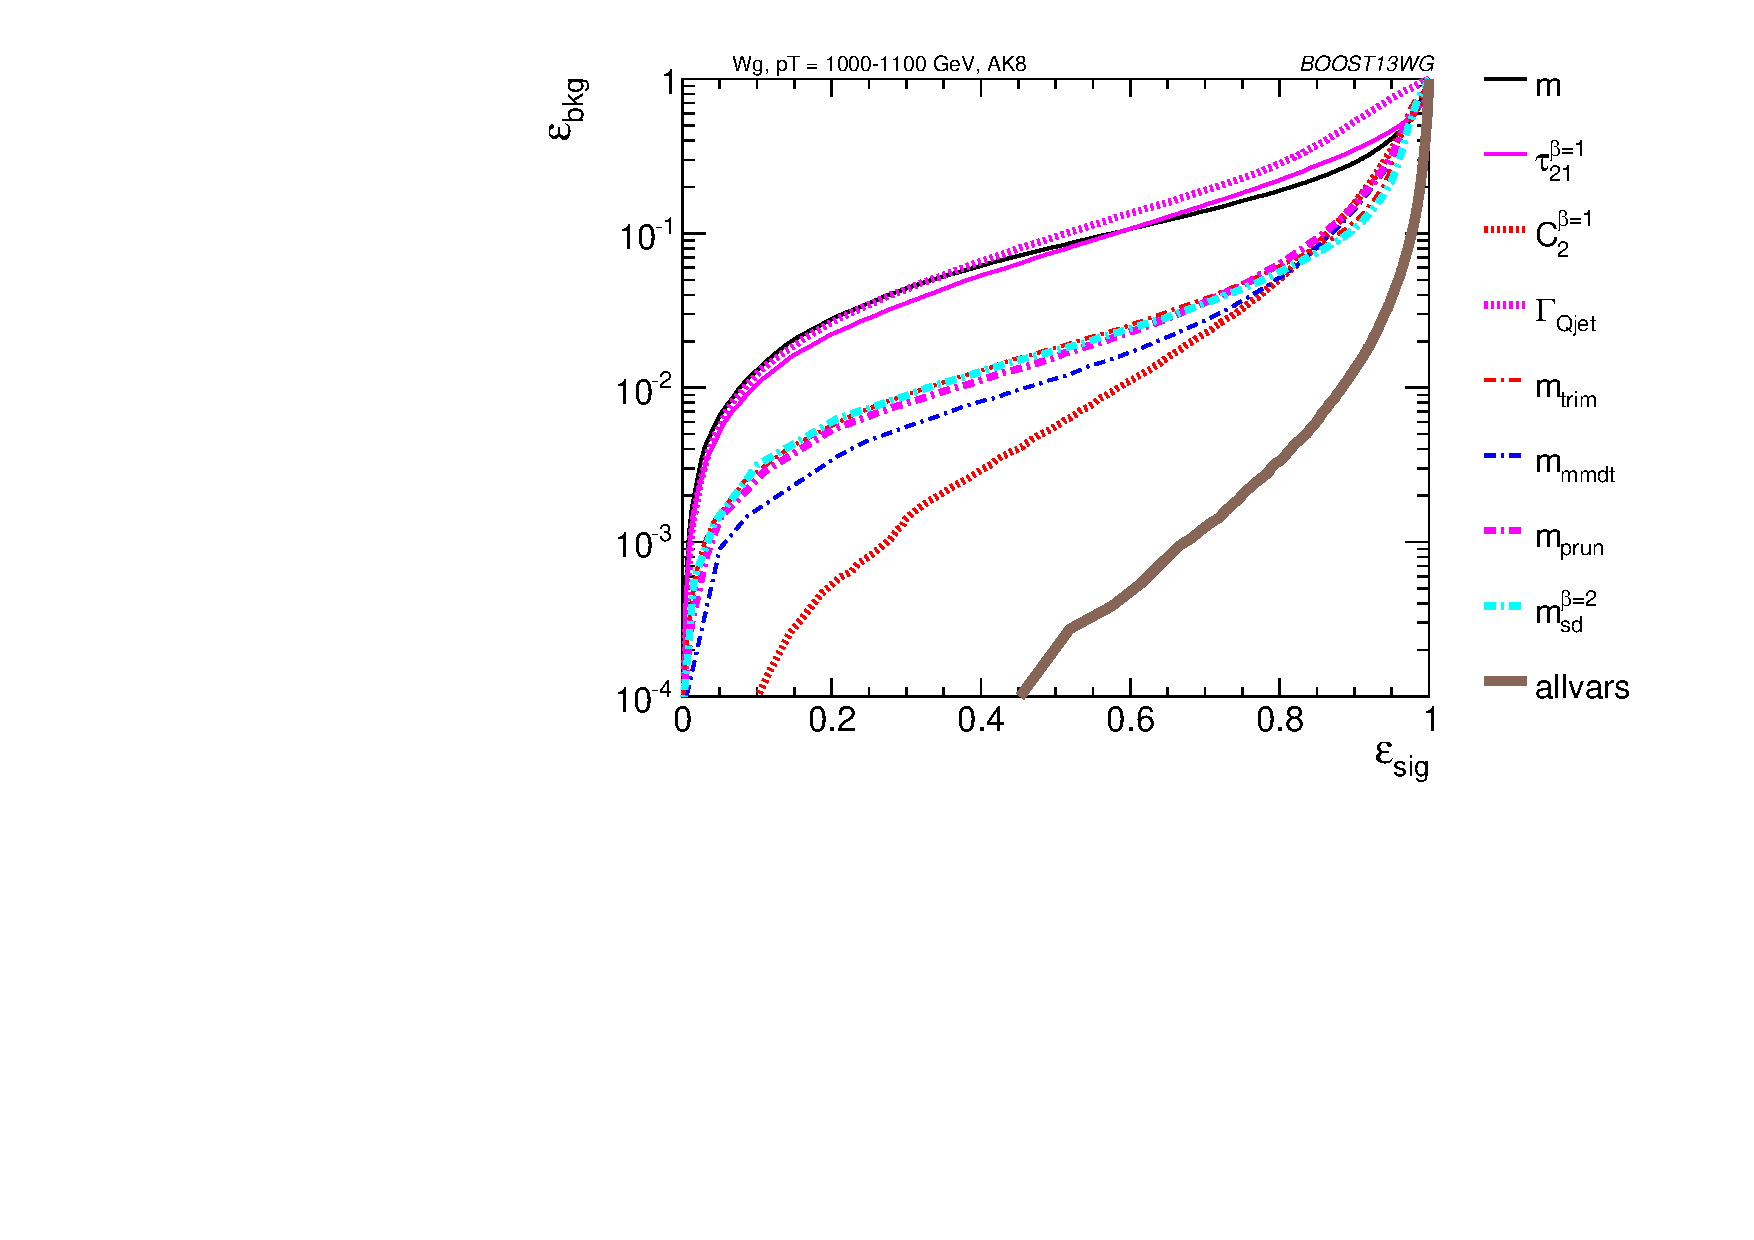
\includegraphics[width=0.48\textwidth]{./Figures/WTagging/pT1000/AKtR08/Rocs_1D_single.pdf}}\\
\subfigure[\antikt $R=1.2$, \pt = 1.0-1.1 \TeV bin]{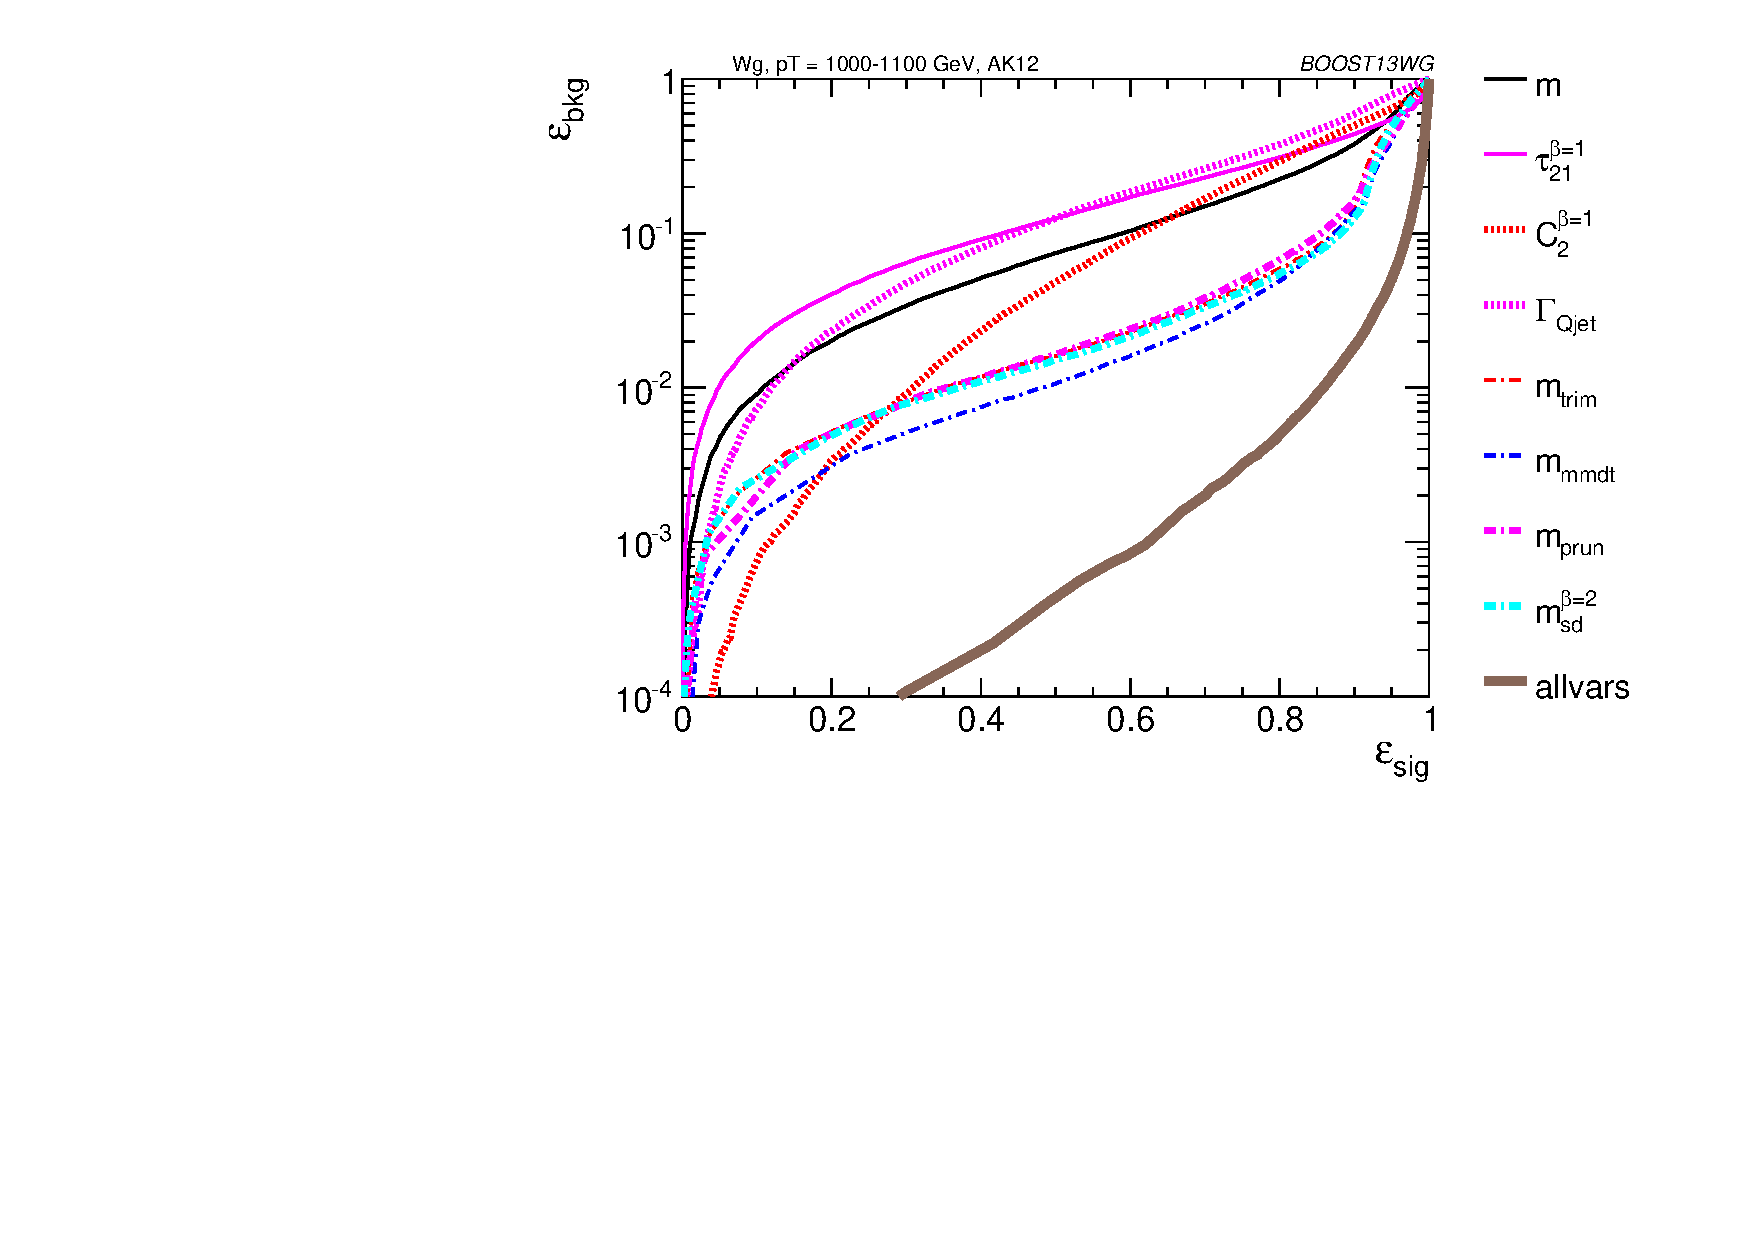
\includegraphics[width=0.48\textwidth]{./Figures/WTagging/pT1000/AKtR12/Rocs_1D_single.pdf}}
\caption{ROC curves for single variables considered for $W$
tagging in the \pt = 1.0-1.1 \TeV bin using the \antikt $R=0.4$ algorithm,
anti-\kT $R=0.8$ algorithm and $R=1.2$ algorithm, along with a BDT combination of all variables (``allvars'')}
\label{fig:pt1000_single}
\end{figure*}

%Figure~\ref{fig:pt500_single_AKt_R12} shows the single variable ROC curves in
%the \pT = 500 GeV bin for the anti-\kT R=1.2 algorithm, compared to the
%ROC curve for a BDT combination of all the variables. Comparing to
%Figure~\ref{fig:pt500_single_AKt_R08}, one can see that the
%performance of the groomed masses is quite similar. However, the
%performance of the other non-mass substructure variables is markedly
%different, and better in the R=0.8 case.
%
%\begin{figure*}
%\centering
%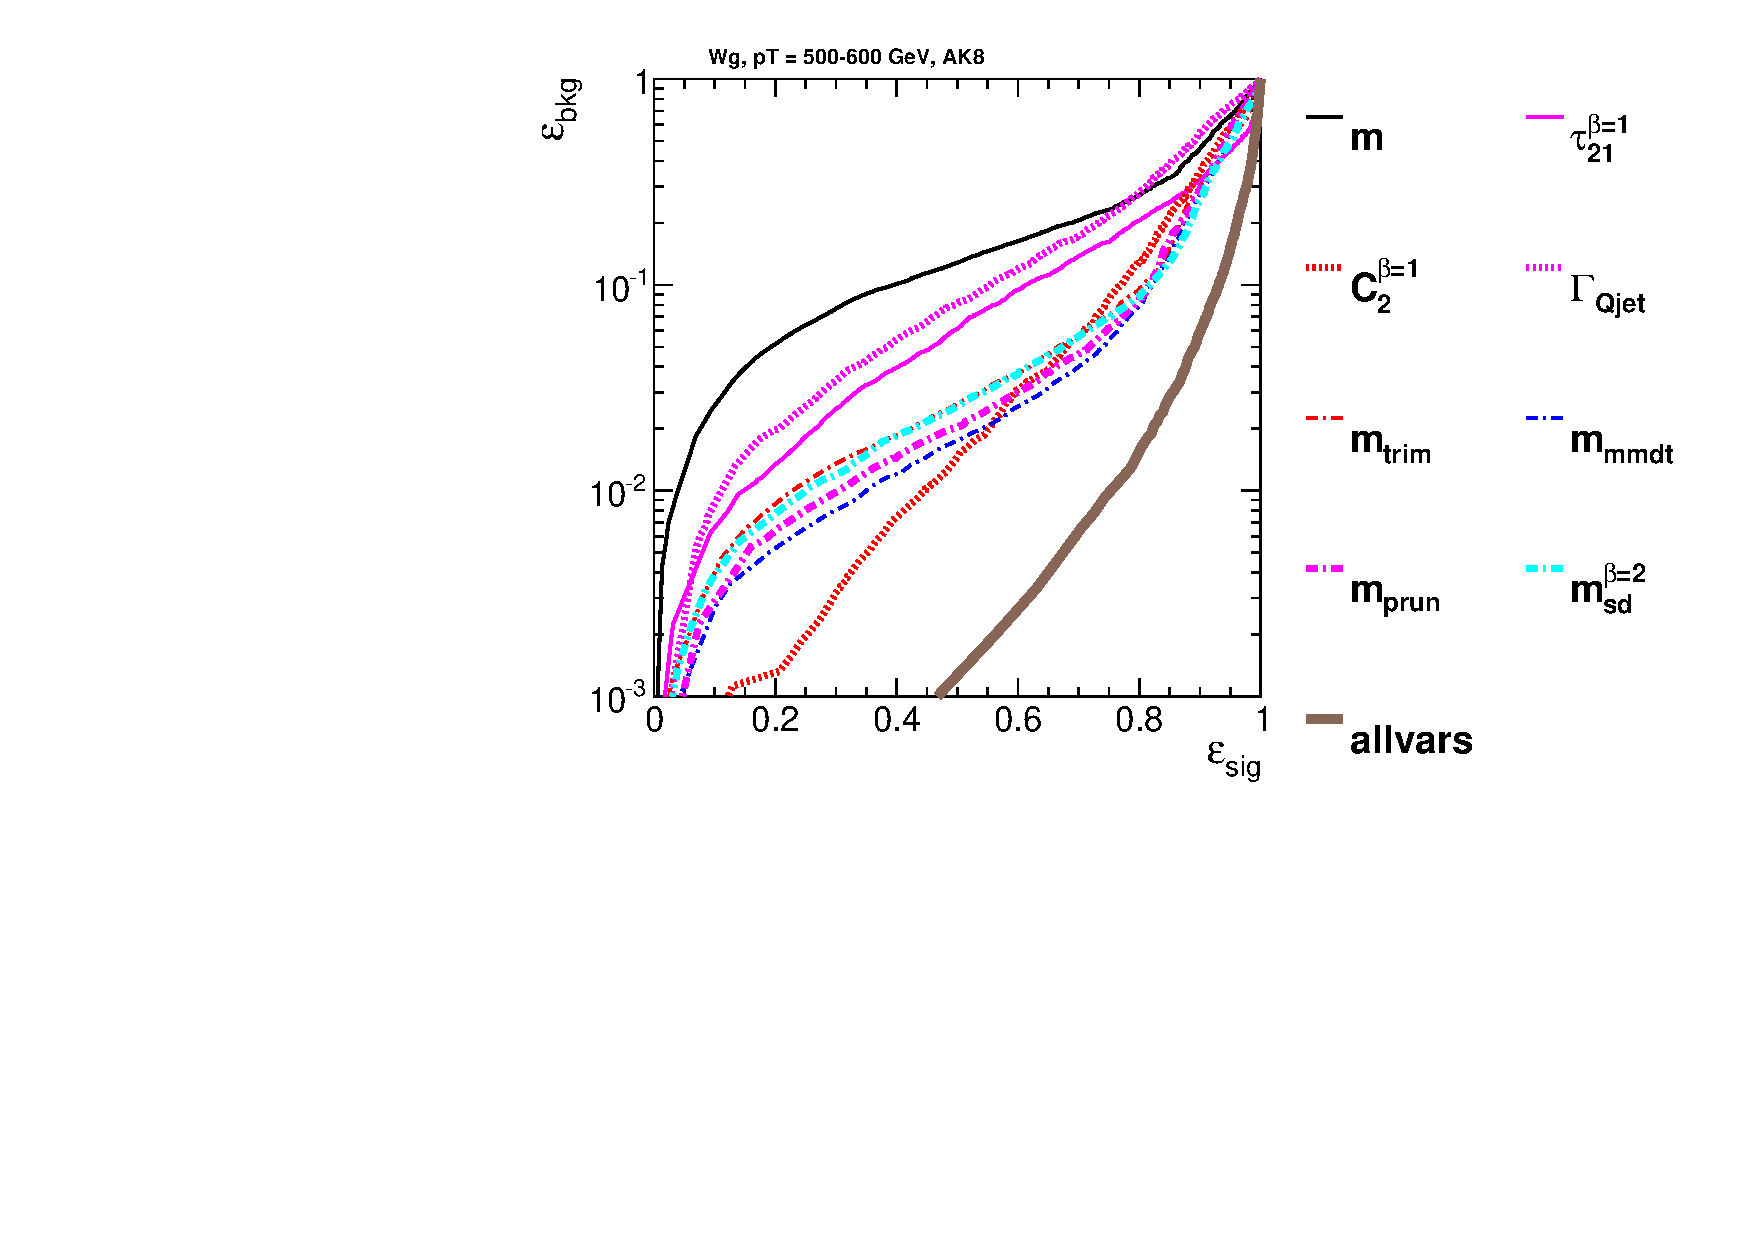
\includegraphics[width=0.8\textwidth]{./Figures/figs072514/figs071614_Wg_bin500_ak12/Rocs_1D_single.pdf}
%\caption{The ROC curve for all single variables considered for $W$
%tagging in the \pT = 500 GeV bin using the anti-\kT R=1.2 algorithm.}
%\label{fig:pt500_single_AKt_R12}
%
%\end{figure*}

 In
Figures~\ref{fig:pt300_comb2D},~\ref{fig:pt500_comb2D}
and~\ref{fig:pt1000_comb2D} the same information is shown in a format
that more readily allows for a quantitative comparison of performance
for different $R$ and \pt; matrices are presented which give the
background rejection for a signal efficiency of 70\%\footnote{Note
  that we here choose to report the rejection for a higher signal
  efficiency than the 50\% that was used in the $q/g$ tagging studies
  of Section~\ref{sec:qgtagging}, because the
rejection rates in $W$ tagging are considerably higher.} for single variable cuts, as well as two- and three-variable BDT combinations. The results are shown separately for each \pt bin and jet radius
considered.  Most relevant for our immediate discussion, the diagonal entries of these plots show the background
rejections for a single variable BDT using the labelled observable, and can thus be examined to get a
quantitative measure of the individual single variable performance,
and to study how this changes with jet radius and momenta. The off-diagonal
entries give the performance when two variables (shown on the x-axis and on the y-axis, respectively) are combined in
a BDT. The
final column of these plots shows the background rejection
performance for three-variable BDT combinations of $m_{sd}^{\beta=2} +
C_2^{\beta=1} + X$. These results will be discussed later in Section~\ref{sec:Wtagallvars}. 

\begin{figure*}
\centering
\subfigure[\antikt $R=0.8$, \pt = 300-400 \GeV bin]{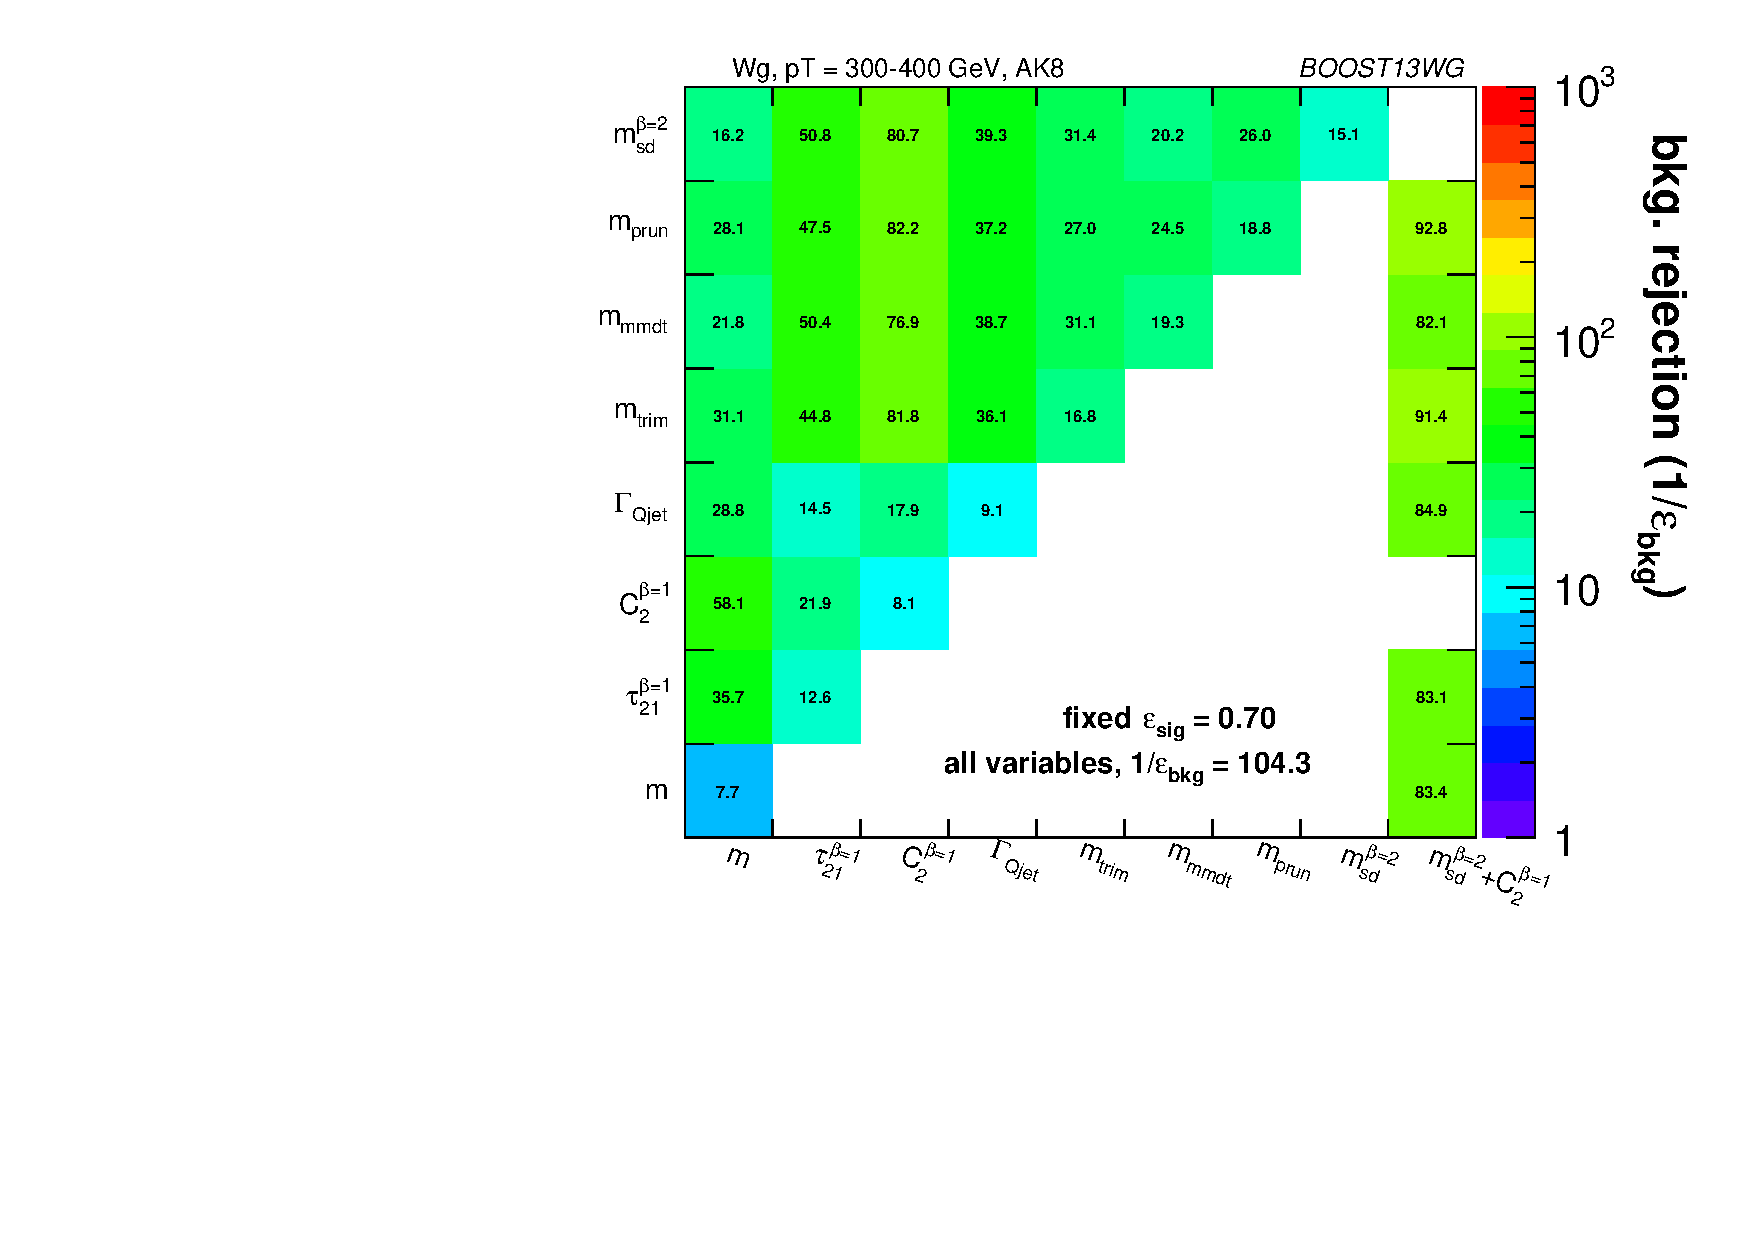
\includegraphics[width=0.48\textwidth]{./Figures/WTagging/pT300/AKtR08/effBkg2D.pdf}\label{fig:pt300_comb2D_08}}
\subfigure[\antikt $R=1.2$, \pt = 300-400 \GeV bin]{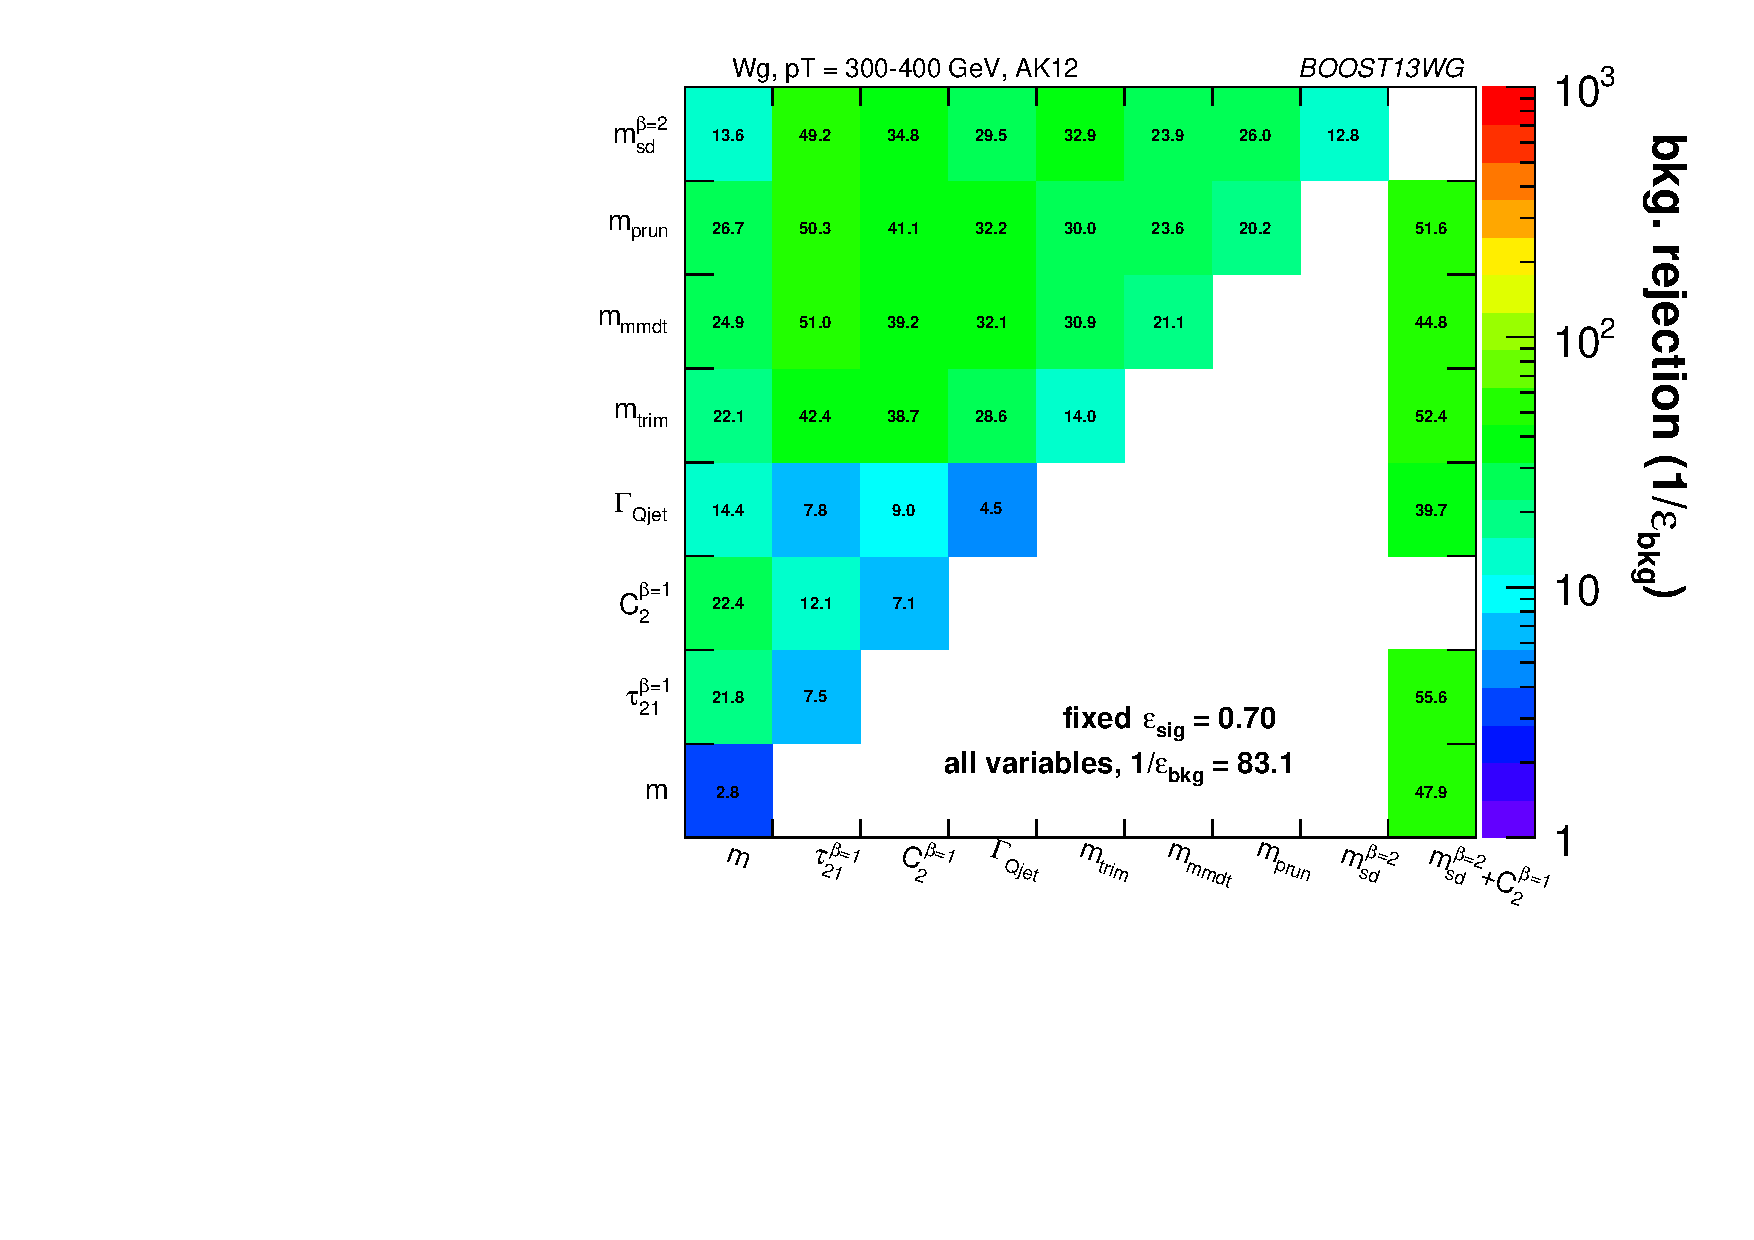
\includegraphics[width=0.48\textwidth]{./Figures/WTagging/pT300/AKtR12/effBkg2D.pdf}\label{fig:pt300_comb2D_12}}
\caption{
The background rejection
for a fixed signal efficiency (70\%) of each BDT combination of
each pair of variables considered, in the \pt = 300-400 \GeV bin using the anti-\kT $R=0.8$
algorithm and $R=1.2$ algorithm. Also shown is the background
rejection for three-variable combinations involving $m_{sd}^{\beta=2} +
C_2^{\beta=1}$, and for a BDT combination of all of the variables considered.
}
\label{fig:pt300_comb2D}
\end{figure*}


\begin{figure*}
\centering
\subfigure[\antikt $R=0.8$, \pt = 500-600 \GeV bin]{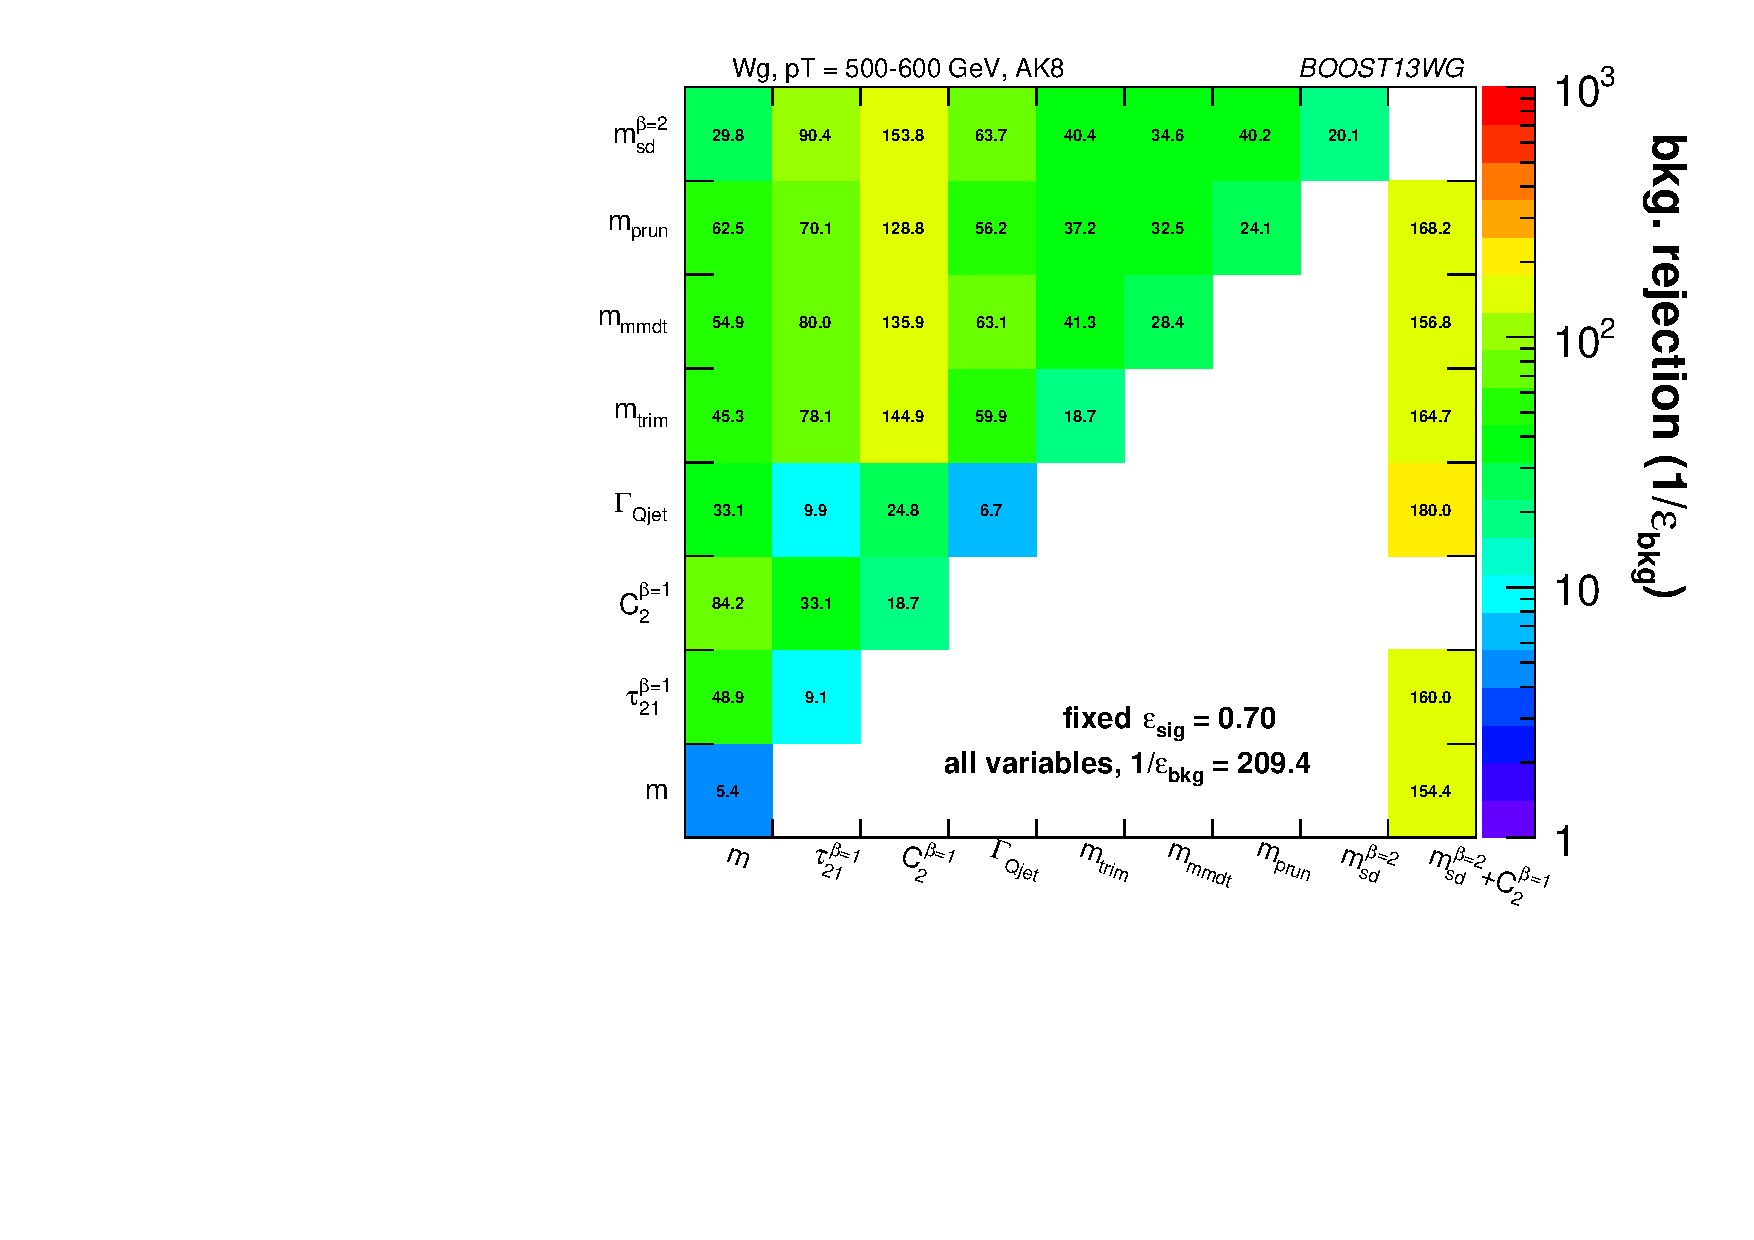
\includegraphics[width=0.48\textwidth]{./Figures/WTagging/pT500/AKtR08/effBkg2D.pdf}\label{fig:pt500_comb2D_08}}
\subfigure[\antikt $R=1.2$, \pt = 500-600 \GeV bin]{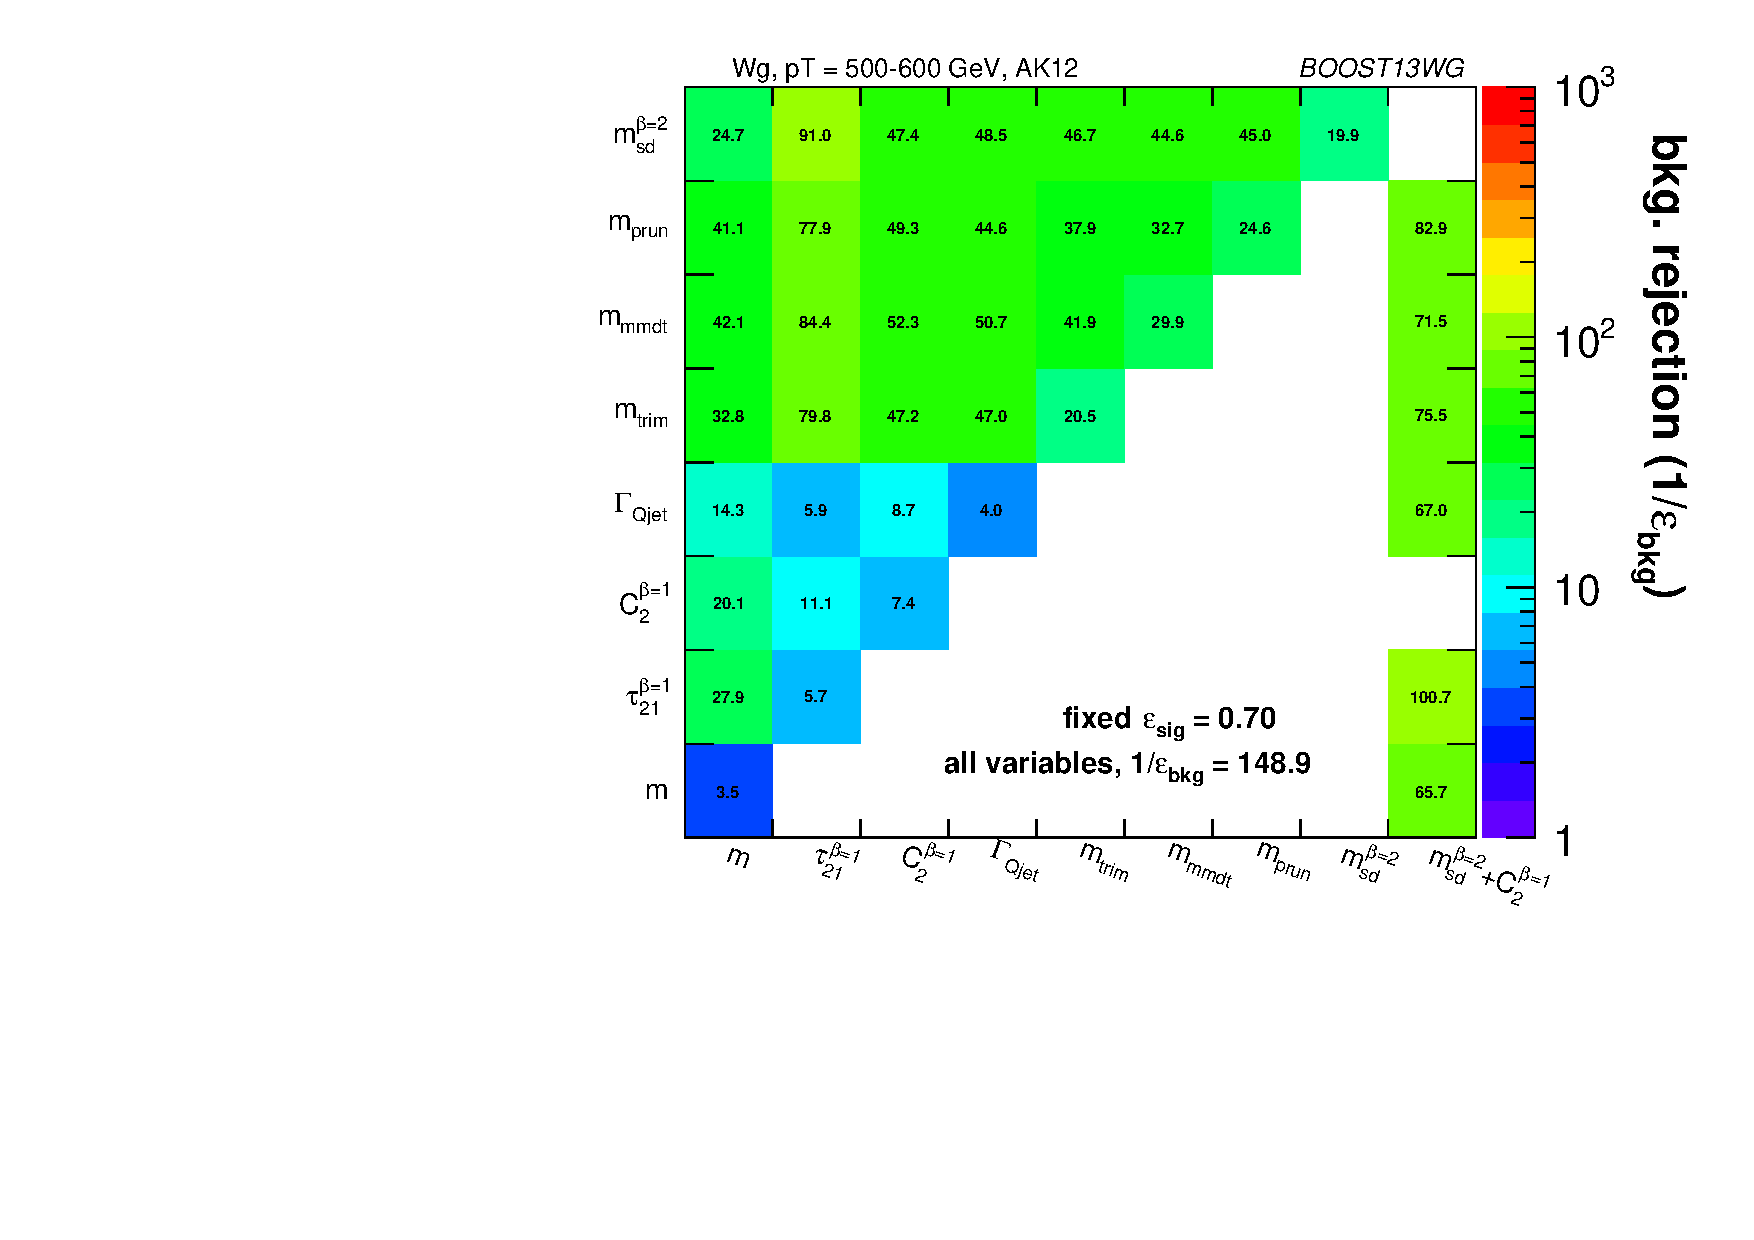
\includegraphics[width=0.48\textwidth]{./Figures/WTagging/pT500/AKtR12/effBkg2D.pdf}\label{fig:pt500_comb2D_12}}
\caption{The background rejection
for a fixed signal efficiency (70\%) of each BDT combination of
each pair of variables considered, in the \pt = 500-600 \GeV bin using the \antikt $R=0.8$
algorithm and $R=1.2$ algorithm. Also shown is the background
rejection for three-variable combinations involving $m_{sd}^{\beta=2} +
C_2^{\beta=1}$, and for a BDT combination of all of the variables considered.}
\label{fig:pt500_comb2D}
\end{figure*}

\begin{figure*}
\centering
\subfigure[\antikt $R=0.4$, \pt = 1.0-1.1 \TeV bin]{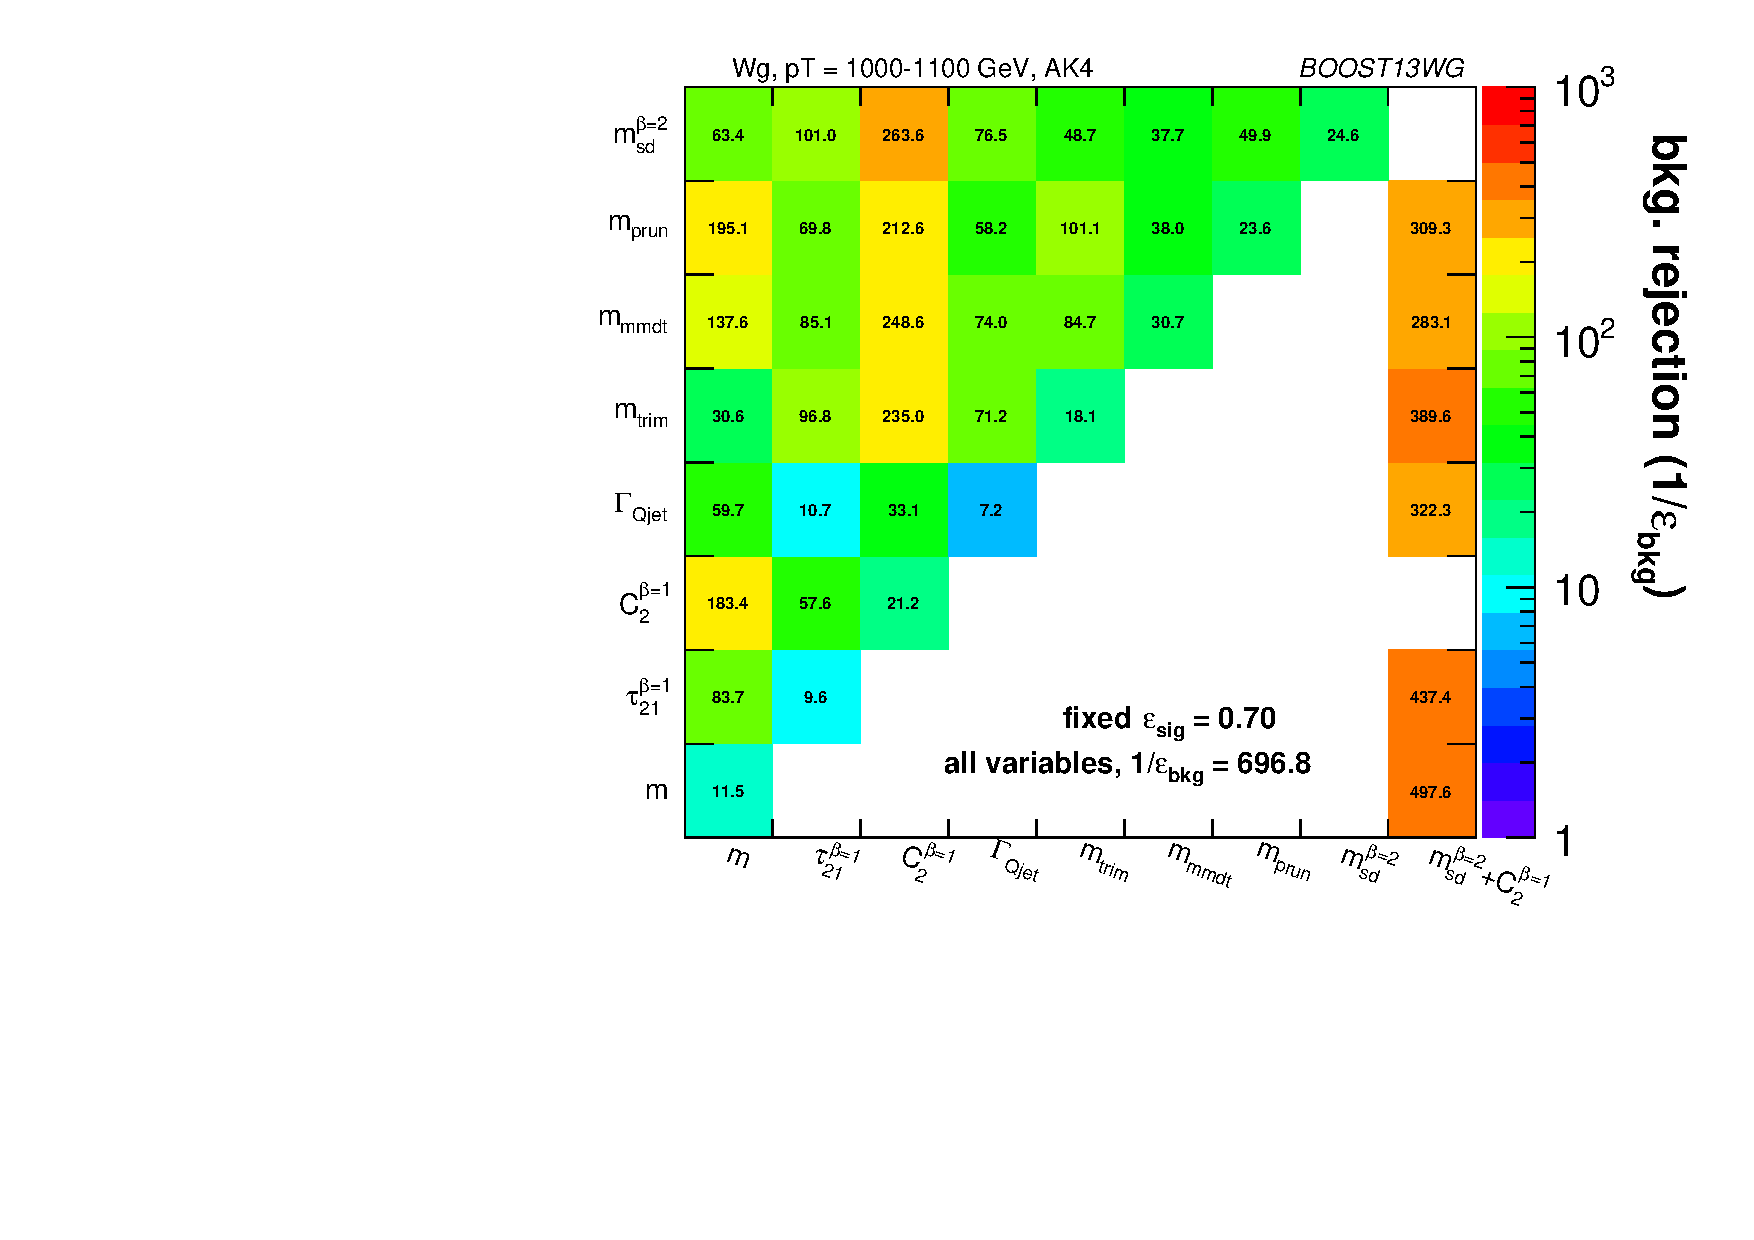
\includegraphics[width=0.48\textwidth]{./Figures/WTagging/pT1000/AKtR04/effBkg2D.pdf}\label{fig:pt1000_comb2D_04}}
\subfigure[\antikt $R=0.8$, \pt = 1.0-1.1 \TeV bin]{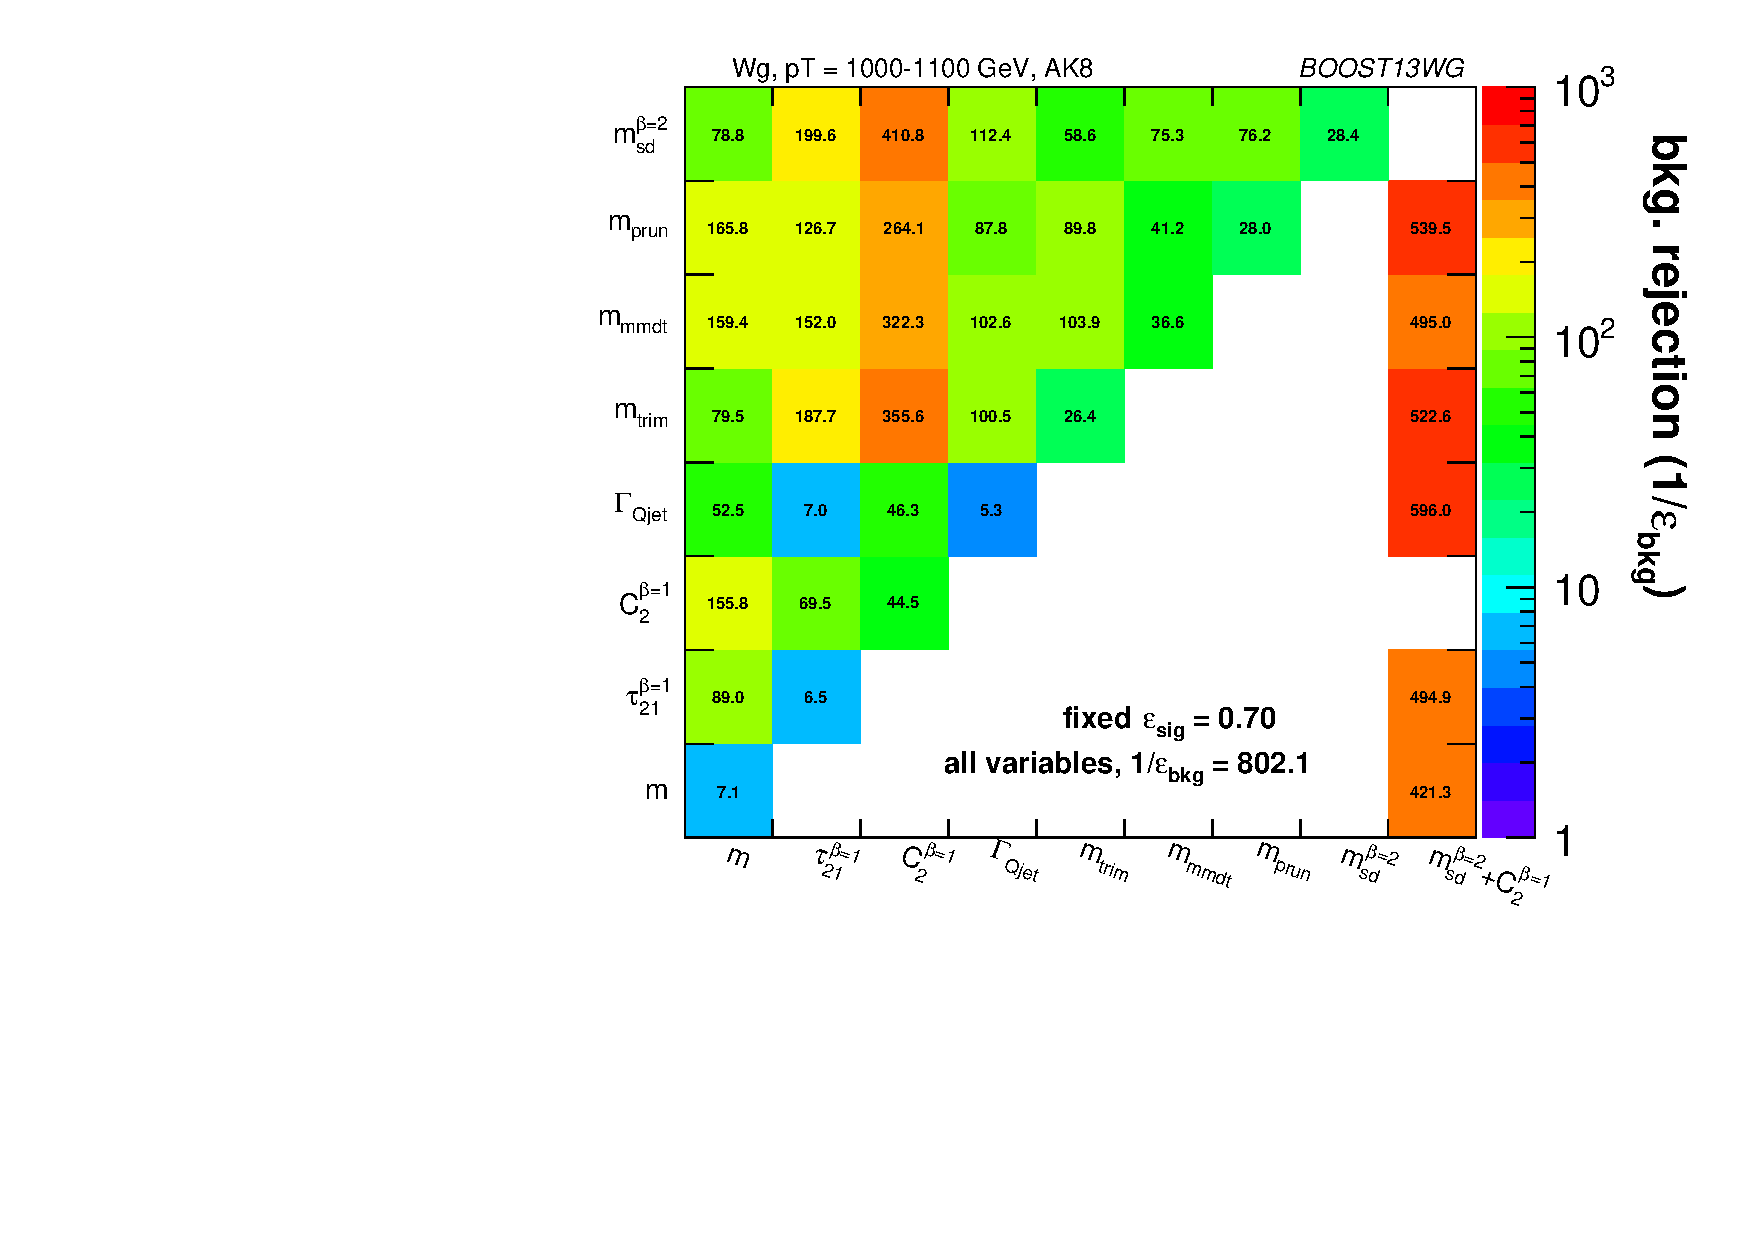
\includegraphics[width=0.48\textwidth]{./Figures/WTagging/pT1000/AKtR08/effBkg2D.pdf}\label{fig:pt1000_comb2D_08}}\\
\subfigure[\antikt $R=1.2$, \pt = 1.0-1.1 \TeV bin]{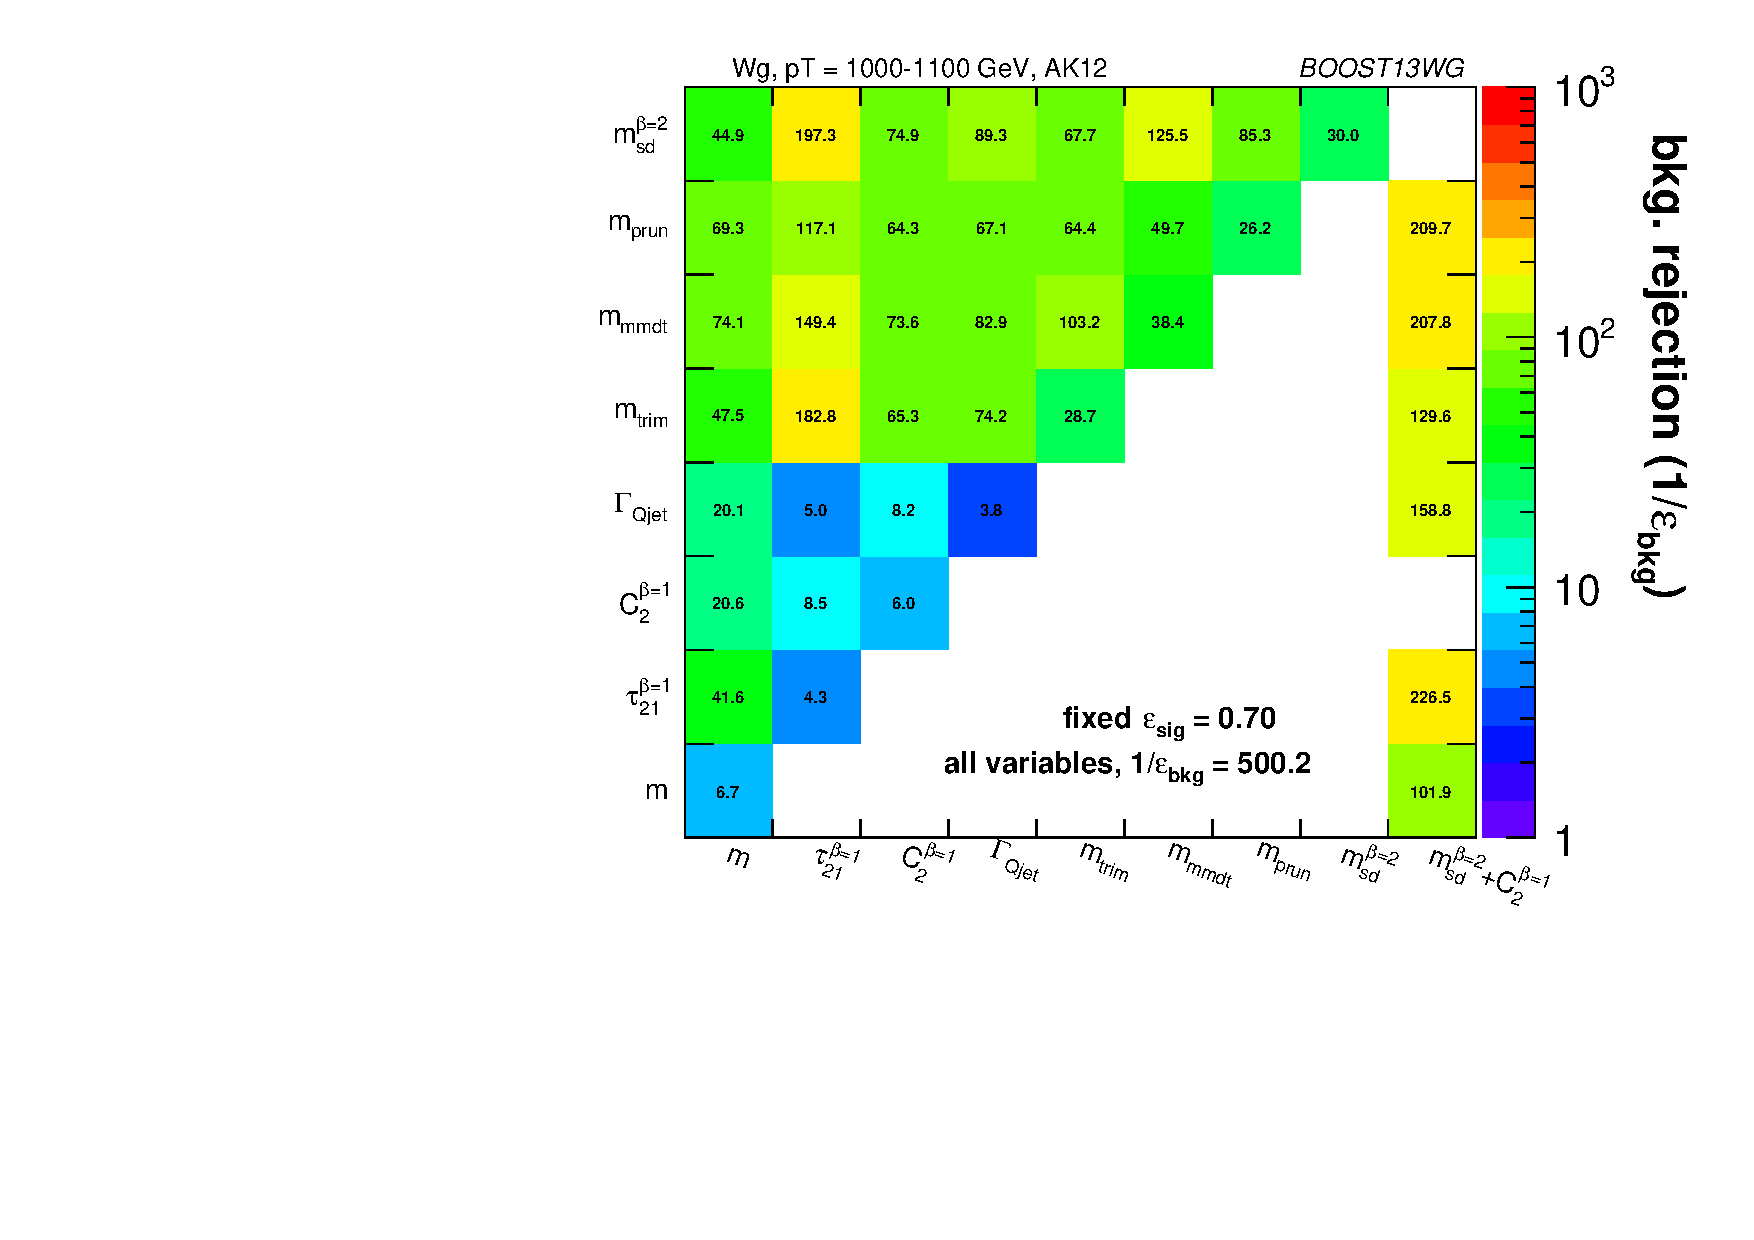
\includegraphics[width=0.48\textwidth]{./Figures/WTagging/pT1000/AKtR12/effBkg2D.pdf}\label{fig:pt1000_comb2D_12}}
\caption{The background rejection
for a fixed signal efficiency (70\%) of each BDT combination of
each pair of variables considered, in the \pt = 1.0-1.1 \TeV bin using
the anti-\kT $R=0.4$, $R=0.8$ and $R=1.2$ algorithm. Also shown is the background
rejection for three-variable combinations involving $m_{sd}^{\beta=2} +
C_2^{\beta=1}$, and for a BDT combination of all of the variables considered.}
\label{fig:pt1000_comb2D}
\end{figure*}



In general, the most performant single variables are
the groomed masses. However, in certain kinematic bins and for certain
jet radii, $C_2^{\beta=1}$ has a background rejection that is
comparable to or better than the groomed masses. 

%By comparing Figures~\ref{fig:pt300_comb2D_08}
%and~\ref{fig:pt300_comb2D_12}, Figures 
We first examine the variation of performance with jet \pt. By comparing
Figures~\ref{fig:pt300_comb2D_08},~\ref{fig:pt500_comb2D_08}
and~\ref{fig:pt1000_comb2D_08}, we can see how the background
rejection performance varies with increased momenta whilst keeping the jet
radius fixed to $R=0.8$. Similarly, by comparing Figures~\ref{fig:pt300_comb2D_12},~\ref{fig:pt500_comb2D_12}
and~\ref{fig:pt1000_comb2D_12} we can see how performance evolves with
\pt for $R=1.2$. For both $R=0.8$ and $R=1.2$ the background rejection power of
the groomed masses increases with increasing \pt, with a factor 1.5-2.5 increase in rejection in going from the 300-400 GeV to
1.0-1.1 TeV bins. In Figure~\ref{fig:ptdepend_groomedmass} we show the
\msd and \mprun groomed masses for signal and background in the \pt = 300-400 and \pt = 1.0-1.1 \TeV bins for $R=1.2$ jets. Two effects result in the improved
performance of the groomed mass at high \pt. Firstly, as is evident
from the figure, the resolution of the signal peak after grooming
improves, because the groomer finds it easier to pick out the hard
signal component of the jet against the softer components of the
underlying event when the signal is boosted. Secondly, it follows
from Figure~\ref{fig:qg_prmasses_log} and the discussion in Section~\ref{sec:qg_mass}
that, for increasing \pt, the perturbative shoulder of the gluon
distribution decreases in size, and
thus there is a slight decrease (or at least no increase) of the background contamination in the
signal mass region (m/$p_{T}$/R $\sim$ 0.5). 
%as the \pT increases, more of the gluon
%background in the W mass window comes from jets building up their
%masses from radiation that can be understood in the eikonal limits and
%not from hard splittings. This is precisely the radiation grooming
%methods are designed to remove, and so their performance increases with \pT.  

\begin{figure*}
\centering
\subfigure[\antikt $R=1.2$, \pt = 300-400 \GeV bin]{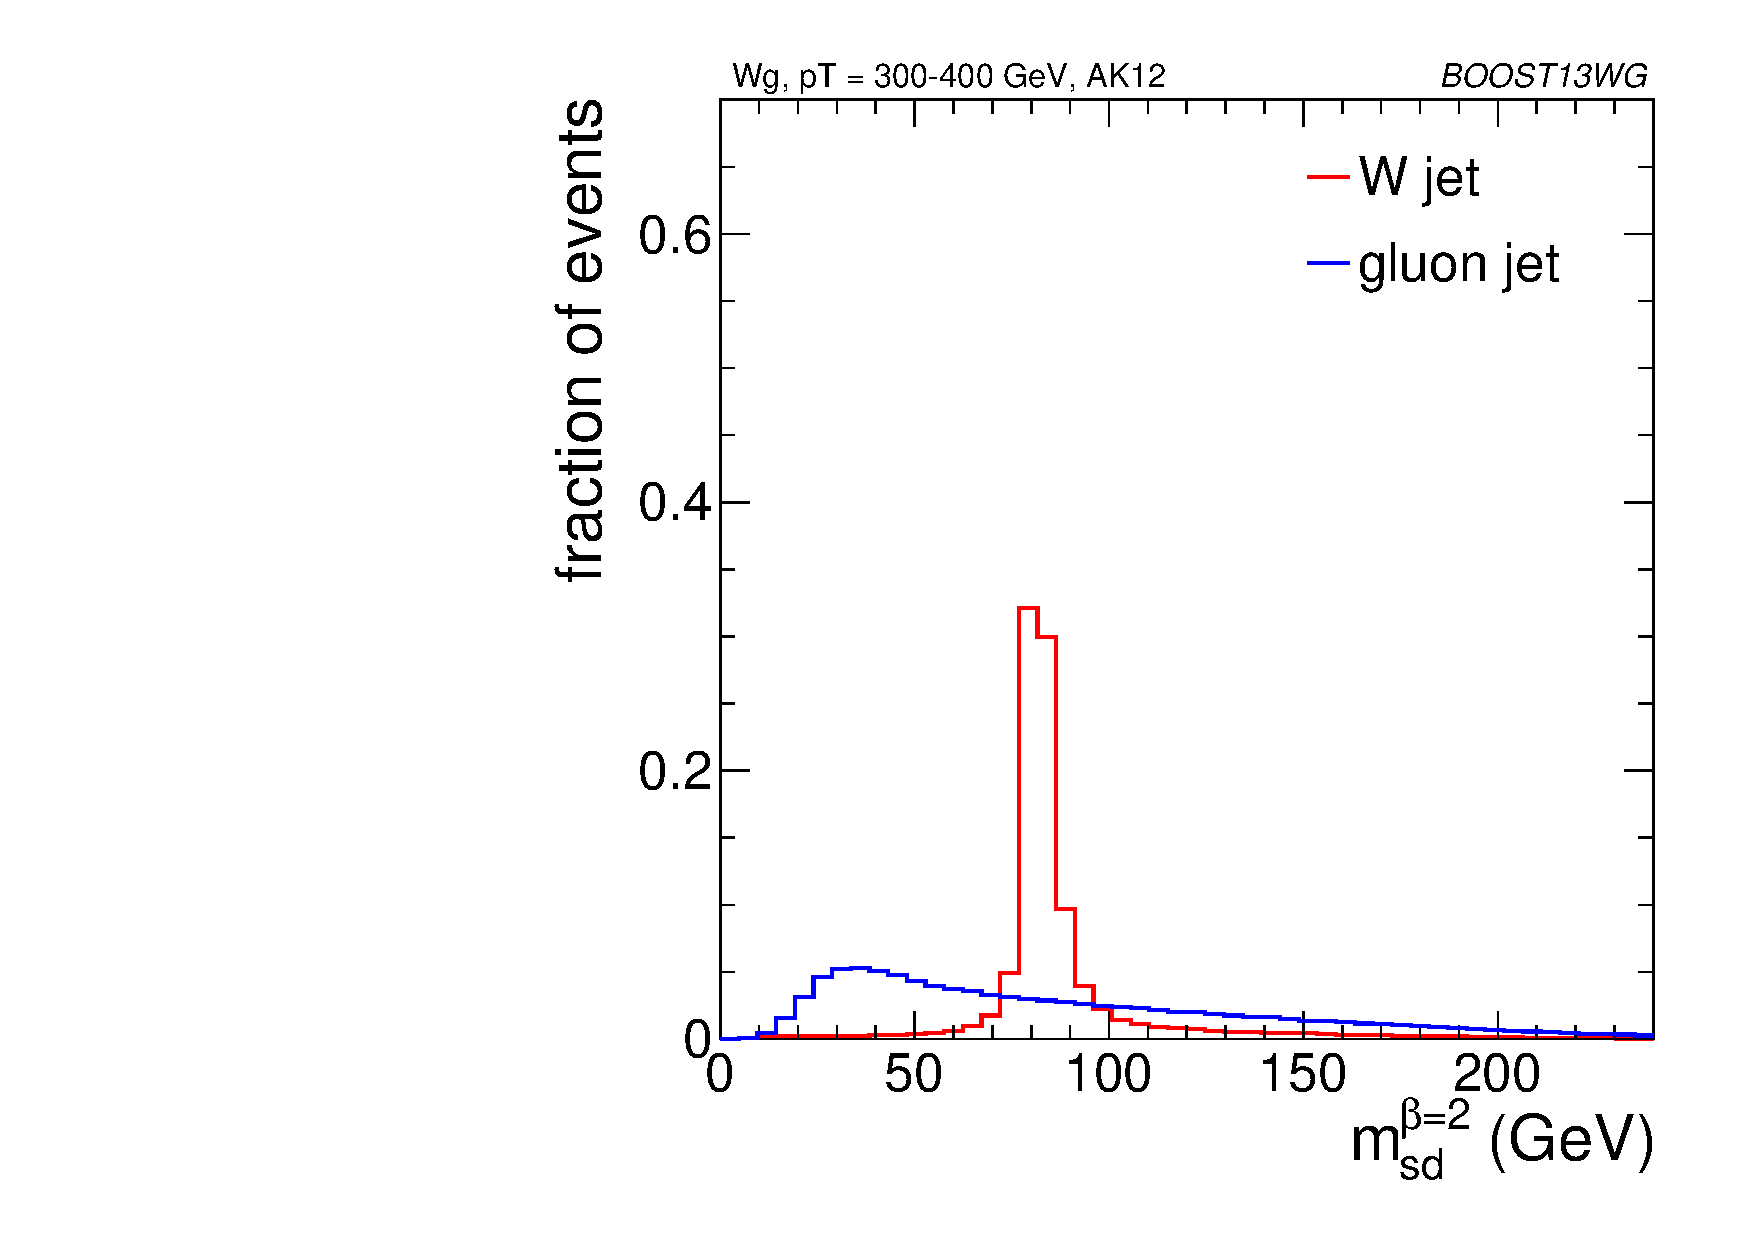
\includegraphics[width=0.4\textwidth]{./Figures/WTagging/pT300/AKtR12/h_mass_sdb2.pdf}}
\subfigure[\antikt $R=1.2$, \pt = 1.0-1.1 \TeV bin]{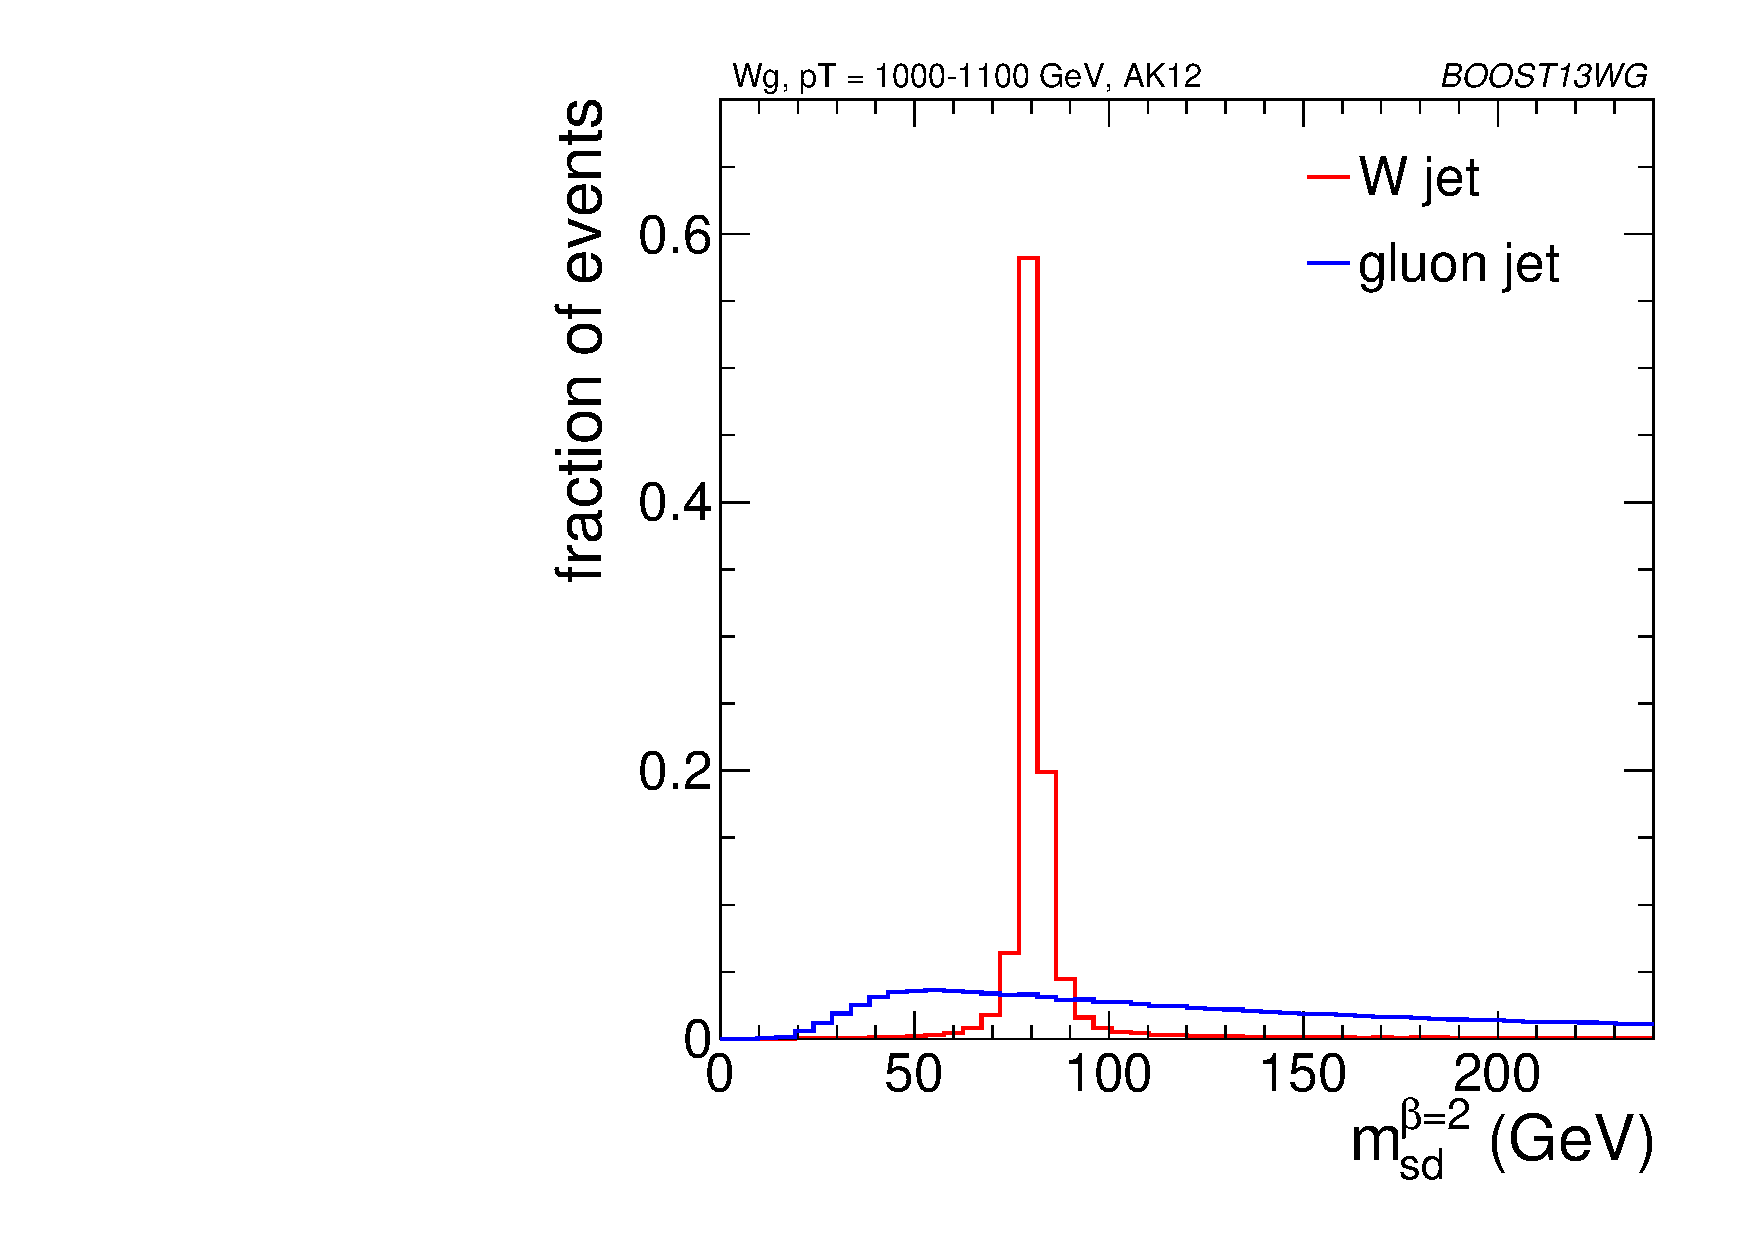
\includegraphics[width=0.4\textwidth]{./Figures/WTagging/pT1000/AKtR12/h_mass_sdb2.pdf}}
\subfigure[\antikt $R=1.2$, \pt = 300-400 \GeV bin]{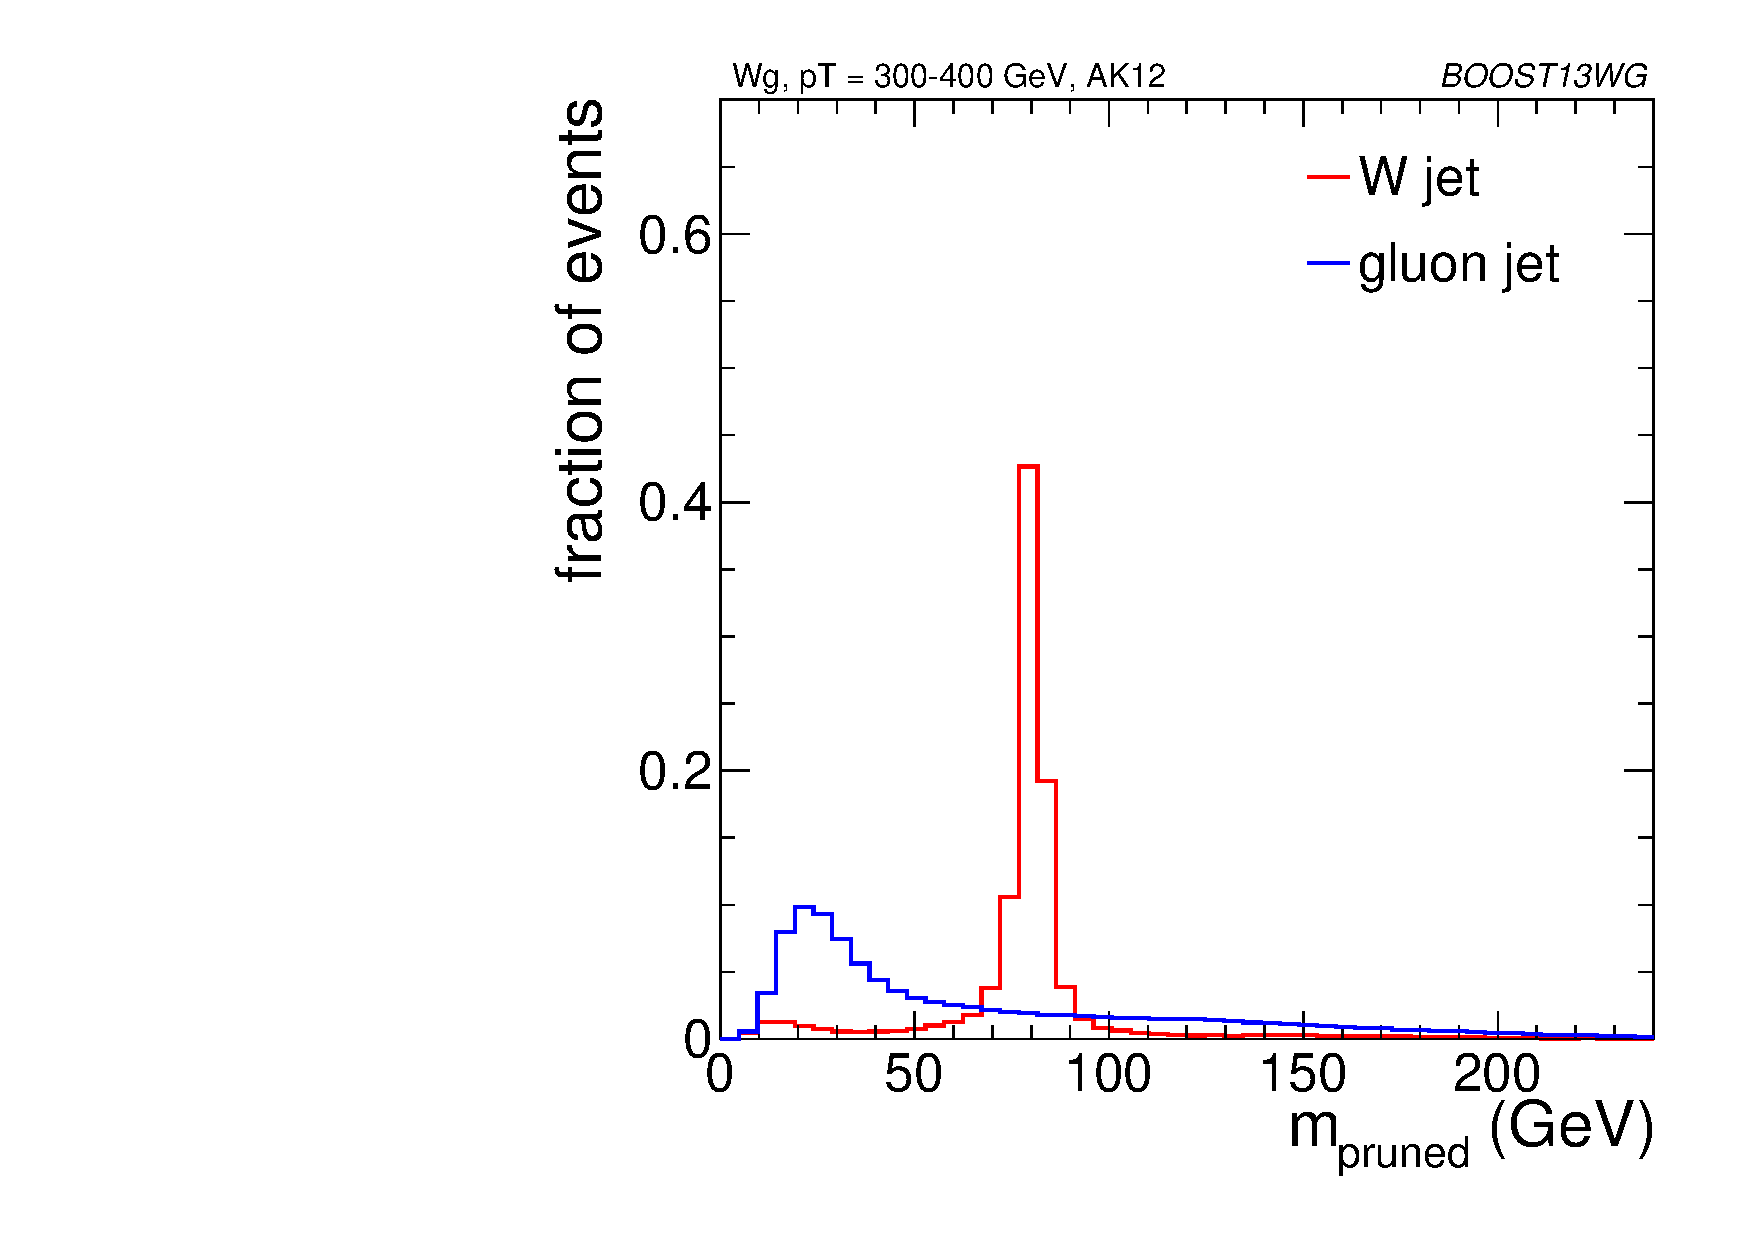
\includegraphics[width=0.4\textwidth]{./Figures/WTagging/pT300/AKtR12/h_mass_prun.pdf}}
\subfigure[\antikt $R=1.2$, \pt = 1.0-1.1 \TeV bin]{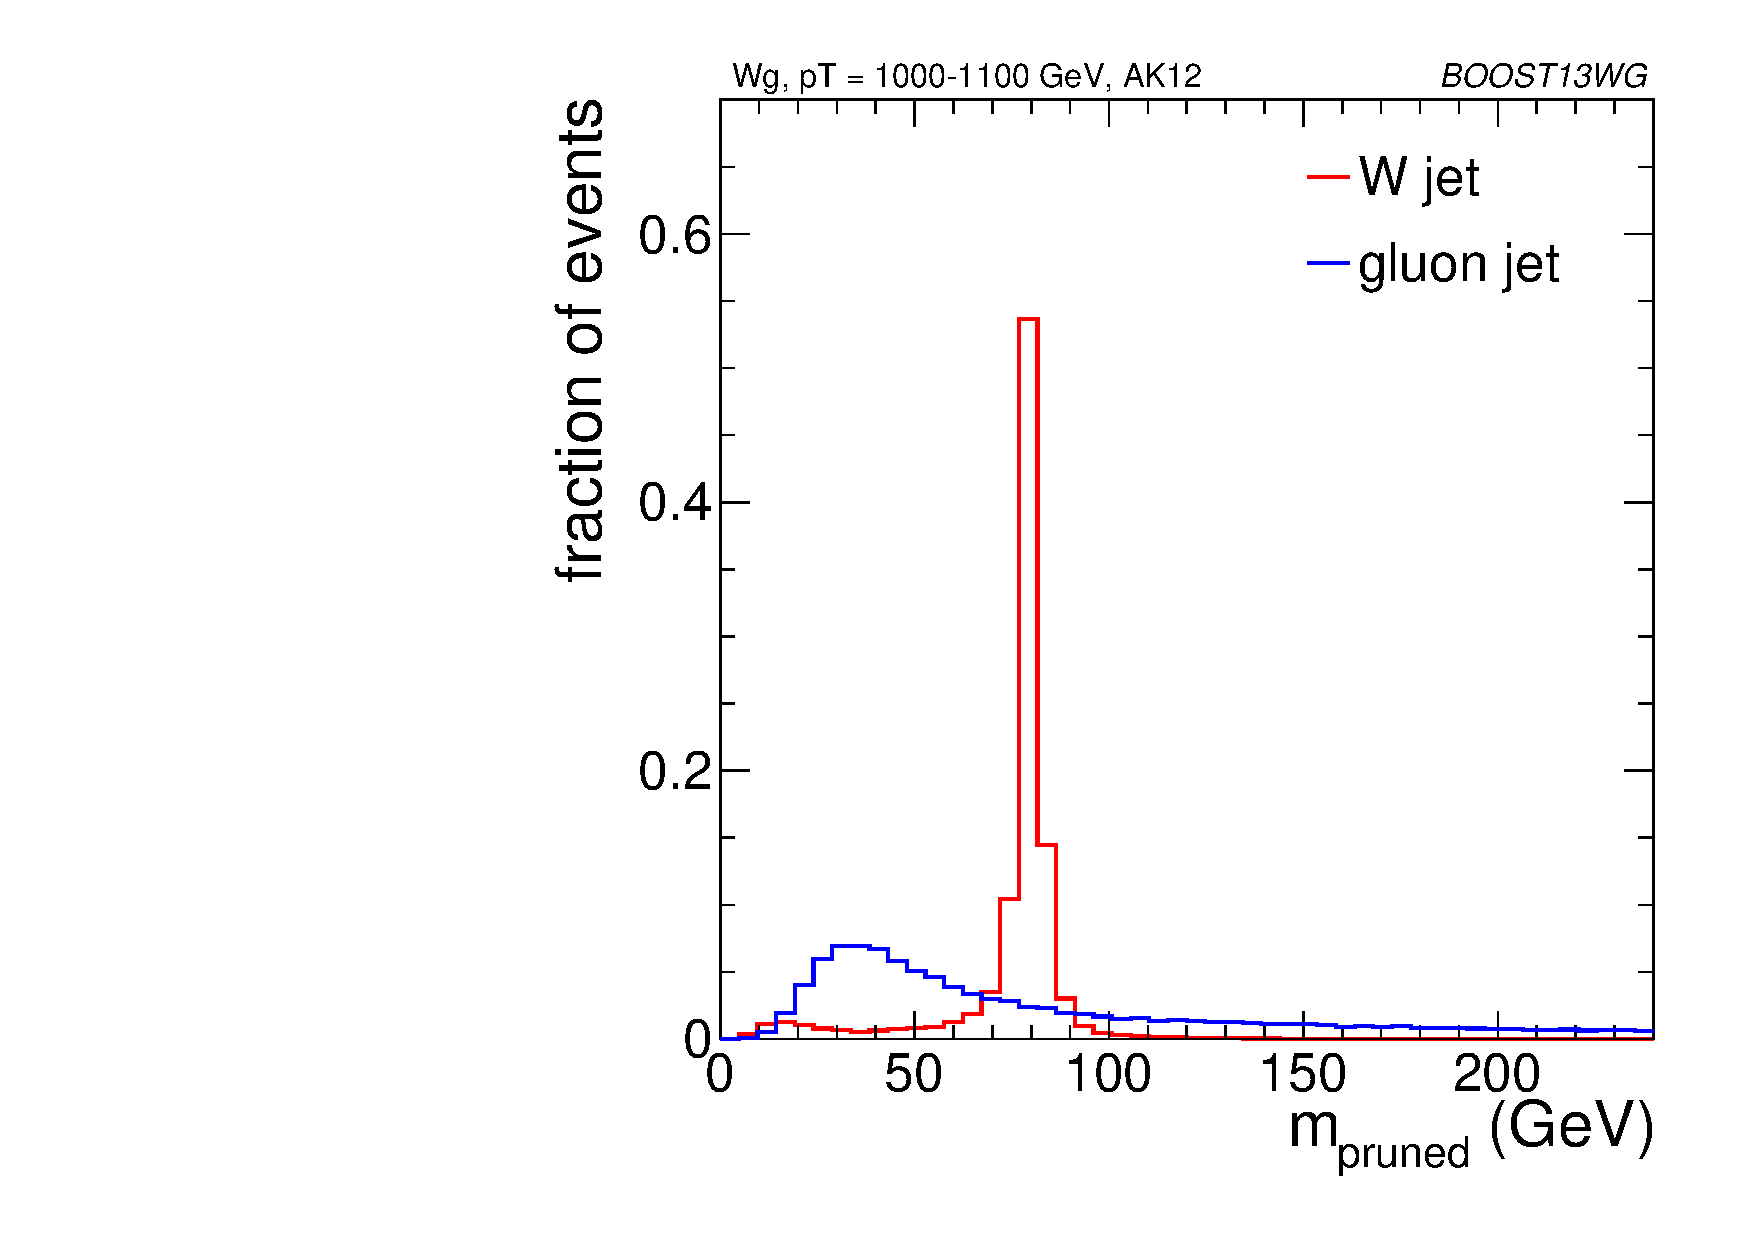
\includegraphics[width=0.4\textwidth]{./Figures/WTagging/pT1000/AKtR12/h_mass_prun.pdf}}
\caption{The Soft-drop $\beta=2$ and pruned groomed mass distribution for signal
  and background $R=1.2$ jets in two different \pt bins.}
\label{fig:ptdepend_groomedmass}
\end{figure*}


However, one can see from the Figures~\ref{fig:pt300_comb2D_12},~\ref{fig:pt500_comb2D_12}
and~\ref{fig:pt1000_comb2D_12} that the $C_2^{\beta=1}$, $\Gamma_{\rm Qjet}$ and
$\tau_{21}^{\beta=1}$ substructure variables behave somewhat
differently. The background rejection power of the $\Gamma_{\rm Qjet}$ and
$\tau_{21}^{\beta=1}$ variables both decrease with increasing \pt, by
up to a factor two in going from the 300-400 \GeV to
1.0-1.1 \TeV bins. Conversely the rejection power of $C_2^{\beta=1}$
dramatically increases with increasing \pt for $R=0.8$, but does not
improve with \pt for the larger jet radius $R=1.2$. In Figure~\ref{fig:ptdepend_substructure} we show the
$\tau_{21}^{\beta=1}$ and $C_2^{\beta=1}$ distributions for signal and background in the \pt
300-400 \GeV and \pt = 1.0-1.1 \TeV bins for $R=0.8$ jets. For
$\tau_{21}^{\beta=1}$ one can see that, in moving from  lower to 
higher \pt bins, the signal peak remains fairly unchanged, whereas the
background peak shifts to smaller $\tau_{21}^{\beta=1}$ values,
reducing the discriminating power of the variable. This is expected,
since jet substructure methods explicitly relying on the identification of hard
prongs would expect to work best at low \pt, where the prongs would
tend to be more separated. However, $C_2^{\beta=1}$ does not rely on
the explicit identification of subjets, and one can see from
Figure~\ref{fig:ptdepend_substructure} that the discrimination power
visibly increases with increasing \pt. This is in line with the
observation in \cite{Larkoski:2013eya} that $C_2^{\beta=1}$ performs best when $m/\pt$ is small.

\begin{figure*}
\centering
\subfigure[\antikt $R=0.8$, \pt = 300-400 \GeV bin]{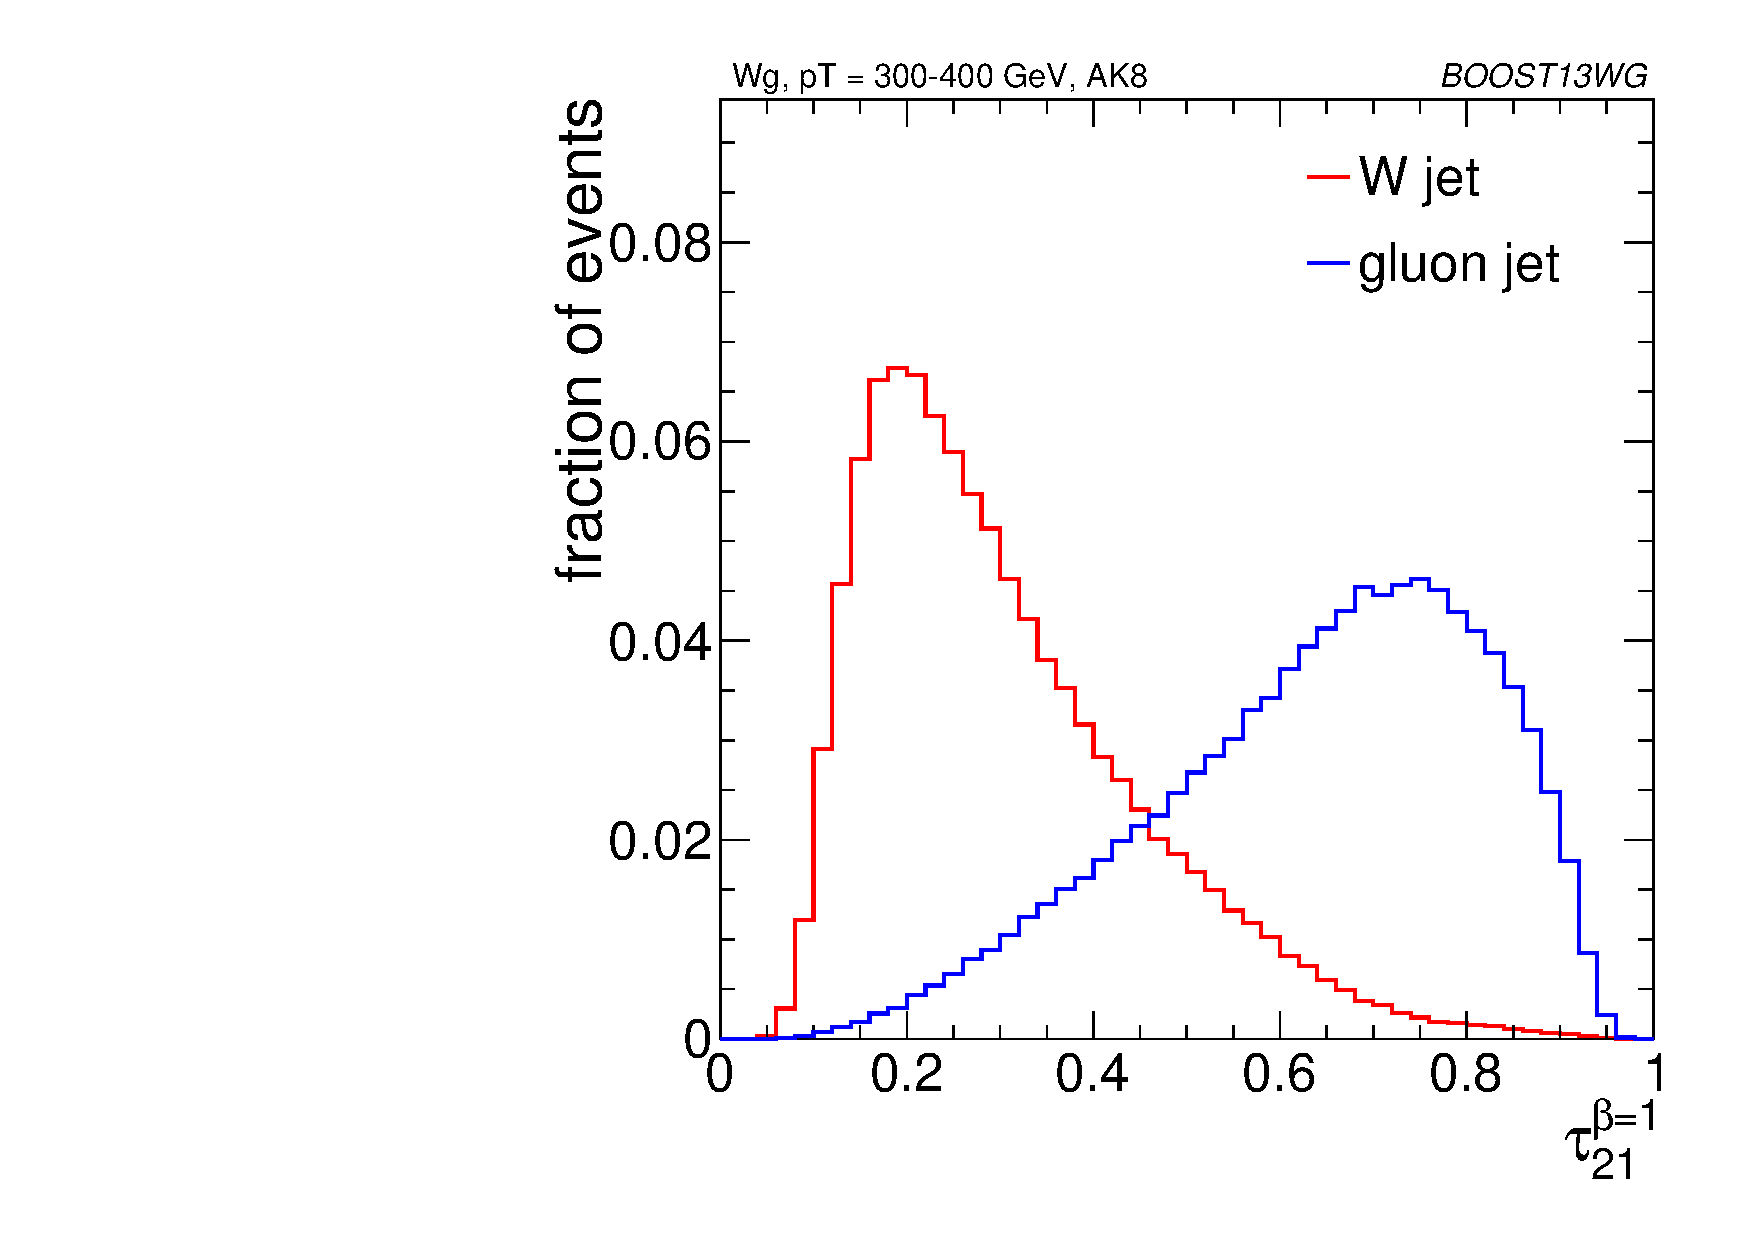
\includegraphics[width=0.4\textwidth]{./Figures/WTagging/pT300/AKtR08/h_tau21_b1.pdf}}
\subfigure[\antikt $R=0.8$, \pt = 1.0-1.1 \TeV bin]{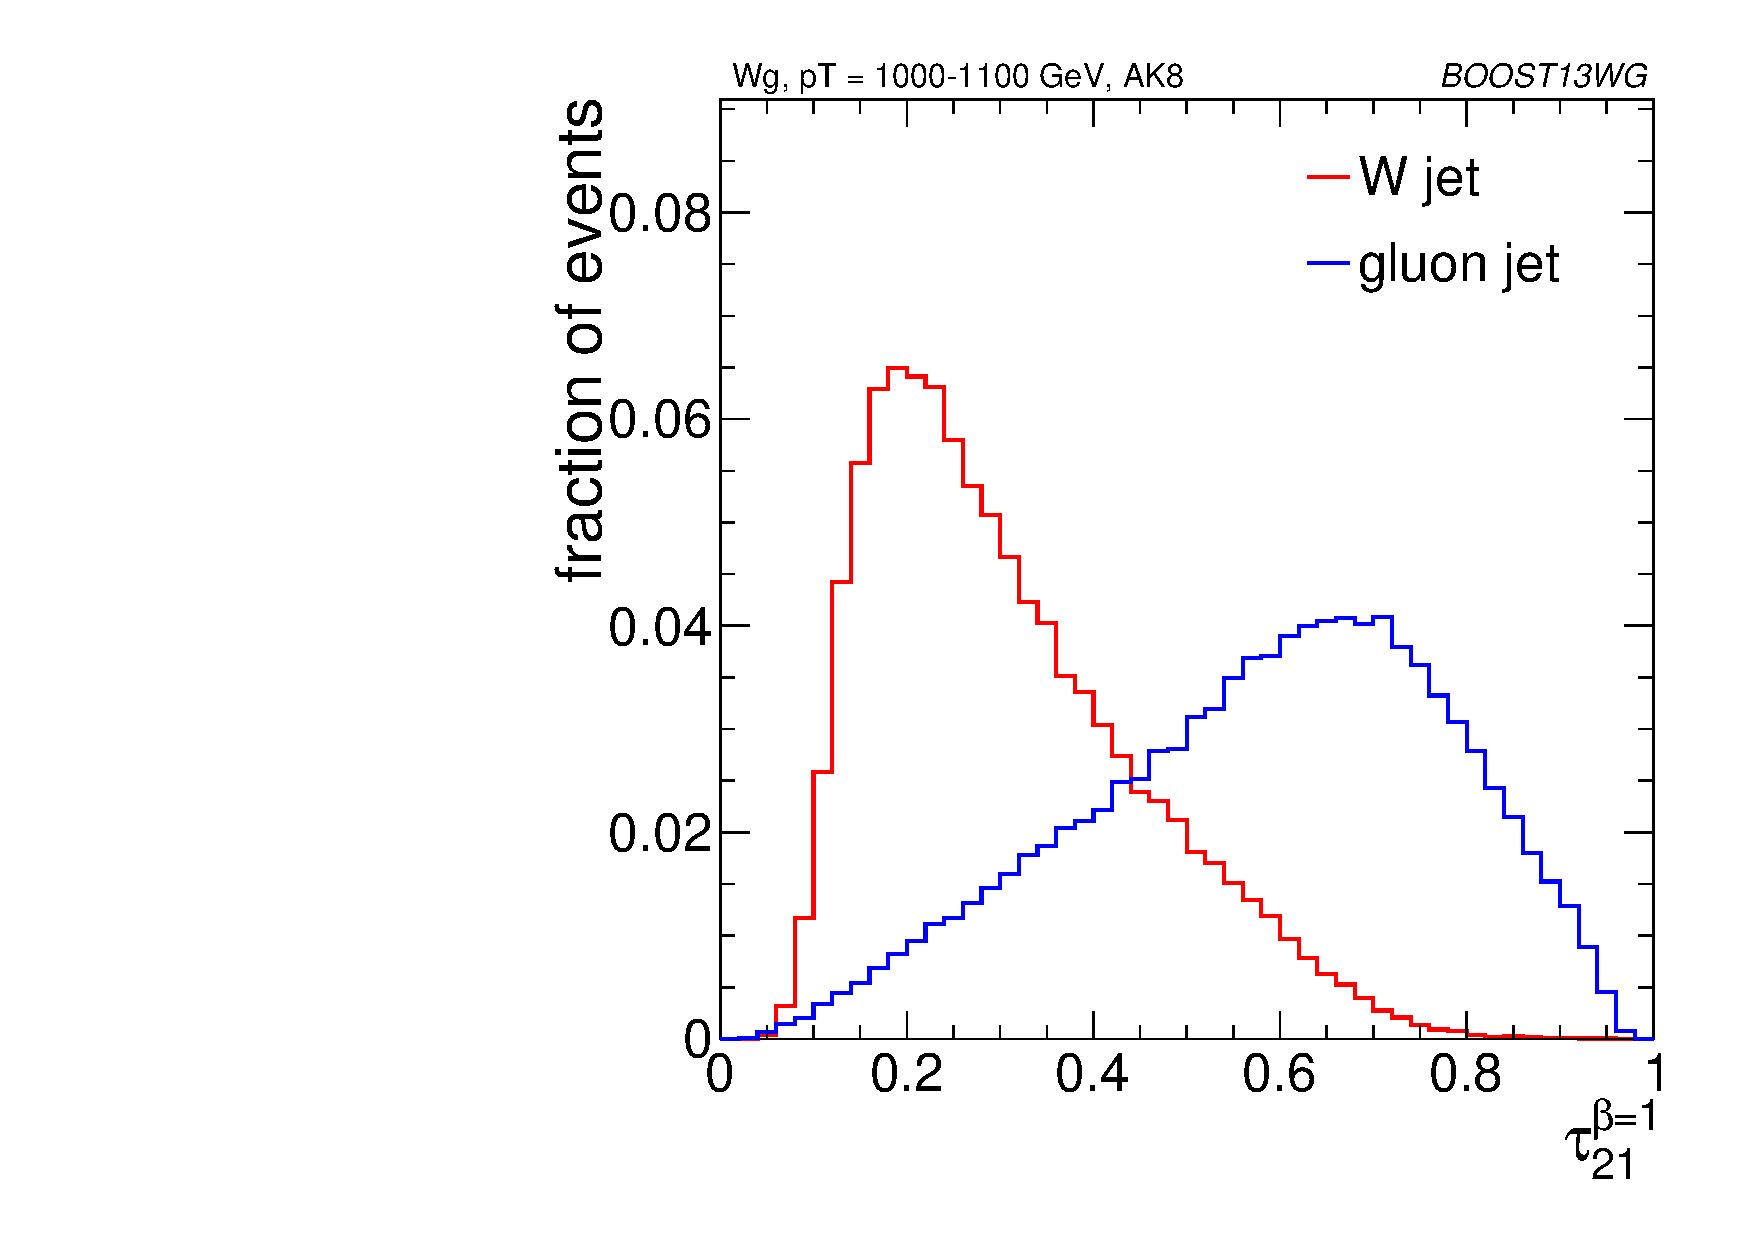
\includegraphics[width=0.4\textwidth]{./Figures/WTagging/pT1000/AKtR08/h_tau21_b1.pdf}}
\subfigure[\antikt $R=0.8$, \pt = 300-400 \GeV bin]{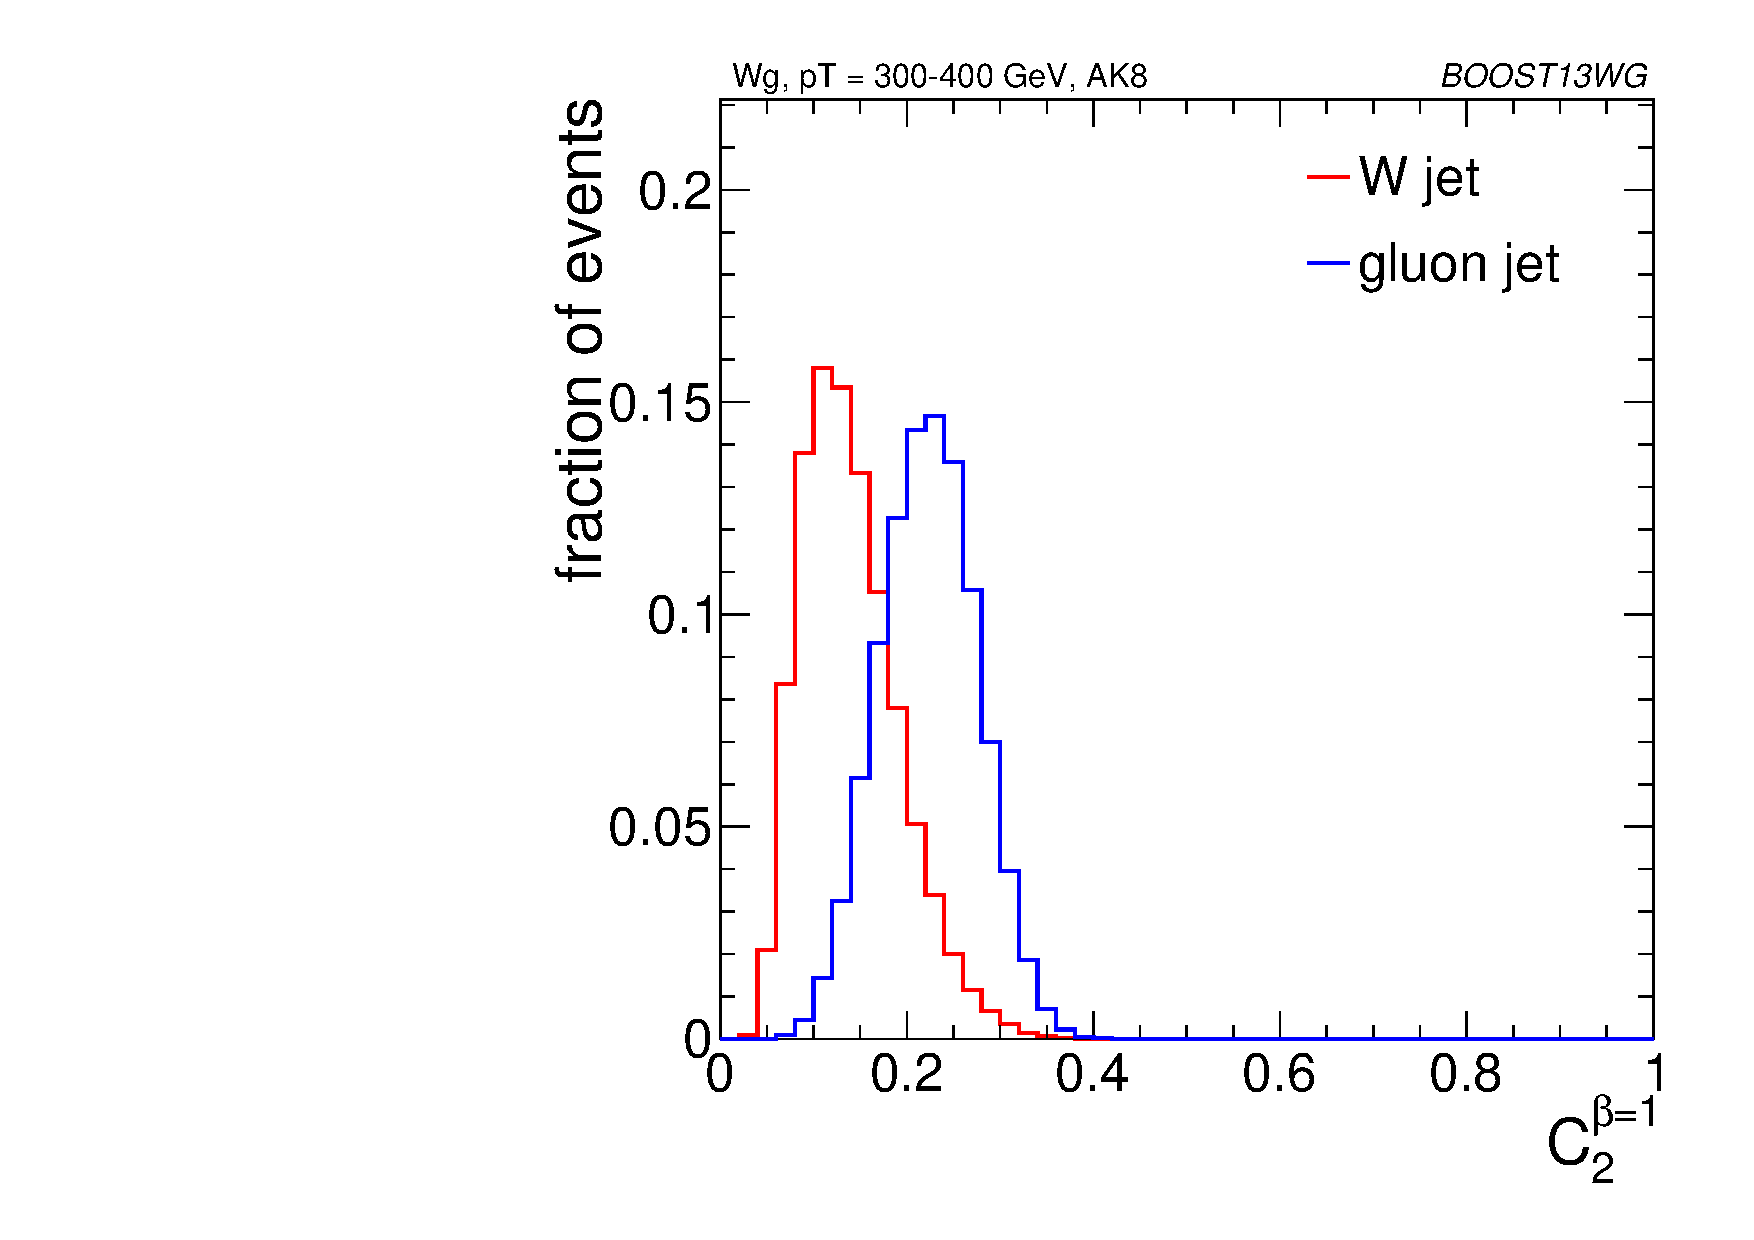
\includegraphics[width=0.4\textwidth]{./Figures/WTagging/pT300/AKtR08/h_c2_b1.pdf}}
\subfigure[\antikt $R=0.8$, \pt = 1.0-1.1 \TeV bin]{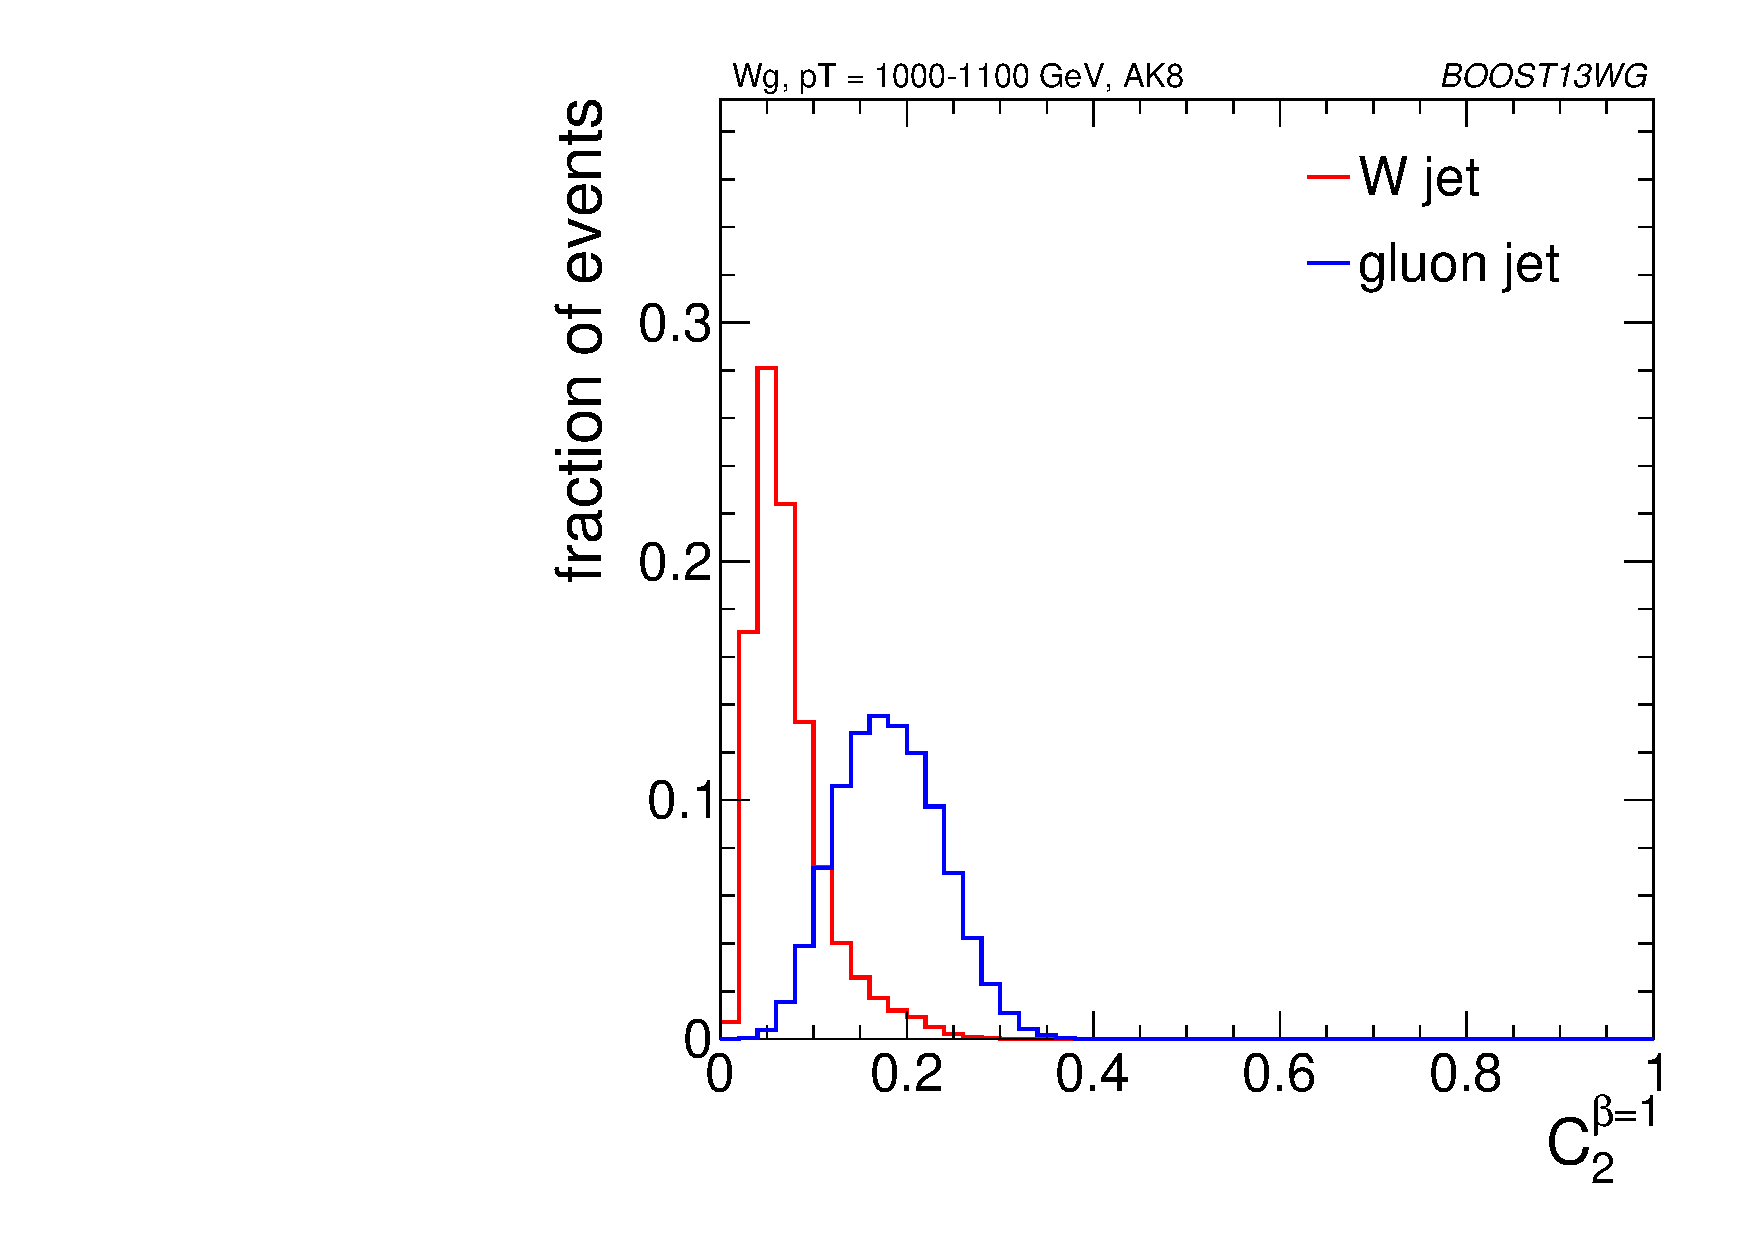
\includegraphics[width=0.4\textwidth]{./Figures/WTagging/pT1000/AKtR08/h_c2_b1.pdf}}
\caption{The $\tau_{21}^{\beta=1}$ and $C_2^{\beta=1}$ distributions for signal
  and background $R=0.8$ jets in two different \pt bins.}
\label{fig:ptdepend_substructure}
\end{figure*}

We now compare the performance of different jet radius parameters in the same \pt bin by comparing the individual sub-figures
 of Figures~\ref{fig:pt300_comb2D},~\ref{fig:pt500_comb2D}
and~\ref{fig:pt1000_comb2D}. To within
$\sim$~25\%, the background rejection power of the groomed masses remains
constant with respect to the jet
radius. Figure~\ref{fig:Rdepend_groomedmass} shows how the groomed
mass changes for varying jet radius in the \pt = 1.0-1.1 \TeV bin. One
can see that the signal mass peak remains unaffected by the increased
radius, as expected, since grooming removes the soft contamination
which could otherwise increase the mass of the jet as the radius
increased. The gluon background in the signal mass region also remains
largely unaffected, as follows from Figure~\ref{fig:qg_prmasses_log}
and the discussion in Section~\ref{sec:qg_mass},
where it is shown that there is very little dependence of the groomed gluon mass
distribution on $R$ in the signal region ($m/\pt/R \sim$ 0.5). 
%This is discussed further in Section~\ref{sec:qg_mass}.

\begin{figure*}
\centering
\subfigure[\antikt $R=0.4$, \pt = 1.0-1.1 \TeV bin]{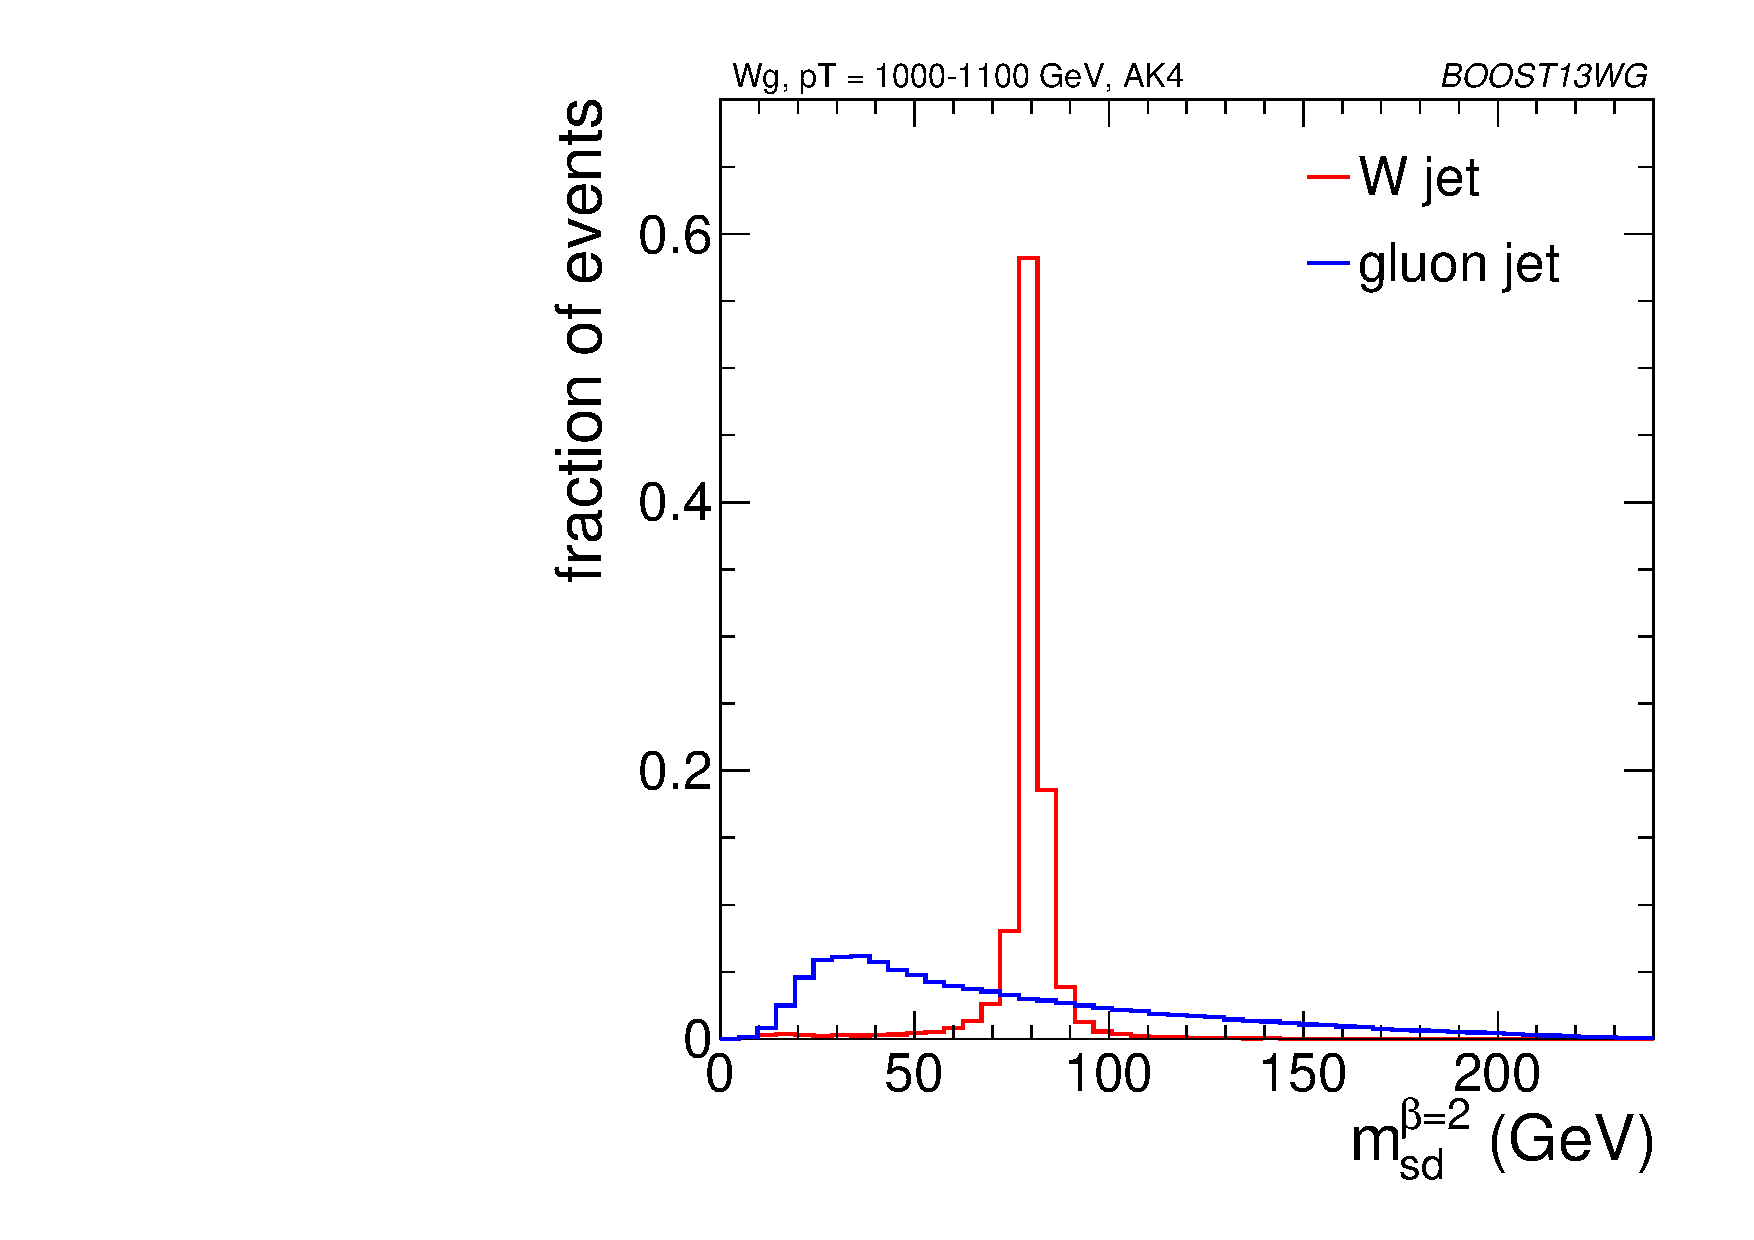
\includegraphics[width=0.4\textwidth]{./Figures/WTagging/pT1000/AKtR04/h_mass_sdb2.pdf}}
\subfigure[\antikt $R=1.2$, \pt = 1.0-1.1 \TeV bin]{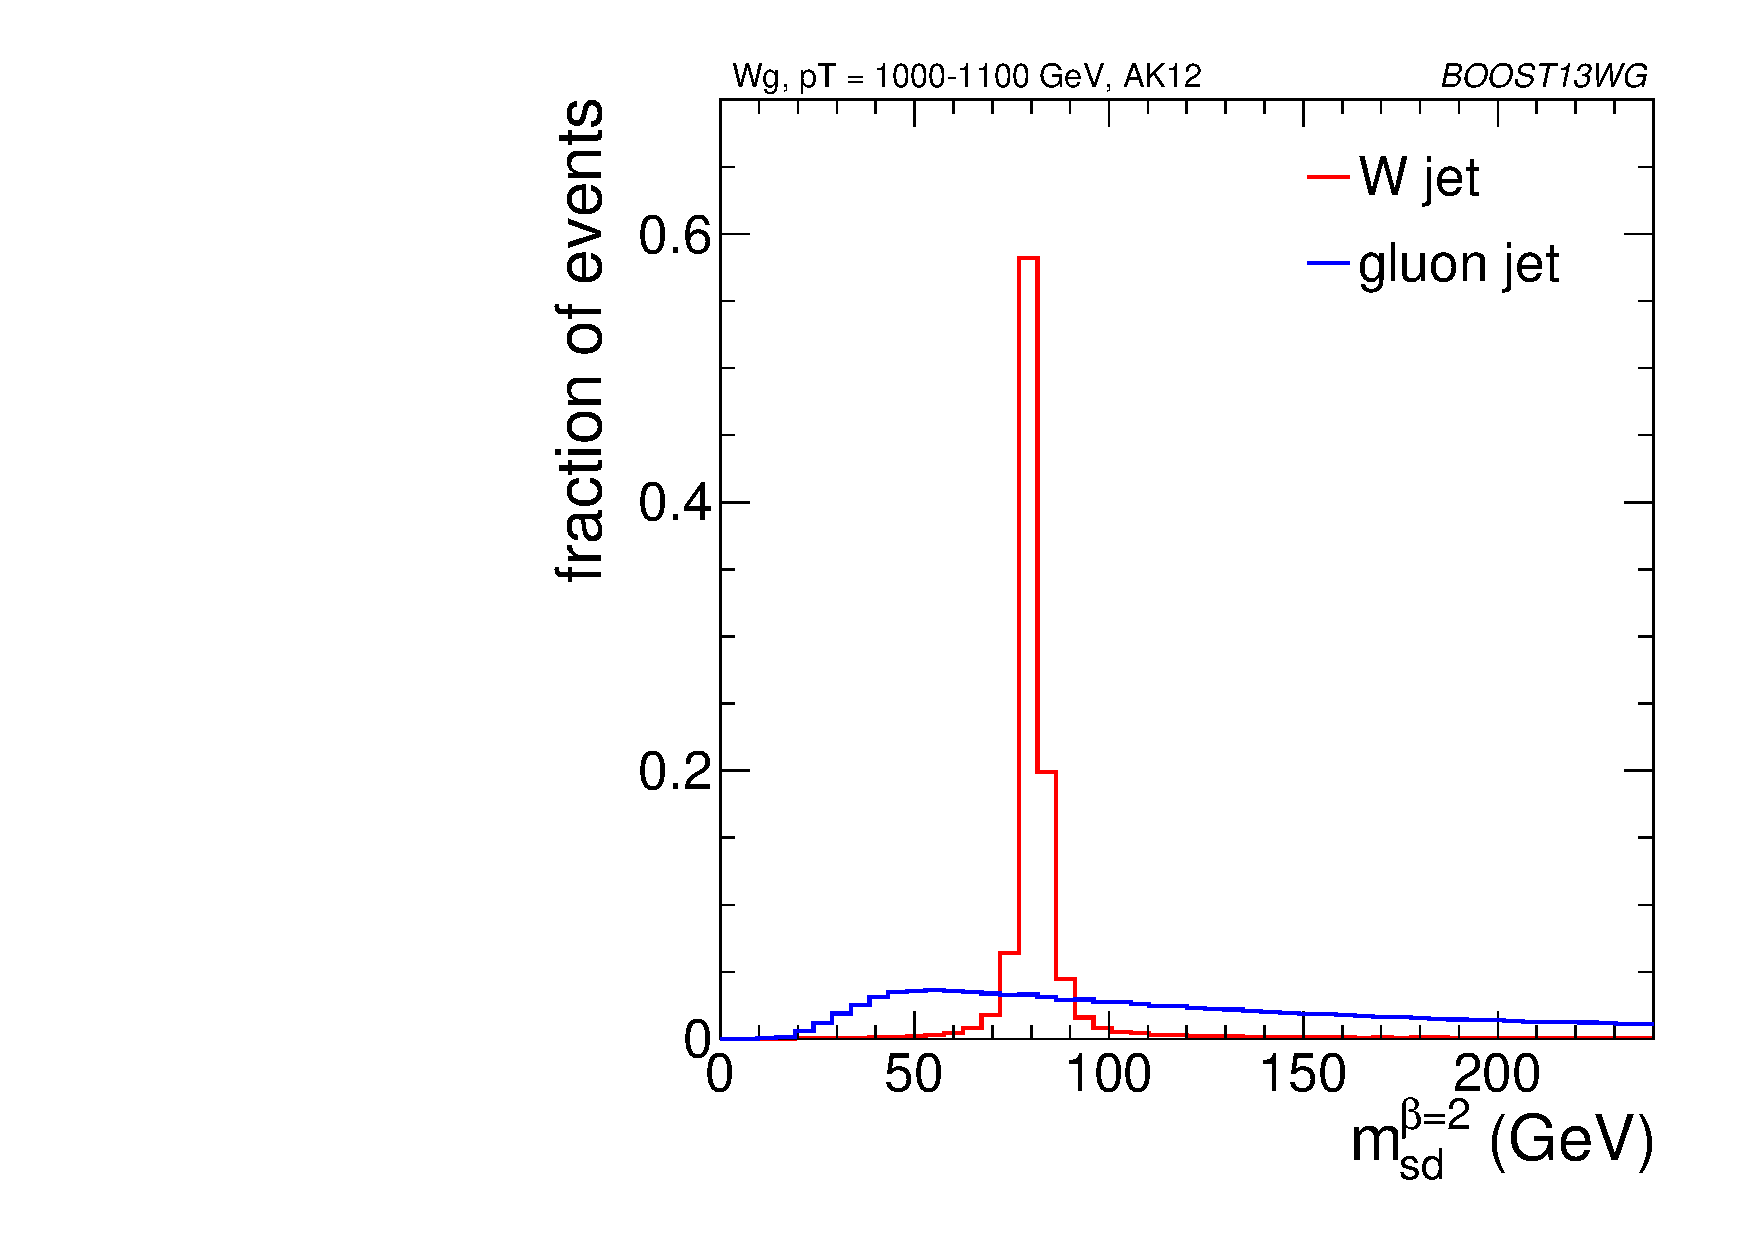
\includegraphics[width=0.4\textwidth]{./Figures/WTagging/pT1000/AKtR12/h_mass_sdb2.pdf}}
\subfigure[\antikt $R=0.4$, \pt = 1.0-1.1 \TeV bin]{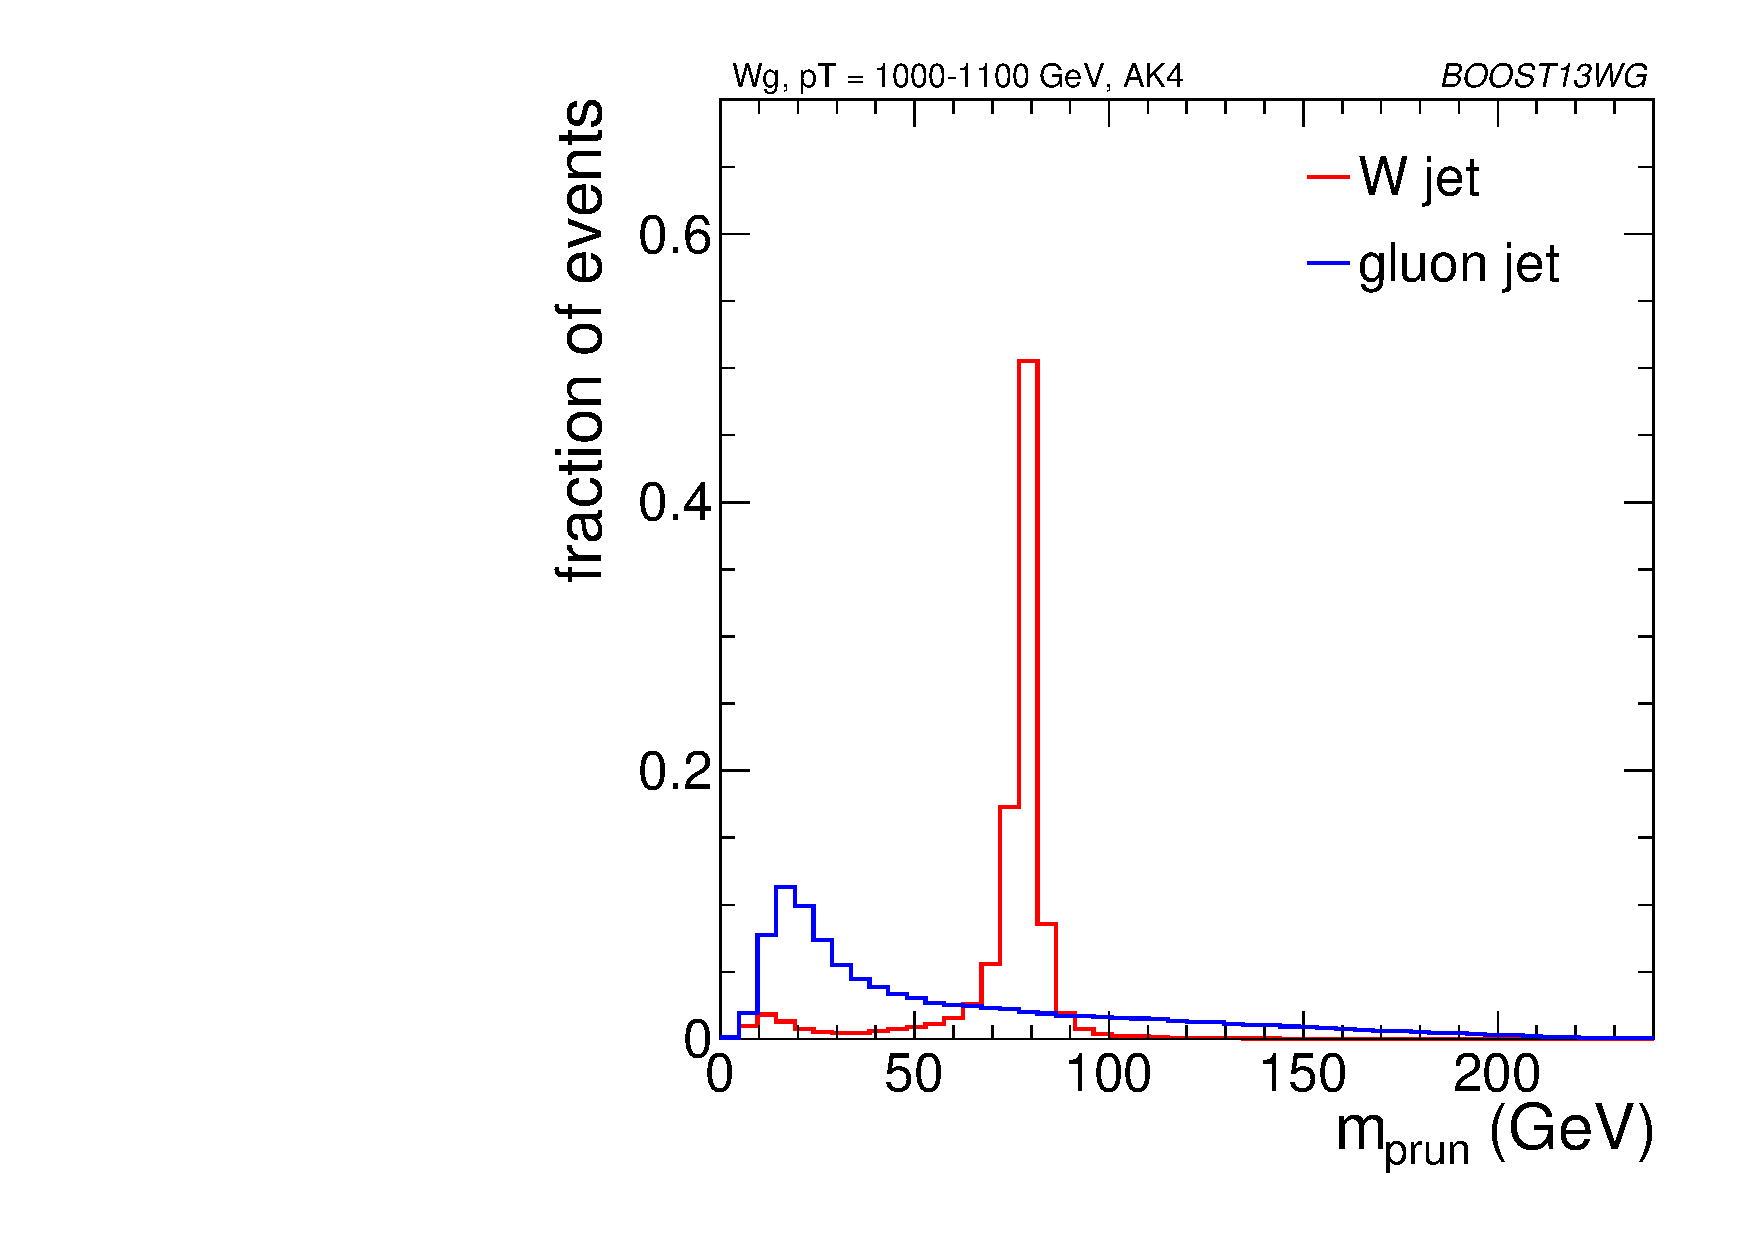
\includegraphics[width=0.4\textwidth]{./Figures/WTagging/pT1000/AKtR04/h_mass_prun.pdf}}
\subfigure[\antikt $R=1.2$, \pt = 1.0-1.1 \TeV bin]{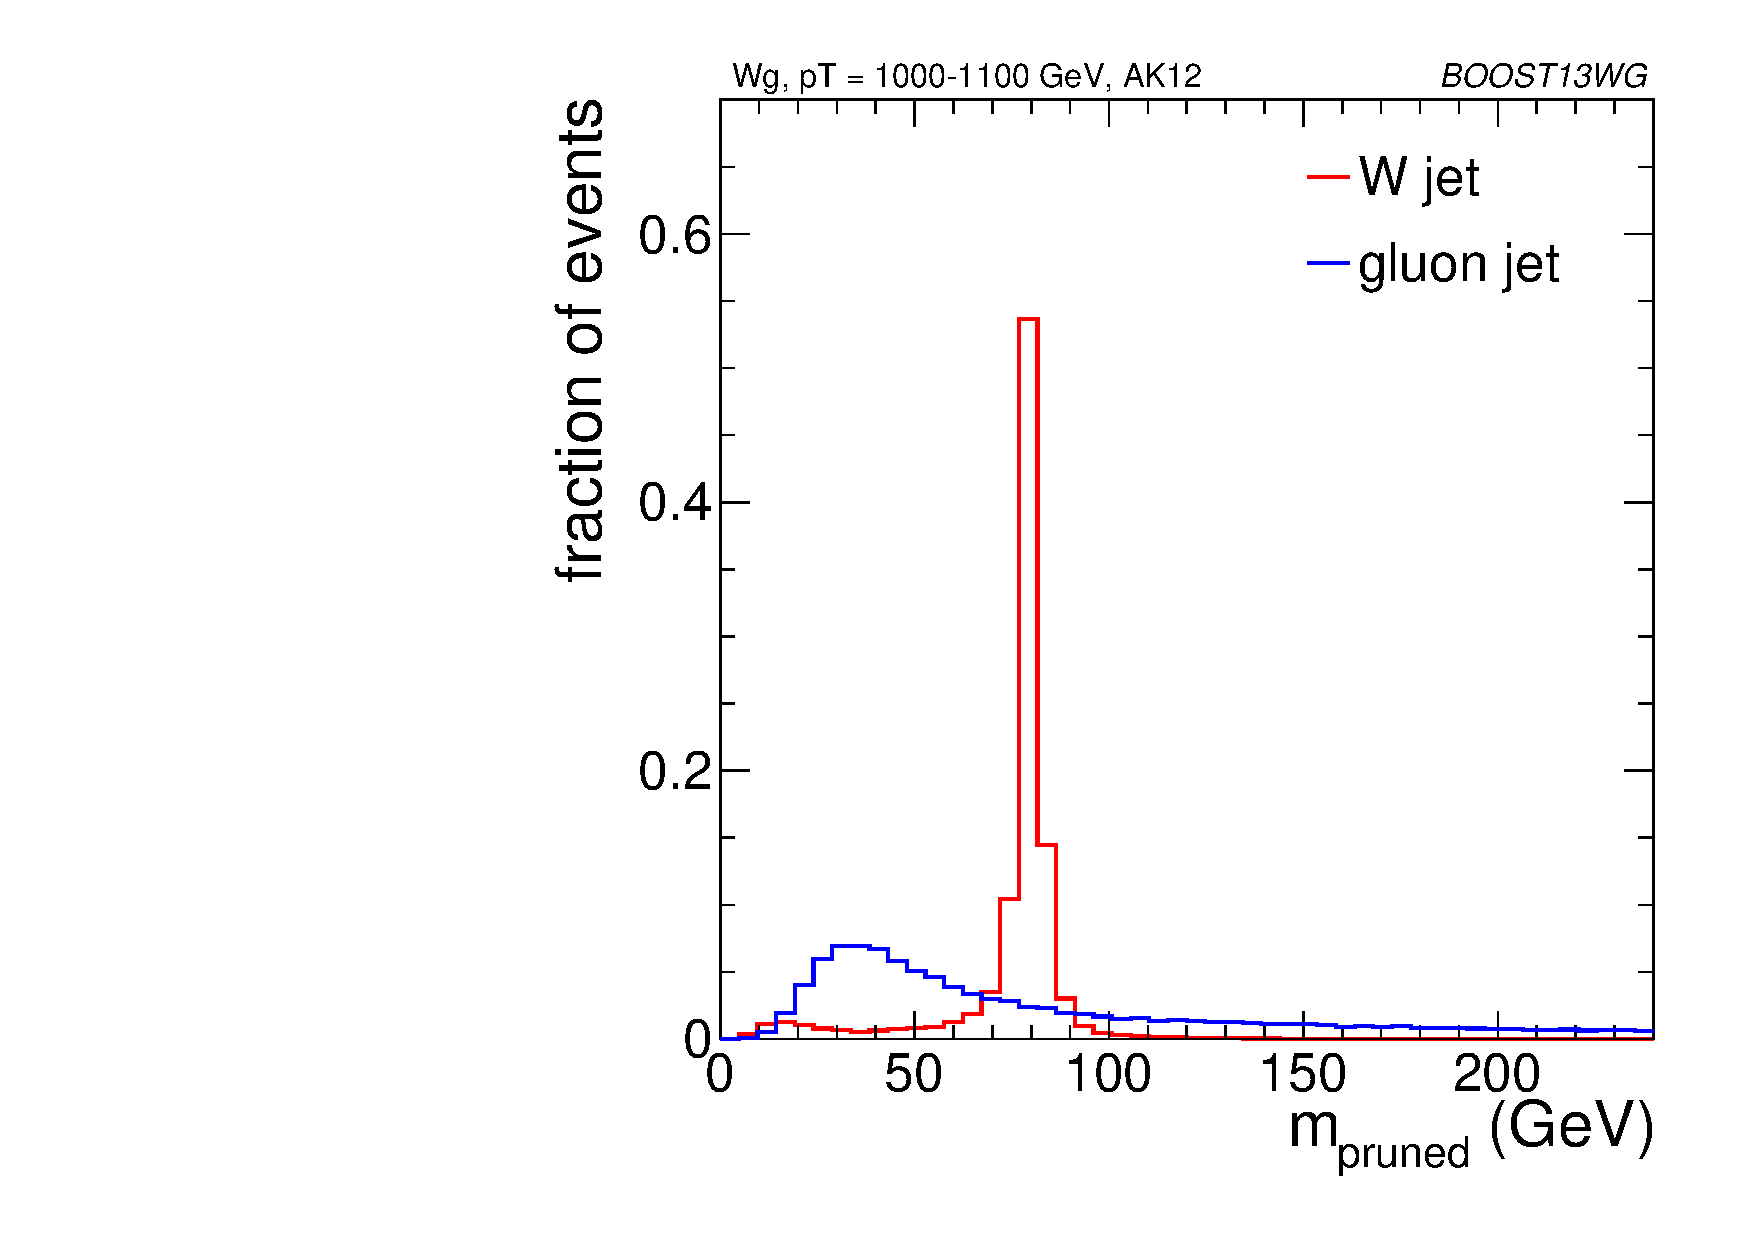
\includegraphics[width=0.4\textwidth]{./Figures/WTagging/pT1000/AKtR12/h_mass_prun.pdf}}
\caption{The Soft-drop $\beta=2$ and pruned groomed mass distribution for signal
  and background $R=0.4$ and $R=1.2$ jets in the \pt = 1.0-1.1 \TeV bin.}
\label{fig:Rdepend_groomedmass}
\end{figure*}


However, we again see rather
different behaviour versus $R$ for the substructure variables. In all \pt bins
considered, the most performant substructure variable, $C_2^{\beta=1}$,
performs best for an \antikt distance parameter of $R=0.8$. The
performance of this variable is dramatically worse for the larger jet
radius of $R=1.2$ (a factor seven worse background rejection in
the \pt = 1.0-1.1 \TeV bin), and substantially worse for $R=0.4$. For the other
jet substructure variables considered, $\Gamma_{\rm Qjet}$ and
$\tau_{21}^{\beta=1}$, their background rejection
power also reduces for larger jet radius, but not to the same
extent. Figure~\ref{fig:Rdepend_substructure} shows the
$\tau_{21}^{\beta=1}$ and $C_2^{\beta=1}$ distributions for signal and
background in the \pt = 1.0-1.1 \TeV bin for $R=0.8$ and $R=1.2$ jet
radii. For the larger jet radius, the
$C_2^{\beta=1}$  distribution of both signal and background gets wider,
and consequently the discrimination power decreases. For
$\tau_{21}^{\beta=1}$ there is comparatively little change in the distributions
with increasing jet radius. The increased sensitivity of $C_{2}$ to
soft wide angle radiation in comparison to $\tau_{21}$ is a known
feature of this variable~\cite{Larkoski:2013eya}, and a useful feature
in discriminating coloured versus colour singlet jets. However, at
very large jet radii ($R\sim1.2$), this feature becomes
disadvantageous; the jet can pick up a significant amount of initial
state or other uncorrelated radiation, and $C_{2}$ is more sensitive
to this than is $\tau_{21}$.  This uncorrelated radiation has no (or
very little) dependence on whether the jet is $W$- or gluon-initiated, and so sensitivity to this radiation means that the discrimination power will decrease.

\begin{figure*}
\centering
\subfigure[\antikt $R=0.8$, \pt = 1.0-1.1 \TeV bin]{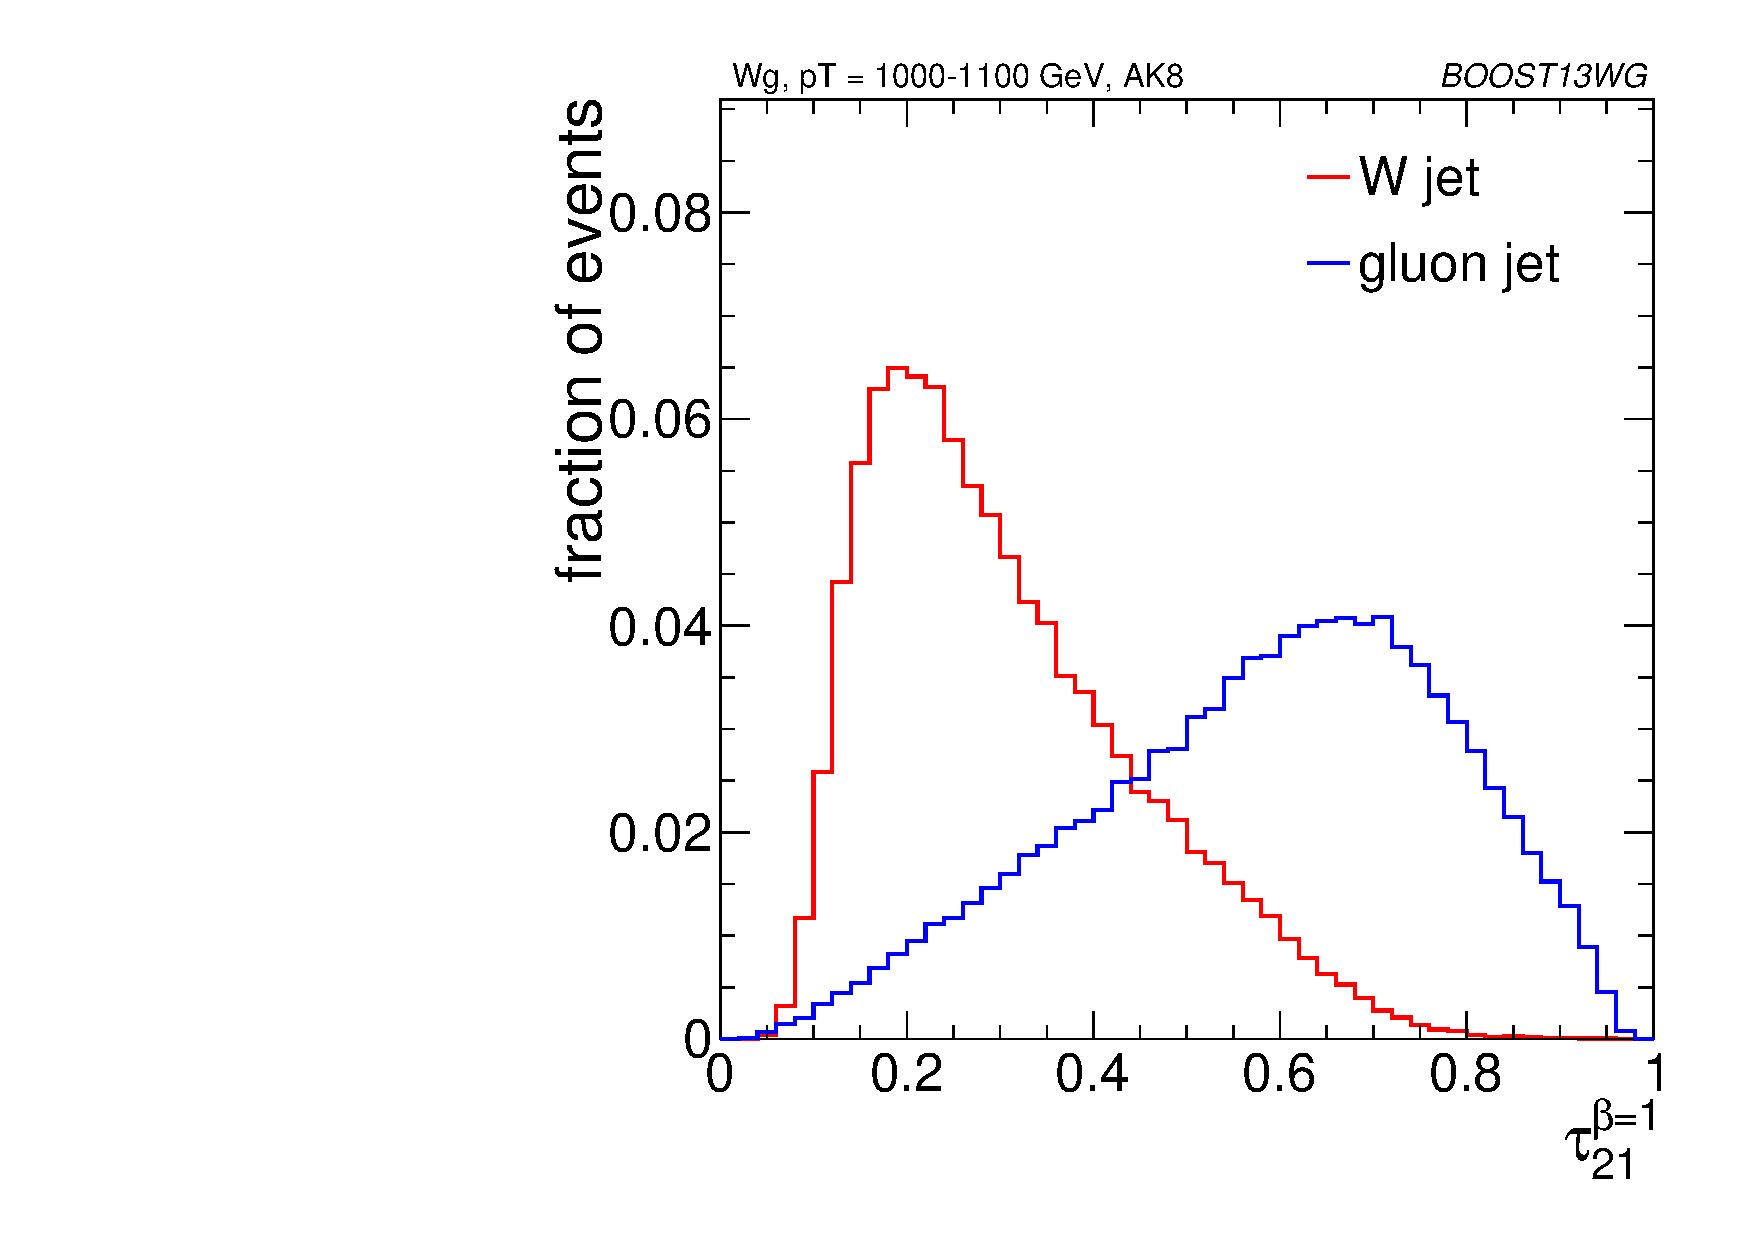
\includegraphics[width=0.4\textwidth]{./Figures/WTagging/pT1000/AKtR08/h_tau21_b1.pdf}}
\subfigure[\antikt $R=1.2$, \pt = 1.0-1.1 \TeV bin]{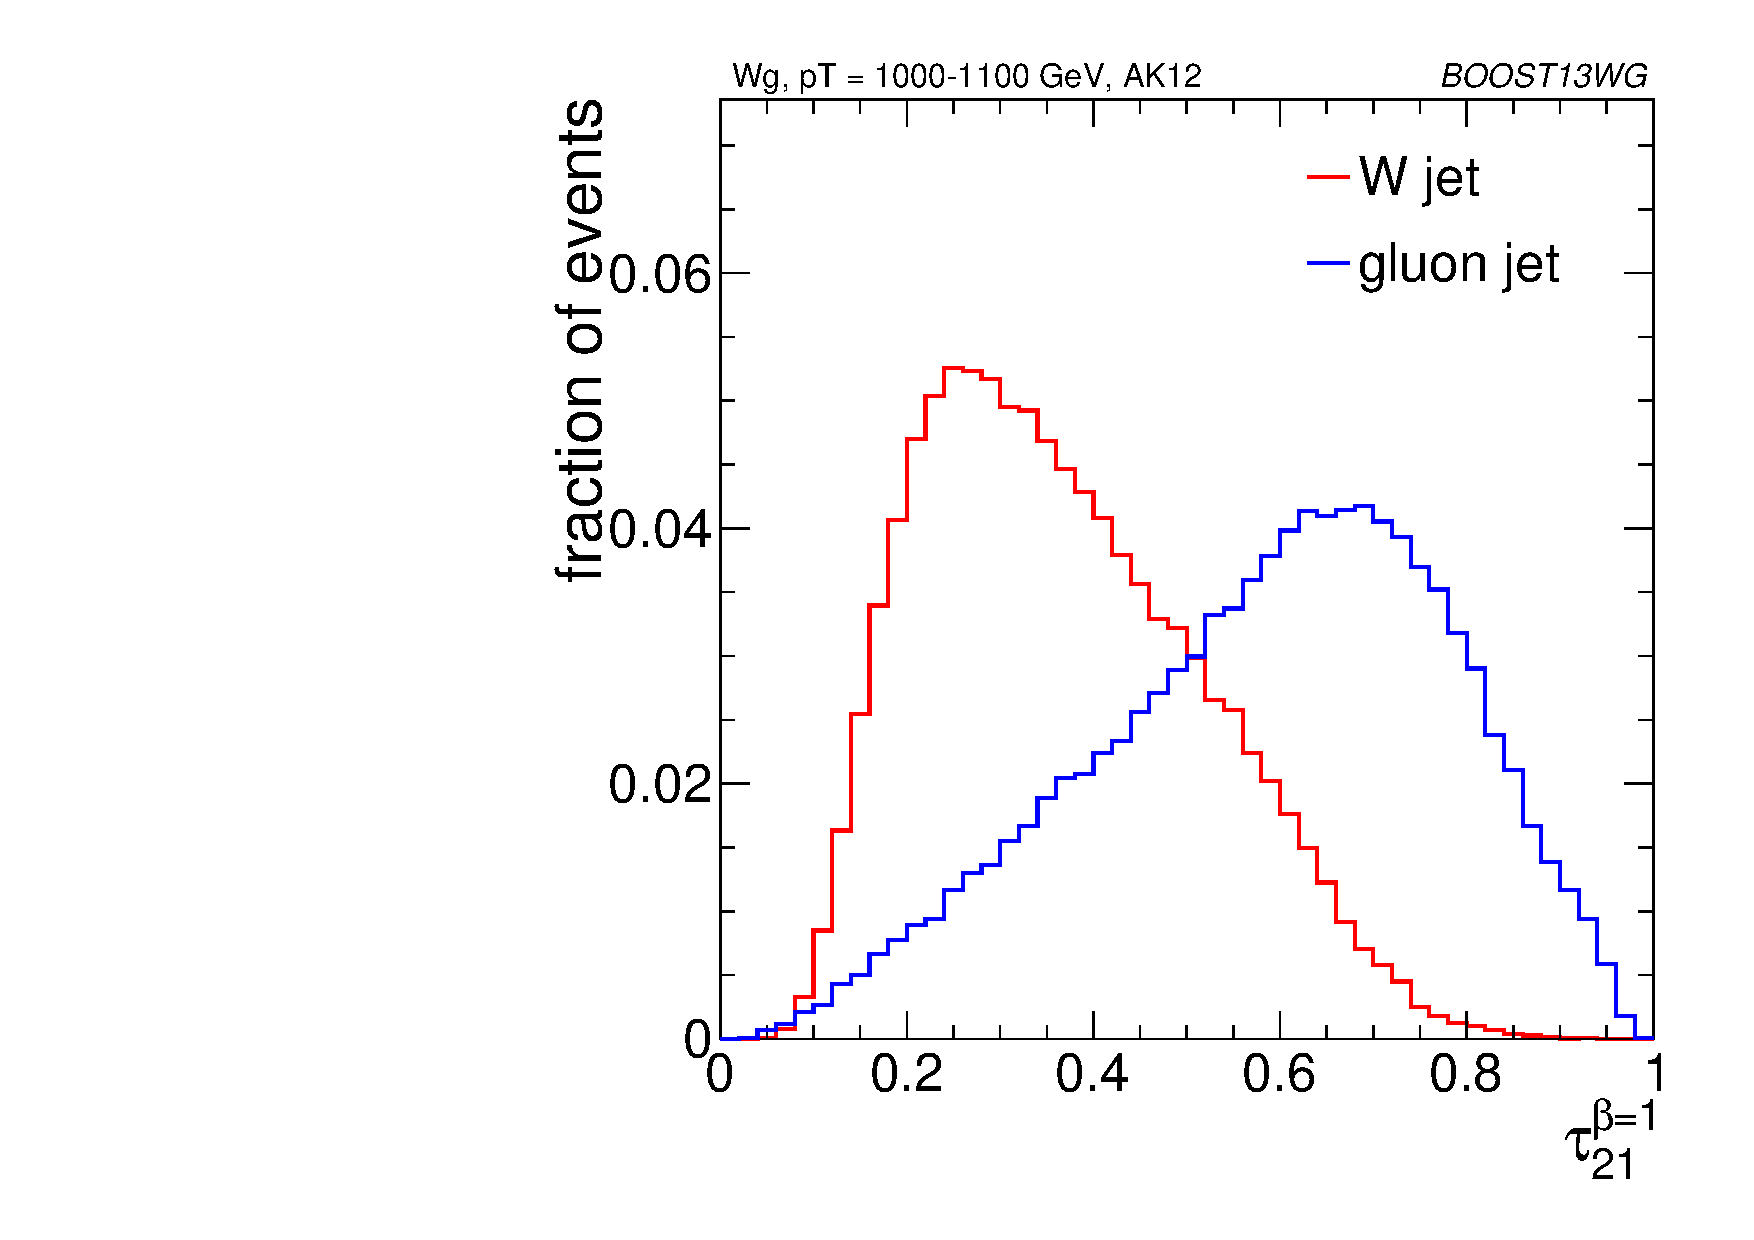
\includegraphics[width=0.4\textwidth]{./Figures/WTagging/pT1000/AKtR12/h_tau21_b1.pdf}}
\subfigure[\antikt $R=0.8$, \pt = 1.0-1.1 \TeV bin]{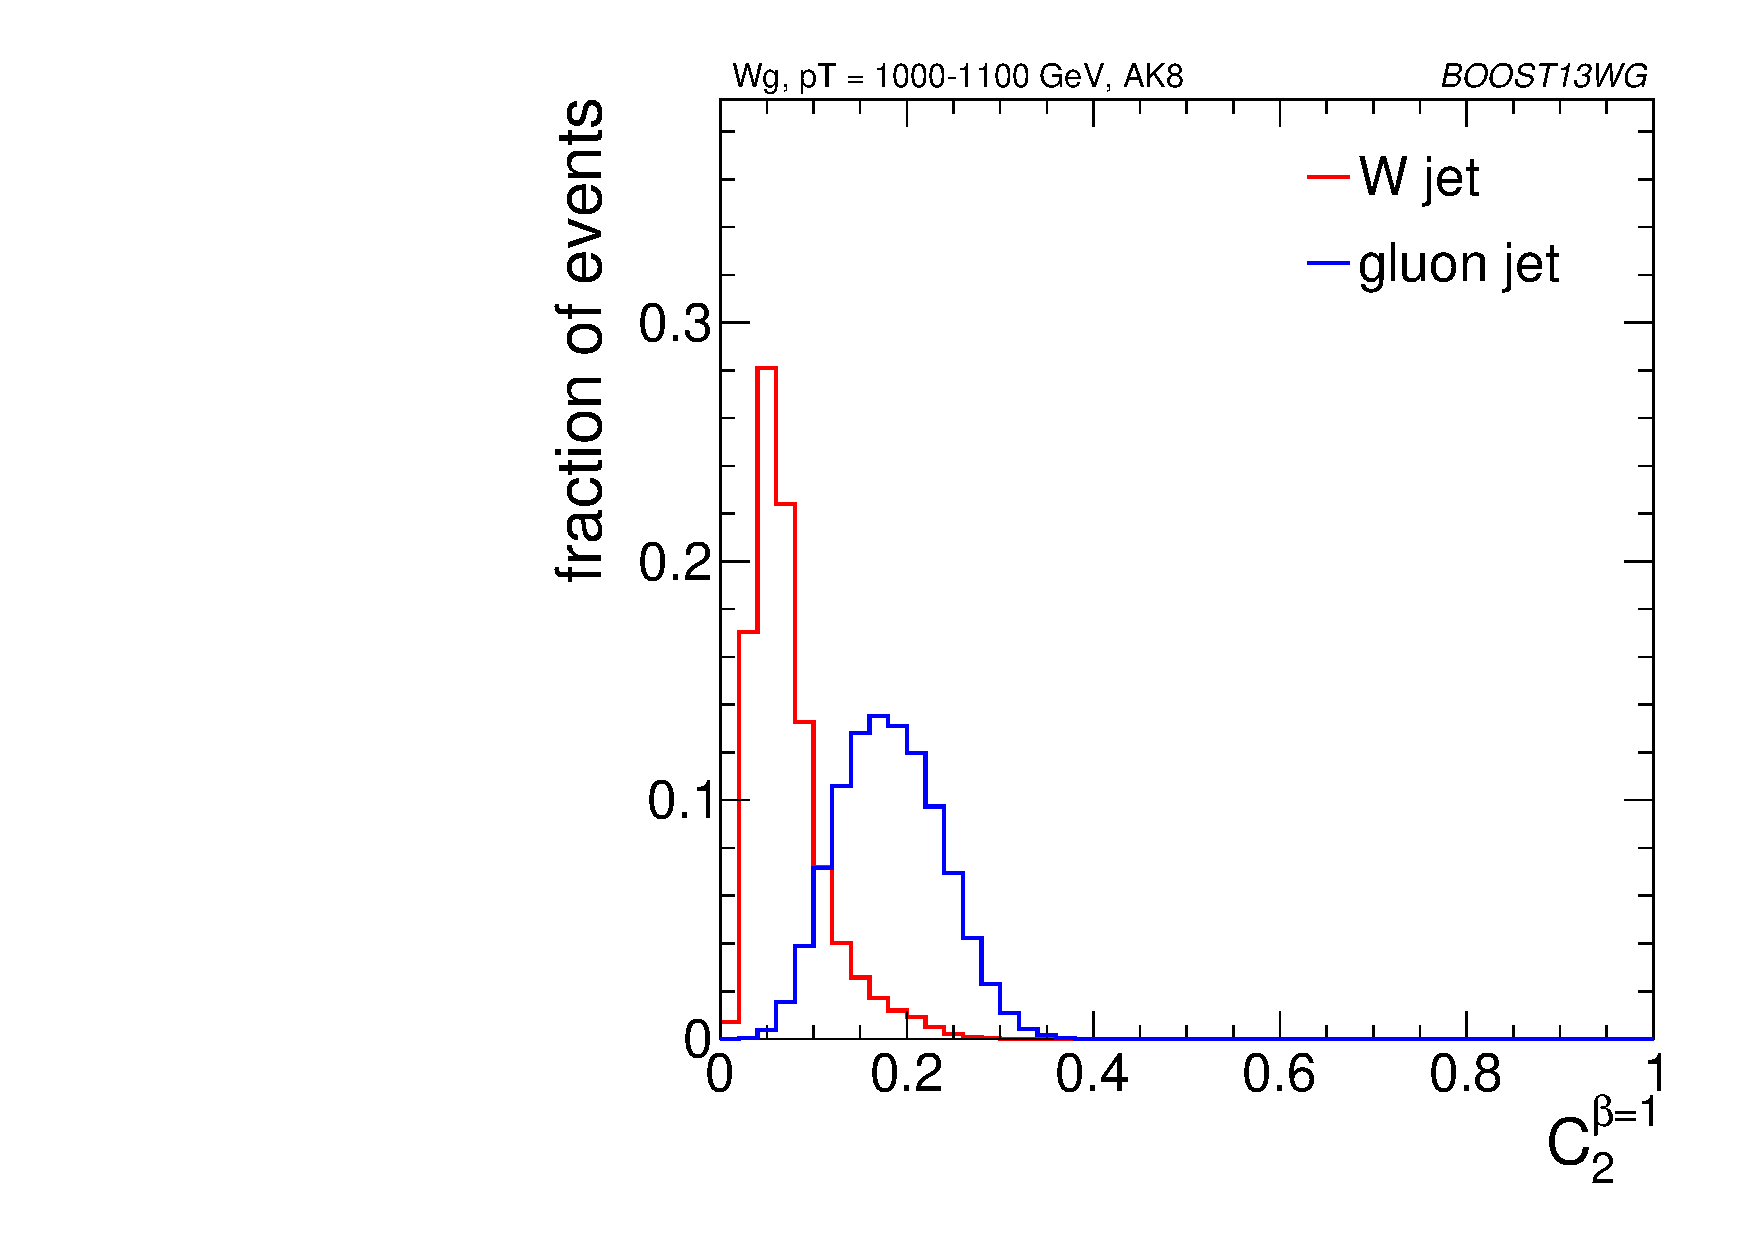
\includegraphics[width=0.4\textwidth]{./Figures/WTagging/pT1000/AKtR08/h_c2_b1.pdf}}
\subfigure[\antikt $R=1.2$, \pt = 1.0-1.1 \TeV bin]{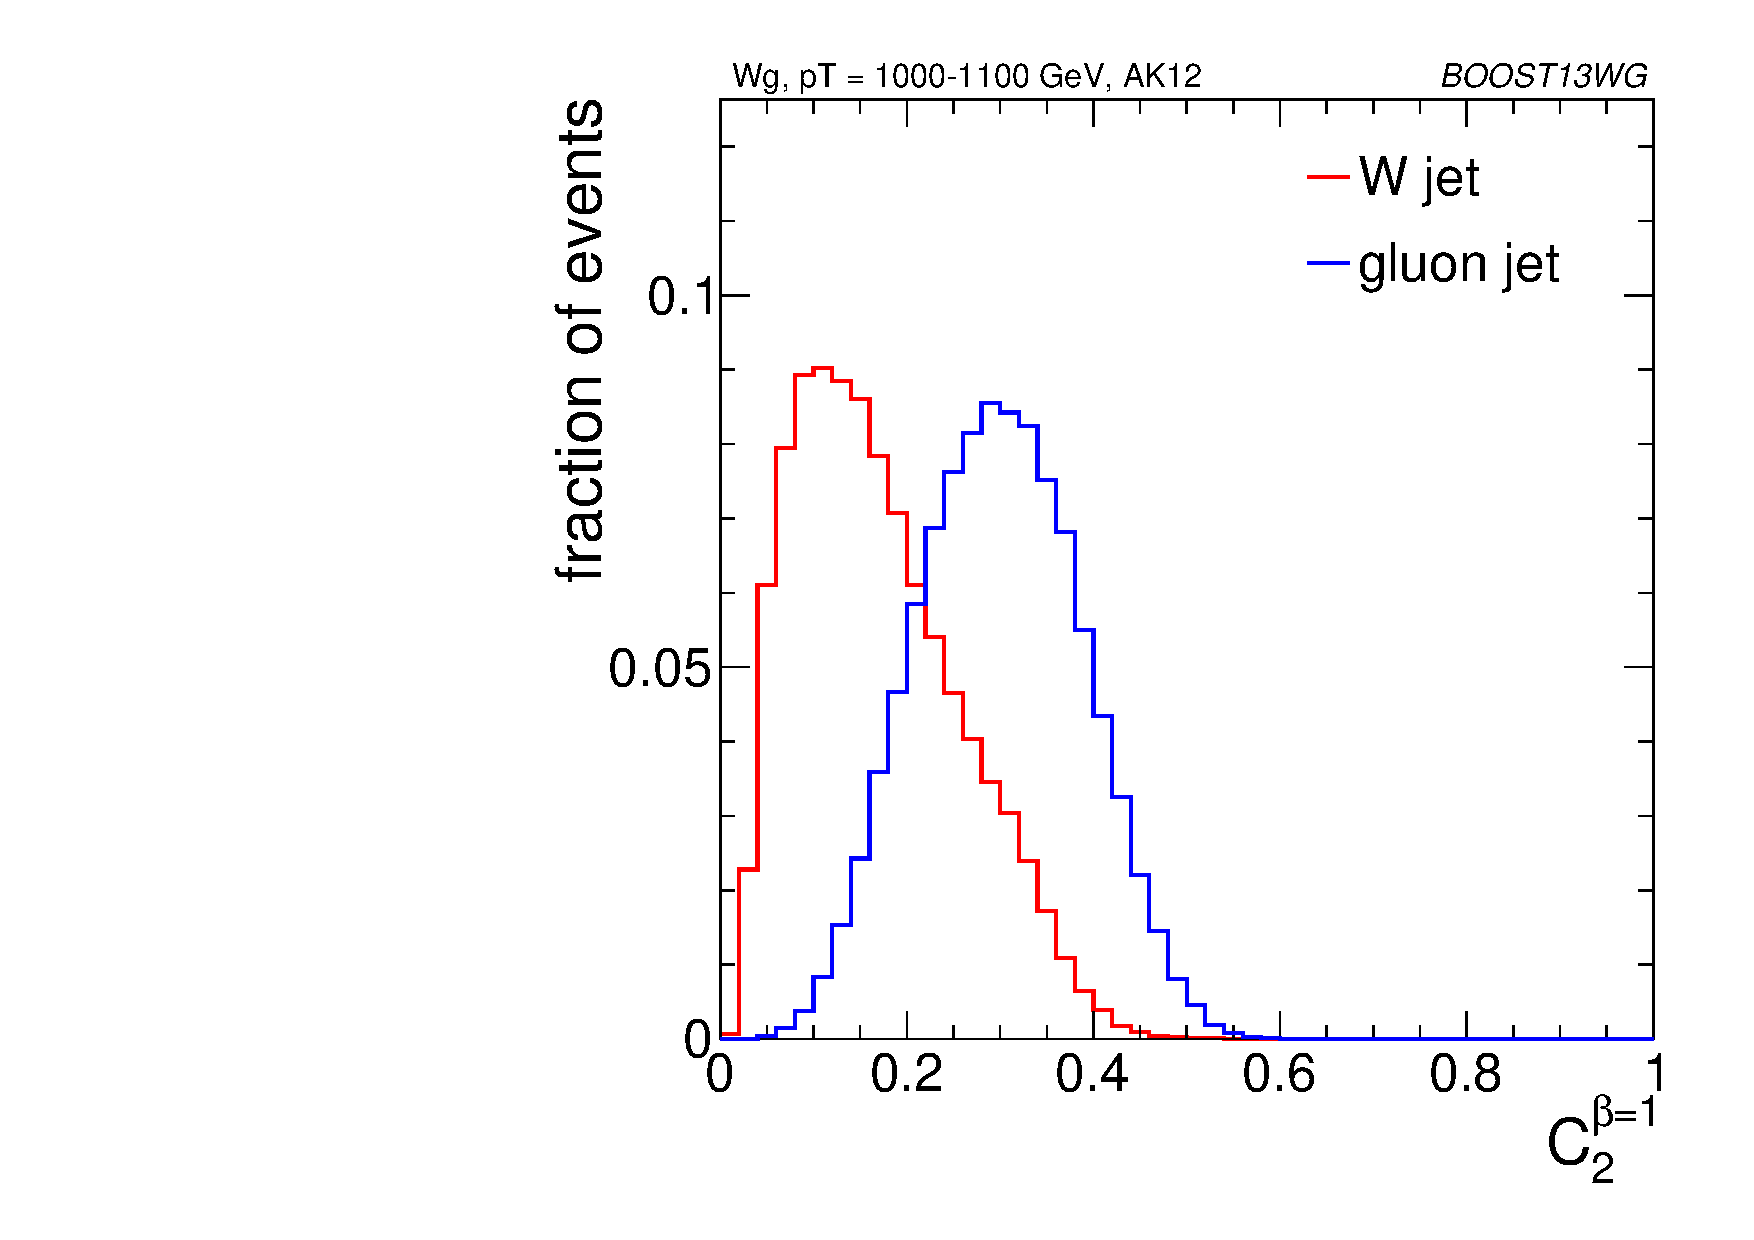
\includegraphics[width=0.4\textwidth]{./Figures/WTagging/pT1000/AKtR12/h_c2_b1.pdf}}
\caption{The $\tau_{21}^{\beta=1}$ and $C_2^{\beta=1}$ distributions for signal
  and background $R=0.8$ and $R=1.2$ jets in the \pt = 1.0-1.1 \TeV bin.}
\label{fig:Rdepend_substructure}
\end{figure*}


%The best performant individual variables for a reasonable signal
%efficiency are the groomed masses, which all have a similar
%level of performance that is superior to that of any of the
%substructure variables considered. 
%
%Because we
%have not attempted to optimise the grooming parameter settings of
%each grooming algorithm, we do not want to place too much emphasis
%here on the relative performance of the groomed masses, but instead
%look at the trends veresus \pT and R. One
%can see clearly that the background rejection power of the groomed mass
%variables increases as the \pT is increased. Within a \pT
%bin, one can also see that the groomed mass performance is rather invariant to
%changes in the jet radius. In contrast, the substructure variable
%performance varies considerably as the jet radius is changed. In
%general, the background rejection power of individual jet substructure
%variables gets worse as the jet radius is increased. The only
%exception to this is in the highest \pT bin, where the background
%rejection power of $C_2^{\beta=1}$ improves when going from jet radius
%R=0.4 to R=0.8, but then gets worse again as we go to R=1.2. {\it
%  Insert some nice discussion/explanation of why jet substructure
%  power generally gets worse as we go to large jet radius, but groomed
%mass performance does not}


\subsection{Combined Performance}\label{sec:w_combined}

Studying the improvement in performance (or lack thereof) when combining single variables into a multivariate analysis gives insight into the correlations
among jet observables. The off-diagonal entries in Figures~\ref{fig:pt300_comb2D},~\ref{fig:pt500_comb2D}
and~\ref{fig:pt1000_comb2D} can be used to compare the performance
of different BDT two-variable combinations, and see how this varies as
a function of \pt and $R$. By comparing the background rejection
achieved for the two-variable combinations to the background rejection
of the ``all variables'' BDT, one can also understand how 
discrimination can be improved by adding further variables to the
two-variable BDTs.

In general the most powerful two-variable
combinations involve a groomed mass and a non-mass substructure
variable ($C_2^{\beta=1}$, $\Gamma_{\rm Qjet}$ or
$\tau_{21}^{\beta=1}$). Two-variable combinations of the substructure
variables are not as powerful in comparison.  Which particular mass +
substructure variable combination is the most
powerful depends strongly on the \pt and $R$ of the jet, as discussed
in the sections to follow. 

%The background rejection of
%the most powerful mass + substructure combination comes very close to
%that achieved in the ``all variables'' case, indicating that there is
%little to be gained by making a BDT that is more complex, and that
%there is little more complementary information available, at least in
%terms of that which is offered by the variables considered here.

There is also modest improvement in
the background rejection when different groomed masses are combined,
 indicating that there is complementary information between the
different groomed masses. In addition, there is an improvement in the
background rejection when the groomed masses are combined with the
ungroomed mass, indicating that grooming removes some useful
discriminatory information from the jet. These observations are
explored further in the section below.

Generally, the $R=0.8$ jets offer the best two-variable
combined performance in all \pt bins explored here. This is despite
the fact that in the highest \pt = 1.0-1.1 \TeV bin the average
separation of the quarks from the $W$ decay is much smaller than 0.8,
and well within 0.4. This conclusion could of course be susceptible to
pile-up, which is not considered in this study. It is in marked
contrast to the $R$ dependence of the $q/g$ tagging performance
shown in Section~\ref{sec:qgtagging}, where a monotonic improvement
in performance with reducing $R$ is observed.

%\subsubsection{Dependence on \pt and R}
\subsubsection{Mass + Substructure Performance}
%maybe change title to "Mass + Substructure Performance"
%then can have a final section titled "All Variables Performance"

As already noted, the largest background rejection at 70\% signal
efficiency are in general achieved using those two-variable BDT combinations
which involve a groomed mass and a non-mass substructure variable. We now investigate
the \pt and $R$ dependence of the performance of these combinations.

For both $R=0.8$ and $R=1.2$ jets, the rejection power of these two-variable
combinations increases substantially with increasing \pt, at least
within the \pt range considered here.

For a jet radius of $R=0.8$, across the full \pt range considered, the
groomed mass + substructure variable combinations with the
largest background rejection are those which
involve $C_2^{\beta=1}$. For example, in combination with
\msd, this produces a five-, eight- and fifteen-fold
increase in background rejection compared to using the groomed mass
alone. In Figure~\ref{fig:2d_c2b1_AKt_R08} are shown 2-D histograms of
\msd versus $C_2^{\beta=1}$ for $R=0.8$ jets in the various \pt bins
considered, for both signal and background. The relatively low degree of
correlation between \msd versus $C_2^{\beta=1}$ that
leads to these large improvements in background rejection can be
seen. What little correlation exists is rather
non-linear in nature, changing from a negative to a positive
correlation as a function of the groomed mass, something which helps
to improve the background rejection in the region of the $W$ mass peak.

\begin{figure*}
\centering
\subfigure[\pt = 300-400 \GeV]{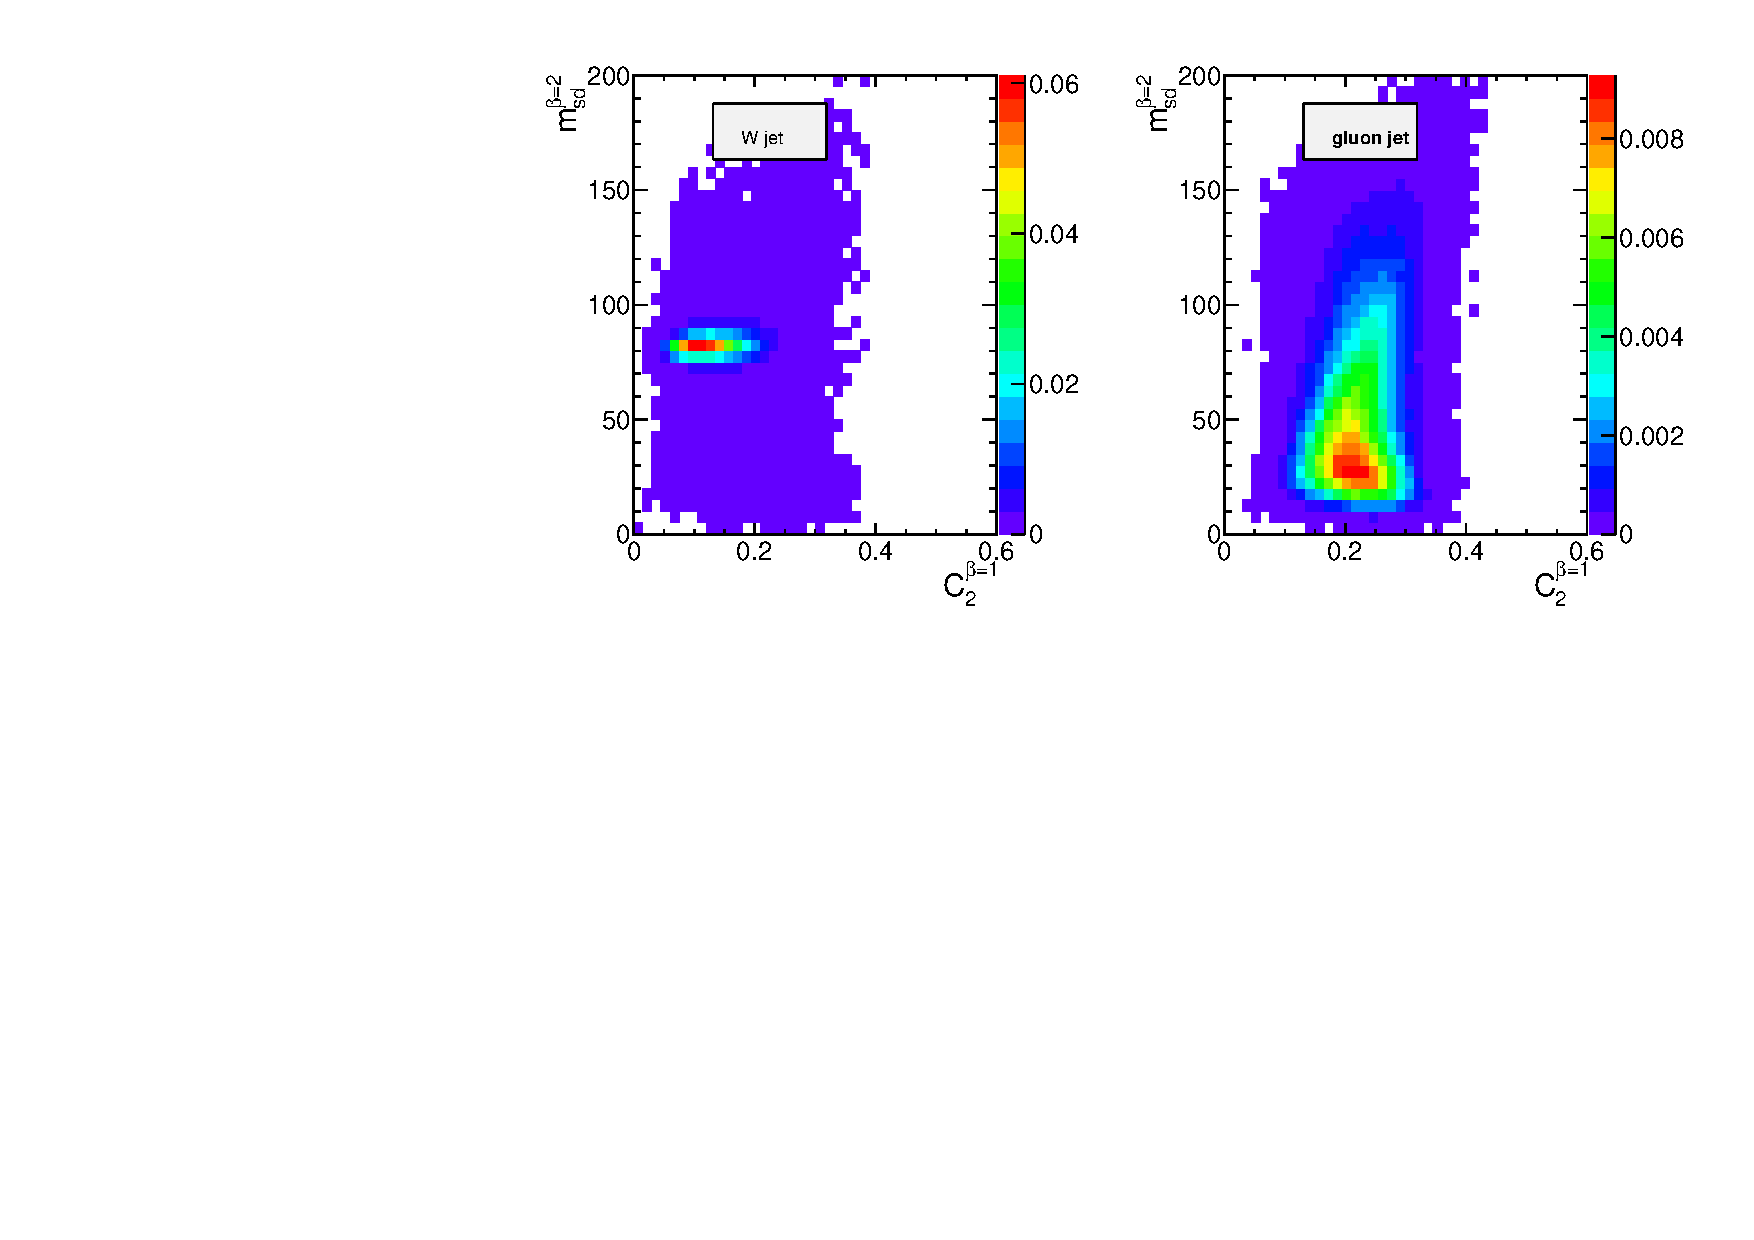
\includegraphics[width=0.78\textwidth]{./Figures/WTagging/pT300/AKtR08/h2d_jc2_b1_j_mass_sdb2_WW_onSame.pdf}\label{fig:pt300_2d_c2b1_AKt_R08}}
\subfigure[\pt = 500-600 \GeV]{\includegraphics[width=0.78\textwidth]{./Figures/WTagging/pT500/AKtR08/h2d_jc2_b1_j_mass_sdb2_WW_onSame.pdf}\label{fig:pt500_2d_c2b1_AKt_R08}}
\subfigure[\pt = 1.0-1.1 \TeV]{\includegraphics[width=0.78\textwidth]{./Figures/WTagging/pT1000/AKtR08/h2d_jc2_b1_j_mass_sdb2_WW_onSame.pdf}\label{fig:pt1000_2d_c2b1_AKt_R08}}
\caption{2-D histograms of $m_{sd}^{\beta=2}$ versus $C_2^{\beta=1}$
  distributions for $R=0.8$ jets in the various \pt bins considered, shown separately for signal and background.}
\label{fig:2d_c2b1_AKt_R08}
\end{figure*}


However, when we switch to a jet radius of $R=1.2$ the picture for
$C_2^{\beta=1}$ combinations changes dramatically. These become
significantly less powerful, and the most powerful variable in groomed
mass combinations becomes $\tau_{21}^{\beta=1}$ for all jet
\pt considered. Figure~\ref{fig:2d_c2b1_pt1000} shows the correlation between
$m_{sd}^{\beta=2}$ and $C_2^{\beta=1}$ in the \pt = 1.0 - 1.1 \TeV bin for
the various jet radii considered. Figure~\ref{fig:2d_tau21_pt1000} is
the equivalent set of distributions for $m_{sd}^{\beta=2}$ and
$\tau_{21}^{\beta=1}$. One can see from
Figure~\ref{fig:2d_c2b1_pt1000} that, due to the sensitivity of the
observable to to soft, wide-angle radiation, as the jet radius increases
$C_2^{\beta=1}$ increases and becomes more and more smeared out for both signal and
background, leading to worse discrimination power. This does not
happen to the same extent for $\tau_{21}^{\beta=1}$. We can see from Figure~\ref{fig:2d_tau21_pt1000} that
the negative correlation between $m_{sd}^{\beta=2}$ and
$\tau_{21}^{\beta=1}$ that is clearly visible for $R=0.4$ decreases for
larger jet radius, such that the groomed mass and substructure variable
are far less correlated and $\tau_{21}^{\beta=1}$ offers improved
discrimination within a $m_{sd}^{\beta=2}$ mass window.

% all variables results


\begin{figure*}
\centering
\subfigure[$R=0.4$]{\includegraphics[width=0.78\textwidth]{./Figures/WTagging/pT1000/AKtR04/h2d_jc2_b1_j_mass_sdb2_WW_onSame.pdf}\label{fig:pt1000_2d_c2b1_AKt_R04}}
\subfigure[$R=0.8$]{\includegraphics[width=0.78\textwidth]{./Figures/WTagging/pT1000/AKtR08/h2d_jc2_b1_j_mass_sdb2_WW_onSame.pdf}\label{fig:pt1000_2d_c2b1_AKt_R08_b}}
\subfigure[$R=1.2$]{\includegraphics[width=0.78\textwidth]{./Figures/WTagging/pT1000/AKtR12/h2d_jc2_b1_j_mass_sdb2_WW_onSame.pdf}\label{fig:pt1000_2d_c2b1_AKt_R12}}
\caption{2-D histograms of $m_{sd}^{\beta=2}$ versus $C_2^{\beta=1}$
  for $R=0.4$, 0.8 and 1.2 jets in the \pt = 1.0-1.1 \TeV bin, shown separately for signal and background.}
\label{fig:2d_c2b1_pt1000}
\end{figure*}

\begin{figure*}
\centering
\subfigure[$R=0.4$]{\includegraphics[width=0.78\textwidth]{./Figures/WTagging/pT1000/AKtR04/h2d_jtau21_b1_j_mass_sdb2_WW_onSame.pdf}\label{fig:pt1000_2d_tau21_AKt_R04}}
\subfigure[$R=0.8$]{\includegraphics[width=0.78\textwidth]{./Figures/WTagging/pT1000/AKtR08/h2d_jtau21_b1_j_mass_sdb2_WW_onSame.pdf}\label{fig:pt1000_2d_tau21_AKt_R08_b}}
\subfigure[$R=1.2$]{\includegraphics[width=0.78\textwidth]{./Figures/WTagging/pT1000/AKtR12/h2d_jtau21_b1_j_mass_sdb2_WW_onSame.pdf}\label{fig:pt1000_2d_tau21_AKt_R12}}
\caption{2-D histograms of $m_{sd}^{\beta=2}$ versus $\tau_{21}^{\beta=1}$
  for $R=0.4$, 0.8 and 1.2 jets in the \pt = 1.0-1.1 \TeV bin, shown separately for signal and background.}
\label{fig:2d_tau21_pt1000}
\end{figure*}





\subsubsection{Mass + Mass Performance}

The different groomed masses and the ungroomed mass are of course not
fully correlated, and thus one can always see some kind of improvement
in the background rejection when two different mass variables are combined
in the BDT. However, in some cases the improvement can be dramatic,
particularly at higher \pt, and particularly for combinations with the
ungroomed mass. For example, in Figure~\ref{fig:pt1000_comb2D} we can
see that in the \pt =1.0-1.1 \TeV bin, the combination of pruned mass with
ungroomed mass produces a greater than eight-fold improvement in the
background rejection for $R=0.4$ jets, a greater than five-fold
improvement for $R=0.8$ jets, and a factor $\sim 2$ improvement for
$R=1.2$ jets. A similar behaviour can be seen for mMDT mass. 
In Figures~\ref{fig:pt1000_2d_masses_AKt_R04},~\ref{fig:pt1000_2d_masses_AKt_R08}
and~\ref{fig:pt1000_2d_masses_AKt_R12}, we show the 2-D correlation plots of the pruned mass versus the
ungroomed mass separately for the $WW$ signal and $gg$ background
samples in the \pt = 1.0-1.1 \TeV bin, for the various jet radii
considered. For comparison, the correlation of the trimmed mass with
the ungroomed mass, a combination that does not improve on the single
mass as dramatically, is shown. In all cases one can see that there is
a much smaller degree of correlation between the pruned mass and the
ungroomed mass in the backgrounds sample than for the trimmed mass and the ungroomed mass. This
is most obvious in Figure~\ref{fig:pt1000_2d_masses_AKt_R04}, where
the high degree of correlation between the trimmed and ungroomed mass
is expected, since with the parameters used (in particular
$R_{\rm trim} = 0.2$) we cannot expect trimming to have a significant
impact on an $R=0.4$ jet. The reduced correlation with ungroomed mass
for pruning in the background means that, once we have required that the
pruned mass is consistent with a $W$ (\emph{i.e.} $\sim 80 \GeV$), a relatively large difference
between signal and background in the ungroomed mass still remains, and
can be exploited to improve the background rejection further. In other
words, many of the background events which pass the pruned mass
requirement do so because they are shifted to lower mass (to be within
a signal mass window) by the grooming, but these events still have the
property that they look very much like background events before the
grooming. A  requirement on the groomed mass alone does not
exploit this property. Of course, the impact of pile-up, not considered in this
study, could limit the degree to which the ungroomed
mass could be used to improve discrimination in this way. 

\begin{figure*}
\centering
\subfigure[Pruned mass vs ungroomed mass]{\includegraphics[width=0.78\textwidth]{./Figures/WTagging/pT1000/AKtR04/h2d_jmass_j_mass_prun_WW_onSame.pdf}\label{fig:pt1000_2d_prun_AKt_R04}}
\subfigure[Trimmed mass vs ungroomed mass]{\includegraphics[width=0.78\textwidth]{./Figures/WTagging/pT1000/AKtR04/h2d_jmass_j_mass_trim_WW_onSame.pdf}\label{fig:pt1000_2d_trim_AKt_R04}}
\caption{2-D histograms of groomed mass versus ungroomed mass in the \pt = 1.0-1.1 \TeV bin using the
  anti-\kT $R=0.4$ algorithm, shown separately for signal and background.}
\label{fig:pt1000_2d_masses_AKt_R04}
\end{figure*}

\begin{figure*}
\centering
\subfigure[Pruned mass vs ungroomed mass]{\includegraphics[width=0.78\textwidth]{./Figures/WTagging/pT1000/AKtR08/h2d_jmass_j_mass_prun_WW_onSame.pdf}\label{fig:pt1000_2d_prun_AKt_R08}}
\subfigure[Trimmed mass vs ungroomed mass]{\includegraphics[width=0.78\textwidth]{./Figures/WTagging/pT1000/AKtR08/h2d_jmass_j_mass_trim_WW_onSame.pdf}\label{fig:pt1000_2d_trim_AKt_R08}}
\caption{2-D histograms of groomed mass versus ungroomed mass in the \pt = 1.0-1.1 \TeV bin using the
  anti-\kT $R=0.8$ algorithm, shown separately for signal and background.}
\label{fig:pt1000_2d_masses_AKt_R08}
\end{figure*}

\begin{figure*}
\centering
\subfigure[Pruned mass vs ungroomed mass]{\includegraphics[width=0.78\textwidth]{./Figures/WTagging/pT1000/AKtR12/h2d_jmass_j_mass_prun_WW_onSame.pdf}\label{fig:pt1000_2d_prun_AKt_R12}}
\subfigure[Trimmed mass vs ungroomed mass]{\includegraphics[width=0.78\textwidth]{./Figures/WTagging/pT1000/AKtR12/h2d_jmass_j_mass_trim_WW_onSame.pdf}\label{fig:pt1000_2d_trim_AKt_R12}}
\caption{2-D histograms of groomed mass versus ungroomed mass in the \pt = 1.0-1.1 \TeV bin using the
  anti-\kT $R=1.2$ algorithm, shown separately for signal and background.}
\label{fig:pt1000_2d_masses_AKt_R12}
\end{figure*}

\subsubsection{``All Variables'' Performance}\label{sec:Wtagallvars}

Figures~\ref{fig:pt300_comb2D},~\ref{fig:pt500_comb2D}
and~\ref{fig:pt1000_comb2D}  report the background rejection
achieved by a combination of all the variables considered into a
single BDT discriminant. In all cases, the rejection
power of this ``all variables'' BDT is significantly larger than the
best two-variable combination. This indicates
that, beyond the best two-variable combination, there is still
significant complementary information available in the remaining
observables  to improve the discrimination of signal and
background. How much complementary information is available appears to
be \pt dependent. In the lower \pt = 300-400 and 500-600 \GeV bins, the
background rejection of the ``all variables'' combination is a factor
$\sim 1.5$ greater than the best two-variable combination, but in the
highest \pt bin it is a factor $\sim 2.5$ greater. 

The final column in Figures ~\ref{fig:pt300_comb2D},~\ref{fig:pt500_comb2D}
and~\ref{fig:pt1000_comb2D} allows us to further explore the all variables
performance relative to the pair-wise performance. It shows the background rejection for 
three-variable BDT combinations of $m_{\rm sd}^{\beta=2} + C_2^{\beta=1} +
X$, where $X$ is the variable on the y-axis. For jets with $R=0.4$ and
$R=0.8$, the combination $m_{\rm sd}^{\beta=2} + C_2^{\beta=1}$
is (at least close to) the best performant
two-variable combination in every \pt bin considered. For $R=1.2$ this
is not the case, as $C_2^{\beta=1}$ is superseded by
$\tau_{21}^{\beta=1}$ in performance, as discussed earlier. Thus, in
considering the three-variable combination results, it is simplest to focus
on the $R=0.4$ and $R=0.8$ cases. Here we see that, for the lower \pt =
300-400 and 500-600 \GeV bins, adding the third variable to the best
two-variable combination brings us to within $\sim 15\%$ of the ``all
variables'' background rejection. However, in the highest \pt = 1.0-1.1 \TeV bin, whilst adding the third
variable does improve the performance considerably, we are still $\sim
40\%$ from the observed ``all variables'' background rejection, and
clearly adding a fourth or maybe even fifth variable would bring
considerable gains. In terms of which variable offers the best
improvement when added to the $m_{\rm sd}^{\beta=2} + C_2^{\beta=1}$
combination, it is hard to see an obvious pattern; the best third
variable changes depending on the \pt and $R$ considered.

It appears that there is a rich and
complex structure in terms of the degree to which the discriminatory
information provided by the set of variables considered overlaps, with
the degree of overlap apparently decreasing at higher \pt. This
suggests that in all \pt ranges, but especially at higher \pt, there
are substantial performance gains to be made by designing a more
complex multivariate $W$ tagger.

\subsection{Conclusions}

We have studied the performance, in terms of the separation of a
hadronically decaying $W$ boson from a gluon-initiated jet
background, of a number of groomed jet masses, substructure variables,
and BDT combinations of the above. We have used this to gain insight into
 how the discriminatory information contained in the
variables overlaps, and how this complementarity between the variables
changes with jet \pt and \antikt distance parameter $R$. 

In terms of the performance of individual variables, we find that, in
agreement with other studies~\cite{ATL-PHYS-PUB-2014-004}, the groomed masses generally perform best, 
with a background rejection
power that increases with larger \pt, but which is more consistent
with respect to changes in $R$. We have explained the dependence of the
groomed mass performance on \pt and $R$ using the understanding of the QCD mass distribution
developed in Section~\ref{sec:qg_mass}. Conversely, the performance of other
substructure variables, such as $C_2^{\beta=1}$ and
$\tau_{21}^{\beta=1}$, is more susceptible to changes in radius, with
background rejection power decreasing with increasing $R$. This is due
to the inherent sensitivity of these observables to soft, wide angle radiation.

The best two-variable performance is obtained by combining a groomed
mass with a substructure variable. Which particular substructure
variable works best in combination strongly depends on \pT and
$R$. The variable $C_2^{\beta=1}$ offers significant complementarity to groomed mass
for the smaller values of $R$ investigated ($R=0.4$ and 0.8), owing to the small degree of correlation between the
variables. 
However, the sensitivity of $C_2^{\beta=1}$ to soft,
wide-angle radiation leads to worse discrimination power at $R=1.2$,
where $\tau_{21}^{\beta=1}$ performs better in combination. The best
two-variable performance in each \pt bin examined is obtained for
$C_2^{\beta=1}$ in combination with a groomed mass, using $R=0.8$,
with a performance that is better at higher \pt.
Our
studies also demonstrate the potential for enhancing discrimination by
combining groomed and ungroomed mass information, although the use of
ungroomed mass in this may be limited in practice by the presence of
pile-up that is not considered in these studies.

By examining the performance of a BDT combination of all  variables
considered, it is clear that there are potentially substantial performance gains to be made by designing a more
complex multivariate $W$ tagger, especially at higher \pt.
